\chapter{MÔ TẢ THIẾT KẾ PHẦN MỀM}

\section{Thiết kế hệ thống}
\subsection{Kiến trúc hệ thống}
Kiến trúc hệ thống được thiết kế theo mô hình phân lớp, bao gồm các
thành phần chính: giao diện người dùng, máy chủ xử lý
nghiệp vụ và cơ sở dữ liệu. Các thành phần phối
hợp với nhau thông qua các API để tiếp nhận yêu cầu, xử lý nghiệp vụ
và trao đổi dữ liệu.

\begin{figure}[H]
	\centering
	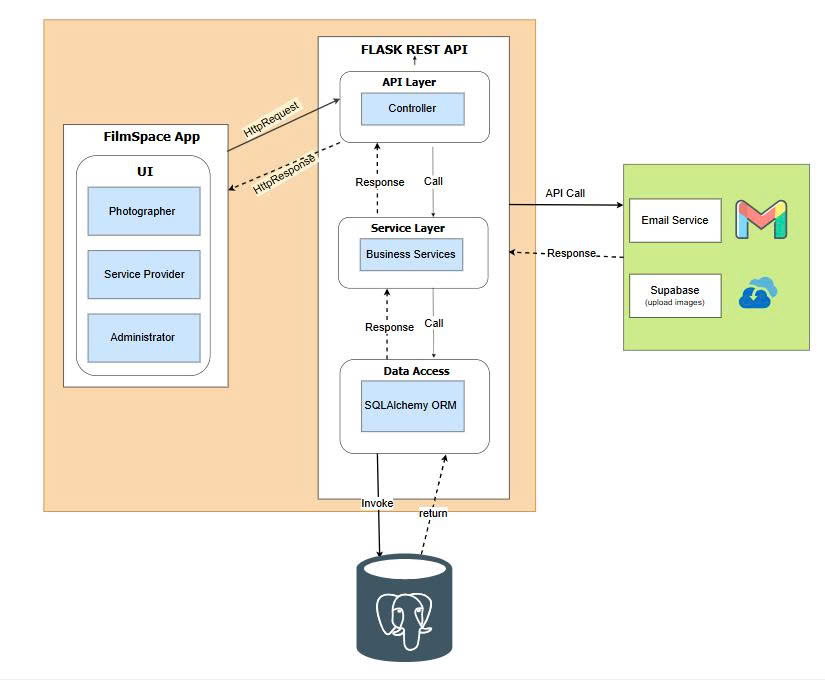
\includegraphics[width=\textwidth]{images/5.jpg}
	\caption{Kiến trúc tổng thể của hệ thống}
	\label{fig:system-arcFronthitecture}
\end{figure}

\subsubsection{Frontend}

Frontend của hệ thống được xây dựng dưới dạng ứng dụng Web, sử dụng
HTML, CSS và JavaScript để xây dựng giao diện và xử lý tương tác với người dùng.

\begin{itemize}
	\item \textbf{HTML:} Xây dựng cấu trúc các trang Web dành cho
	Photographer, Service Provider và Administrator.
	
	\item \textbf{CSS:} Thiết kế giao diện và bố cục cho các trang,
	bao gồm các thành phần dùng chung và giao diện theo từng nhóm người dùng.
	
	\item \textbf{JavaScript:} Xử lý tương tác, kiểm tra dữ liệu đầu vào
	và cập nhật nội dung động trên giao diện.
	
	\item \textbf{Fetch API:} Gửi request từ Frontend đến các REST API
	của Backend để thực hiện xác thực, quản lý hồ sơ, tìm kiếm,
	Booking, Workshop, thanh toán và các chức năng quản trị.
\end{itemize}

\begin{figure}[H]
	\centering
	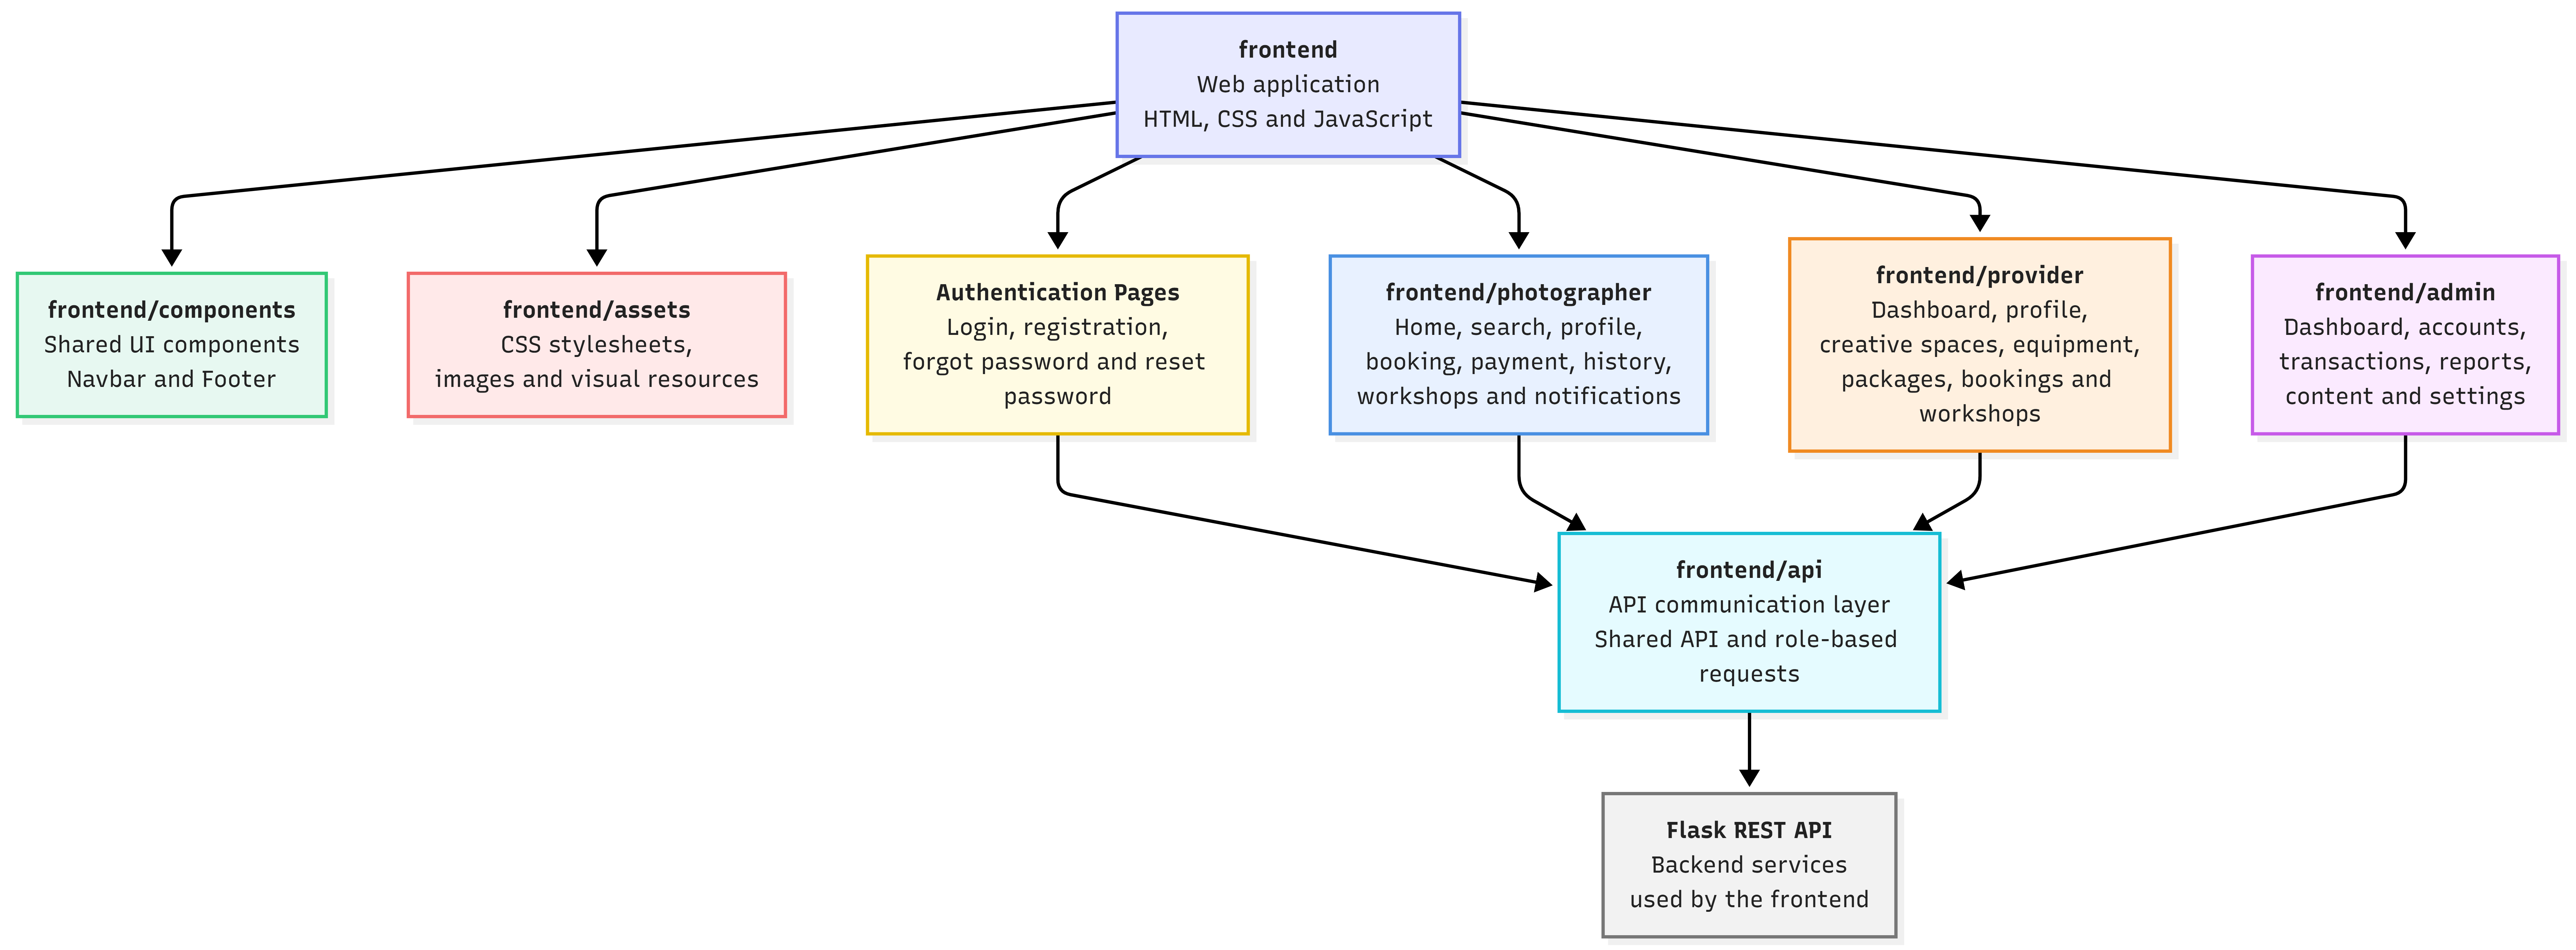
\includegraphics[width=\textwidth]{images/8.png}
	\caption{Kiến trúc Frontend}
	\label{fig:frontend-architecture}
\end{figure}


\subsubsection{Backend}

Backend của hệ thống được xây dựng bằng Flask theo kiến trúc
Clean Architecture, cung cấp các REST API và xử lý nghiệp vụ của hệ thống.

\begin{itemize}
	\item \textbf{Flask:} Framework chính để xây dựng Backend và cung cấp
	các REST API cho Frontend.
	
	\item \textbf{Clean Architecture:} Tổ chức Backend thành các lớp
	API, Services, Domain và Infrastructure, giúp phân tách trách nhiệm
	và hỗ trợ bảo trì hệ thống.
	
	
	\item \textbf{PostgreSQL:} Hệ quản trị cơ sở dữ liệu quan hệ,
	lưu trữ thông tin người dùng, Service Provider, Creative Space,
	Equipment, Booking, Workshop, Invoice, Payment và Notification.
	
	
	\item \textbf{Email Service:} Hỗ trợ gửi mã OTP phục vụ chức năng
	quên mật khẩu và đặt lại mật khẩu.
\end{itemize}

\begin{figure}[H]
	\centering
	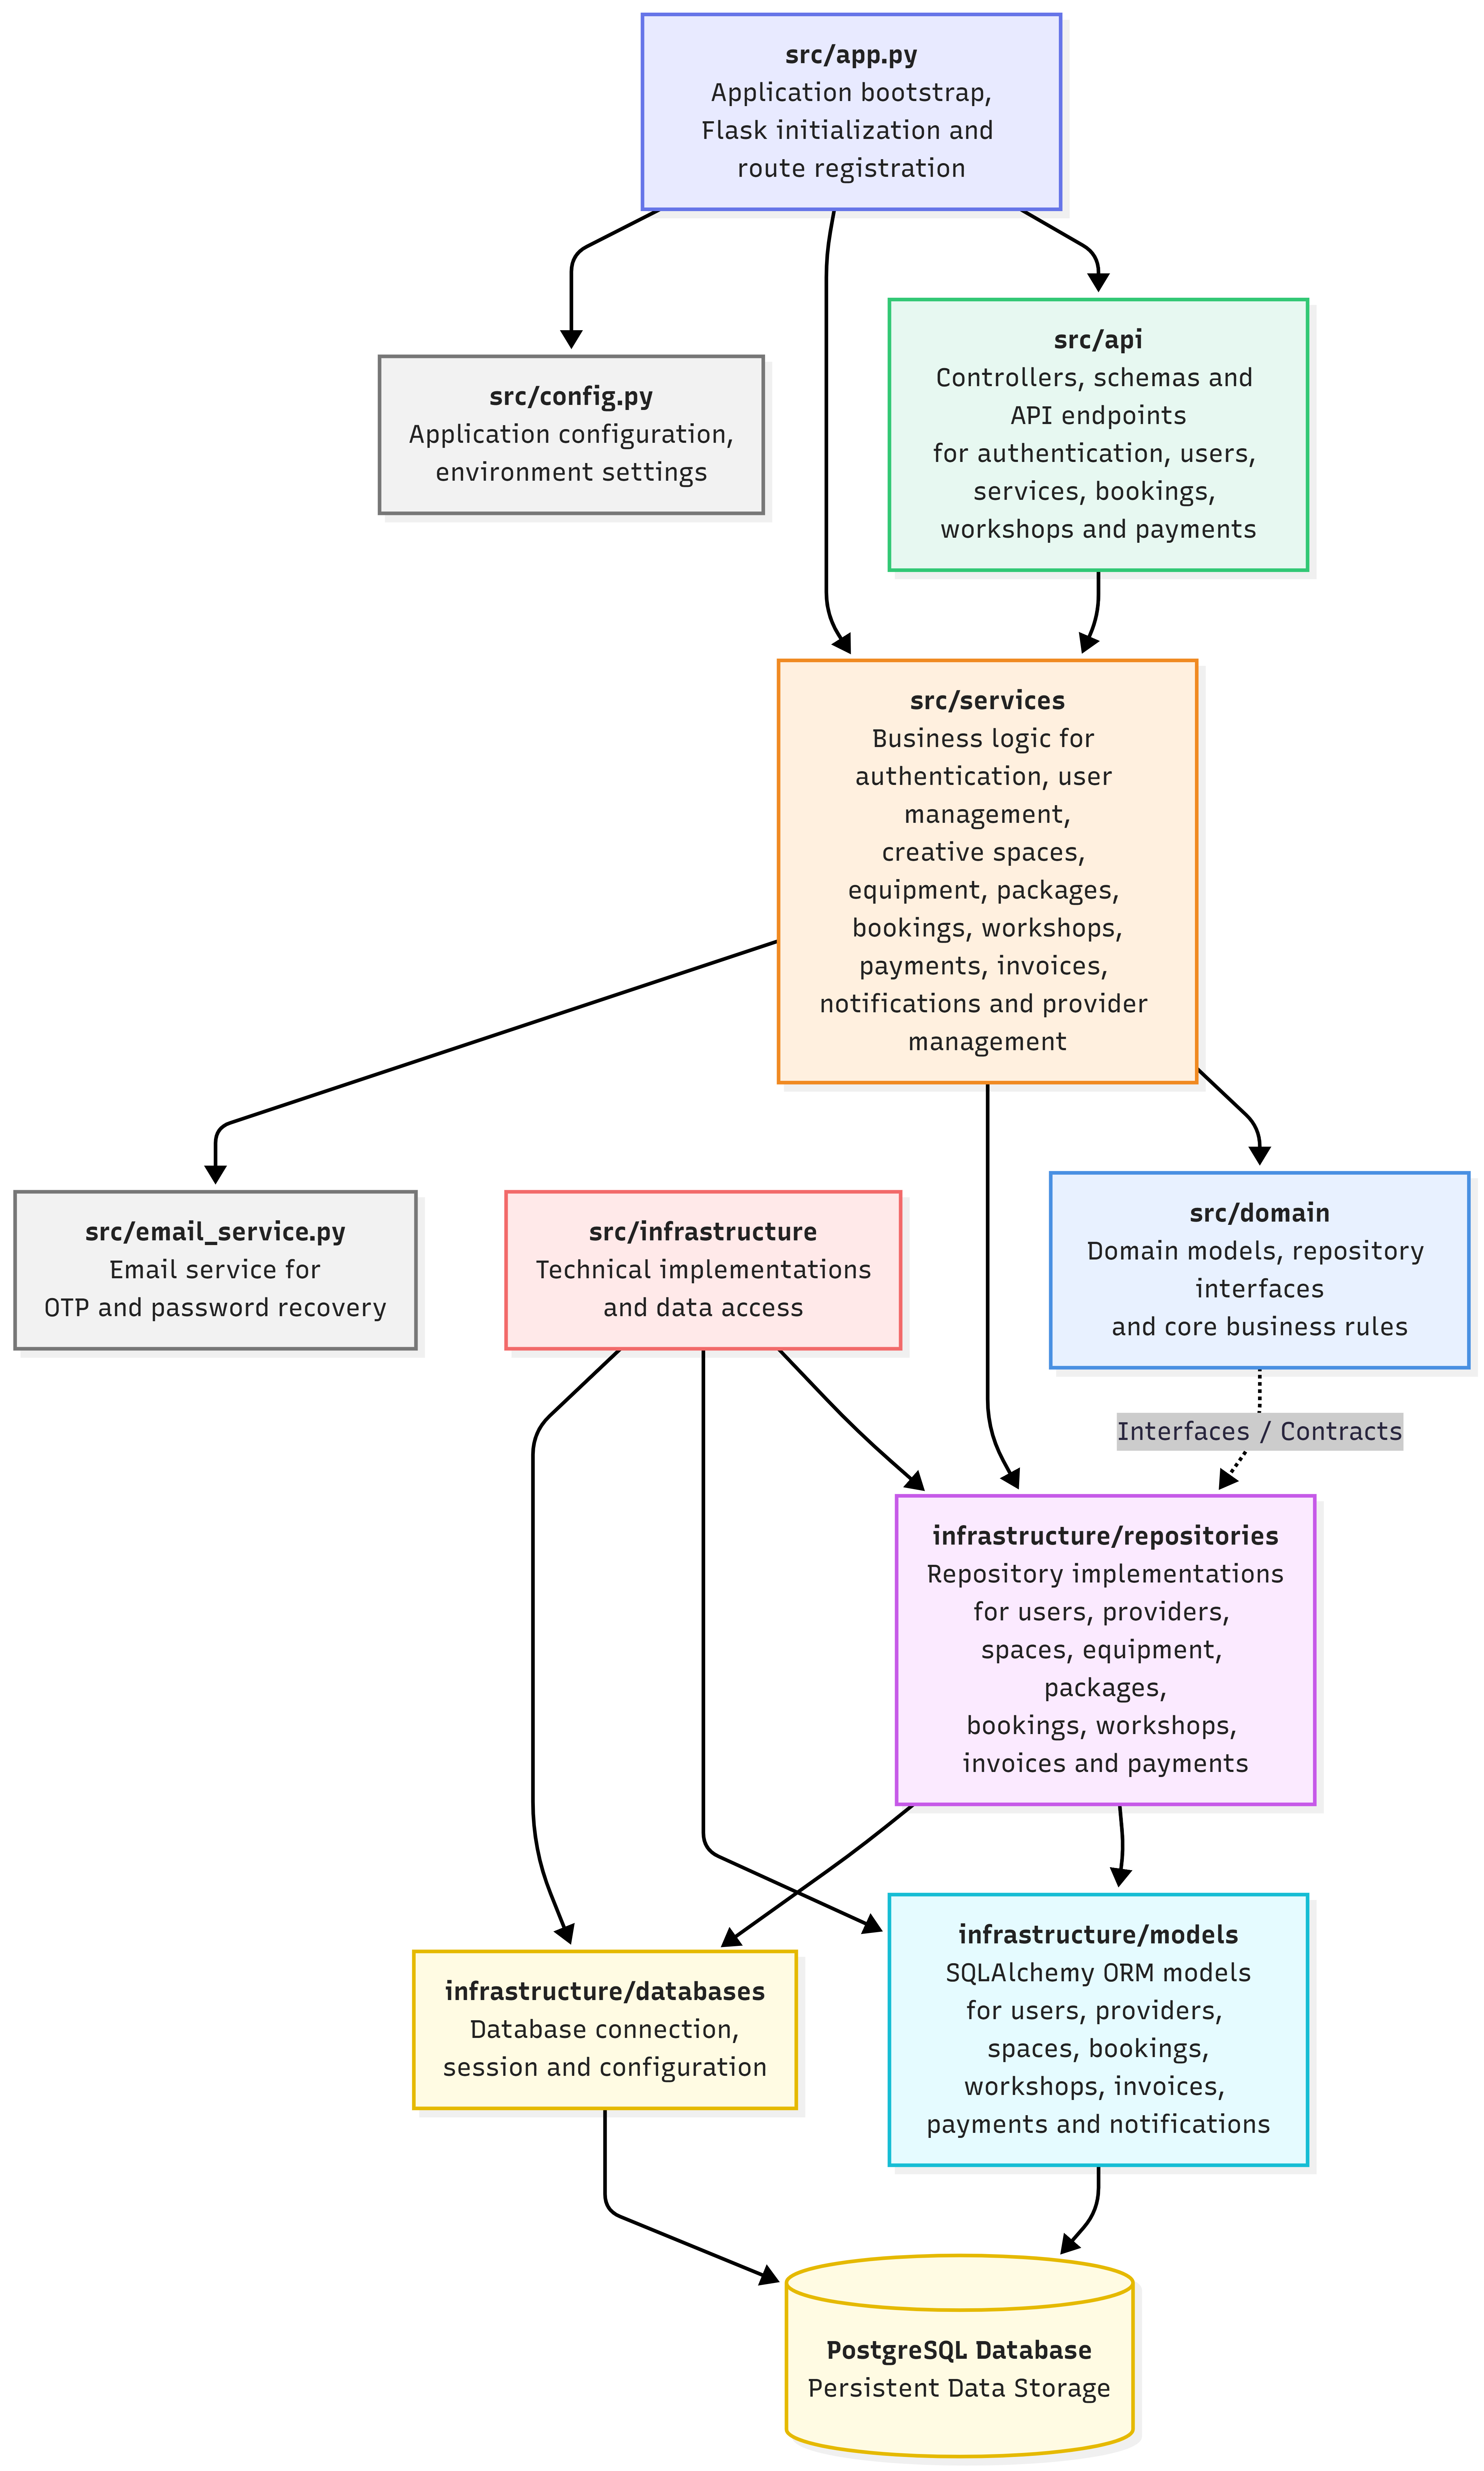
\includegraphics[width=\textwidth]{images/9.png}
	\caption{Kiến trúc Backend}
	\label{fig:backend-architecture}
\end{figure}

\subsubsection{Third-party}

\begin{itemize}
	\item \textbf{GitHub:} Nền tảng quản lý mã nguồn, được sử dụng để
	lưu trữ source code và hỗ trợ quản lý phiên bản trong quá trình
	phát triển hệ thống.
	
	\item \textbf{Supabase:} Nền tảng cung cấp dịch vụ PostgreSQL,
	được sử dụng để lưu trữ và quản lý dữ liệu của hệ thống.
\end{itemize}
\subsection{Package Diagram}
\subsubsection{Frontend}

\begin{figure}[H]
	\centering
	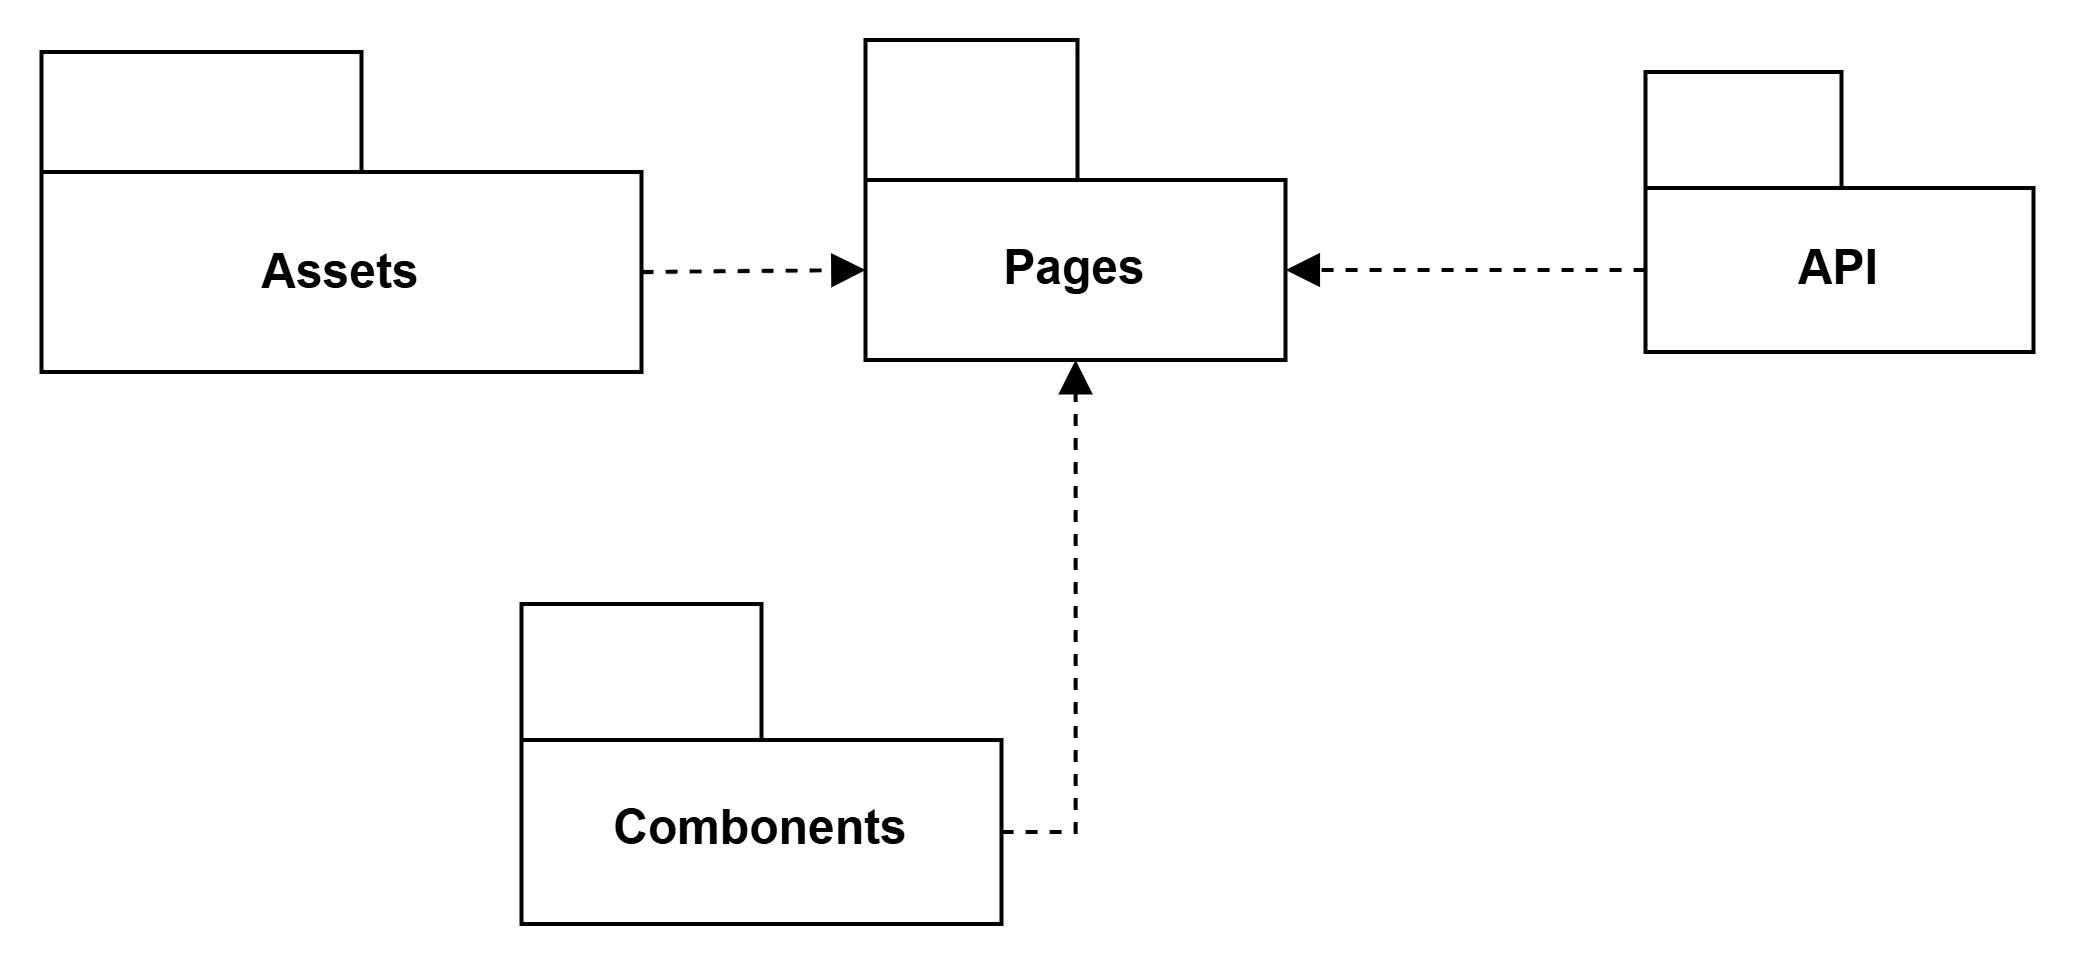
\includegraphics[width=\textwidth]{images/4.jpg}
	\caption{Package Diagram của Frontend}
	\label{fig:package-diagram-frontend}
\end{figure}

\begin{longtable}{
		|>{\raggedright\arraybackslash}p{0.8cm}|
		>{\raggedright\arraybackslash}p{4.0cm}|
		>{\raggedright\arraybackslash}p{8.0cm}|
	}
	\caption{Các package chính của Frontend}
	\label{tab:frontend-packages}\\
	\hline
	\textbf{No} & \textbf{Package} & \textbf{Description} \\ \hline
	\endfirsthead
	
	\hline
	\textbf{No} & \textbf{Package} & \textbf{Description} \\ \hline
	\endhead
	
	1 & frontend &
	Thư mục gốc chứa mã nguồn Frontend của ứng dụng Web. \\ \hline
	
	2 & authentication &
	Chứa các trang đăng nhập, đăng ký, xác thực OTP,
	quên mật khẩu và đặt lại mật khẩu. \\ \hline
	
	3 & photographer &
	Chứa các trang dành cho Photographer như trang chủ,
	tìm kiếm, hồ sơ, Booking, thanh toán, lịch sử,
	Workshop và thông báo. \\ \hline
	
	4 & provider &
	Chứa các trang dành cho Service Provider như Dashboard,
	hồ sơ, Creative Space, Equipment, Service Package,
	Booking và Workshop. \\ \hline
	
	5 & admin &
	Chứa các trang quản trị như Dashboard, quản lý người dùng,
	Provider, phê duyệt Provider và giao dịch. \\ \hline
	
	6 & components &
	Chứa các thành phần giao diện dùng chung như Navbar và Footer. \\ \hline
	
	7 & api &
	Chứa các module JavaScript hỗ trợ giao tiếp với REST API. \\ \hline
	
	8 & assets &
	Chứa các tài nguyên giao diện như CSS và hình ảnh. \\ \hline
	
\end{longtable}


\subsubsection{Backend}

\begin{figure}[H]
	\centering
	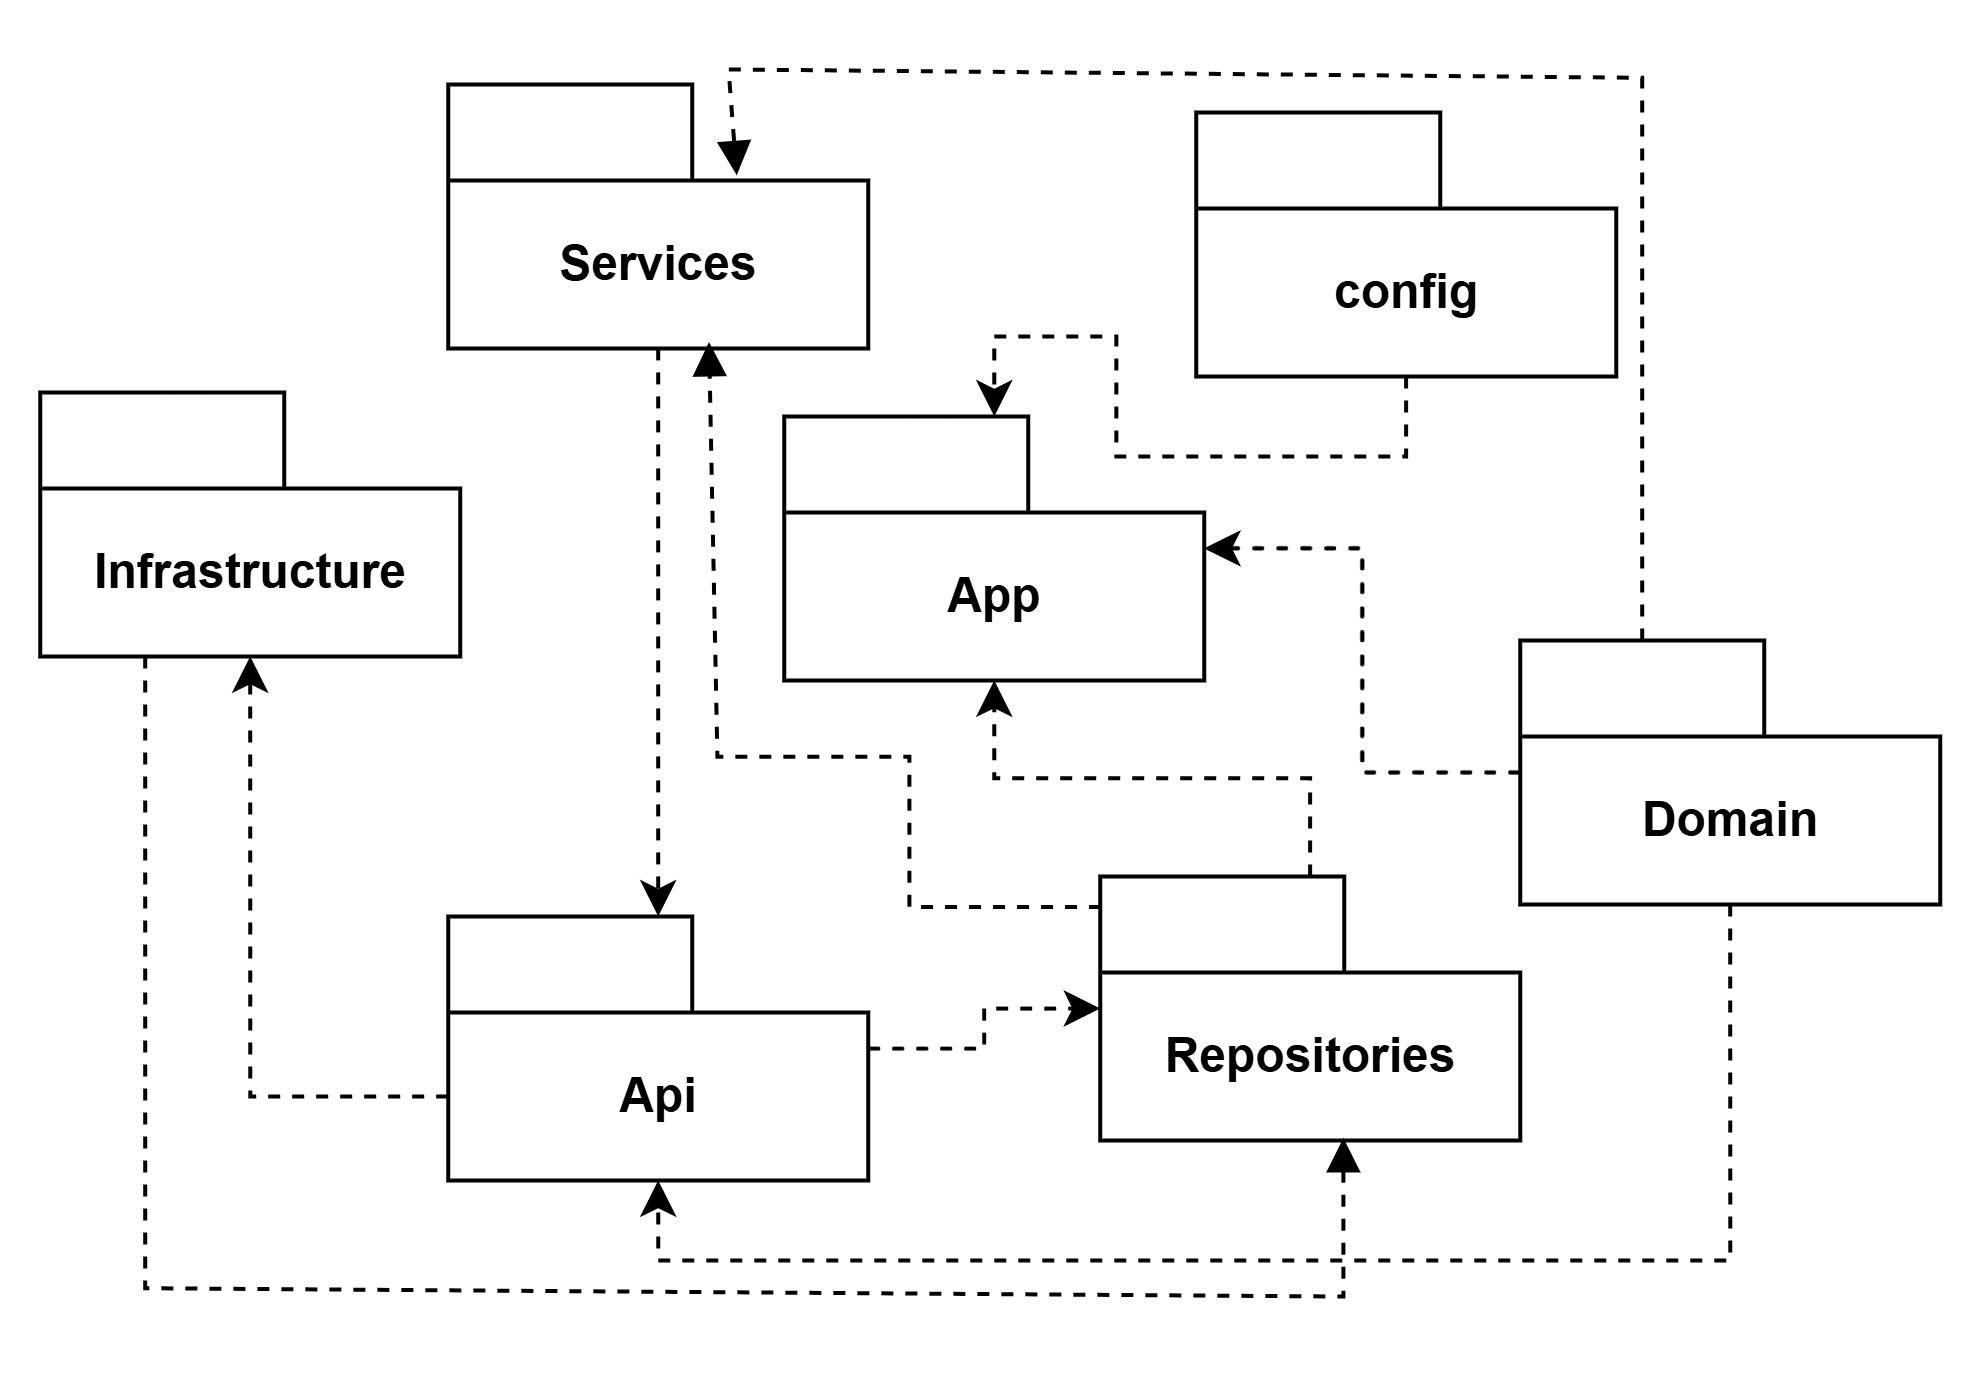
\includegraphics[width=\textwidth]{images/3.jpg}
	\caption{Package Diagram của Backend}
	\label{fig:package-diagram-backend}
\end{figure}

\begin{longtable}{
		|>{\raggedright\arraybackslash}p{0.8cm}|
		>{\raggedright\arraybackslash}p{4.0cm}|
		>{\raggedright\arraybackslash}p{8.0cm}|
	}
	\caption{Các package chính của Backend}
	\label{tab:backend-packages}\\
	\hline
	\textbf{No} & \textbf{Package} & \textbf{Description} \\ \hline
	\endfirsthead
	
	\hline
	\textbf{No} & \textbf{Package} & \textbf{Description} \\ \hline
	\endhead
	
	1 & src &
	Thư mục gốc chứa mã nguồn Backend của hệ thống. \\ \hline
	
	2 & src/api &
	Chứa Controllers, Schemas và các REST API endpoints. \\ \hline
	
	3 & src/services &
	Chứa xử lý nghiệp vụ cho Authentication, User, Creative Space,
	Equipment, Service Package, Booking, Workshop, Invoice,
	Payment, Notification và Provider. \\ \hline
	
	4 & src/domain &
	Chứa Domain Models, Repository Interfaces
	và các quy tắc nghiệp vụ cốt lõi. \\ \hline
	
	5 & src/infrastructure &
	Chứa các thành phần triển khai kỹ thuật
	và truy cập dữ liệu. \\ \hline
	
	6 & infrastructure /repositories &
	Chứa các Repository thực hiện truy xuất và thao tác dữ liệu. \\ \hline
	
	7 & infrastructure/models &
	Chứa các SQLAlchemy ORM Models và ánh xạ cơ sở dữ liệu. \\ \hline
	
	8 & infrastructure/databases &
	Chứa các thành phần quản lý kết nối và Database Session. \\ \hline
	
	9 & src/config.py &
	Chứa cấu hình ứng dụng và các thiết lập môi trường. \\ \hline
	
	10 & src/email\_service.py &
	Cung cấp dịch vụ Email cho OTP và khôi phục mật khẩu. \\ \hline
	
\end{longtable}

\section{Database Design}

Cơ sở dữ liệu của hệ thống được thiết kế theo mô hình quan hệ nhằm
đảm bảo tính nhất quán giữa tài khoản người dùng, Service Provider,
Creative Space, Equipment, Booking, Workshop, Invoice, Payment và
Notification. Các thực thể chính và mối quan hệ giữa chúng được thể hiện
trong sơ đồ Entity Relationship Diagram dưới đây.

\begin{figure}[H]
	\centering
	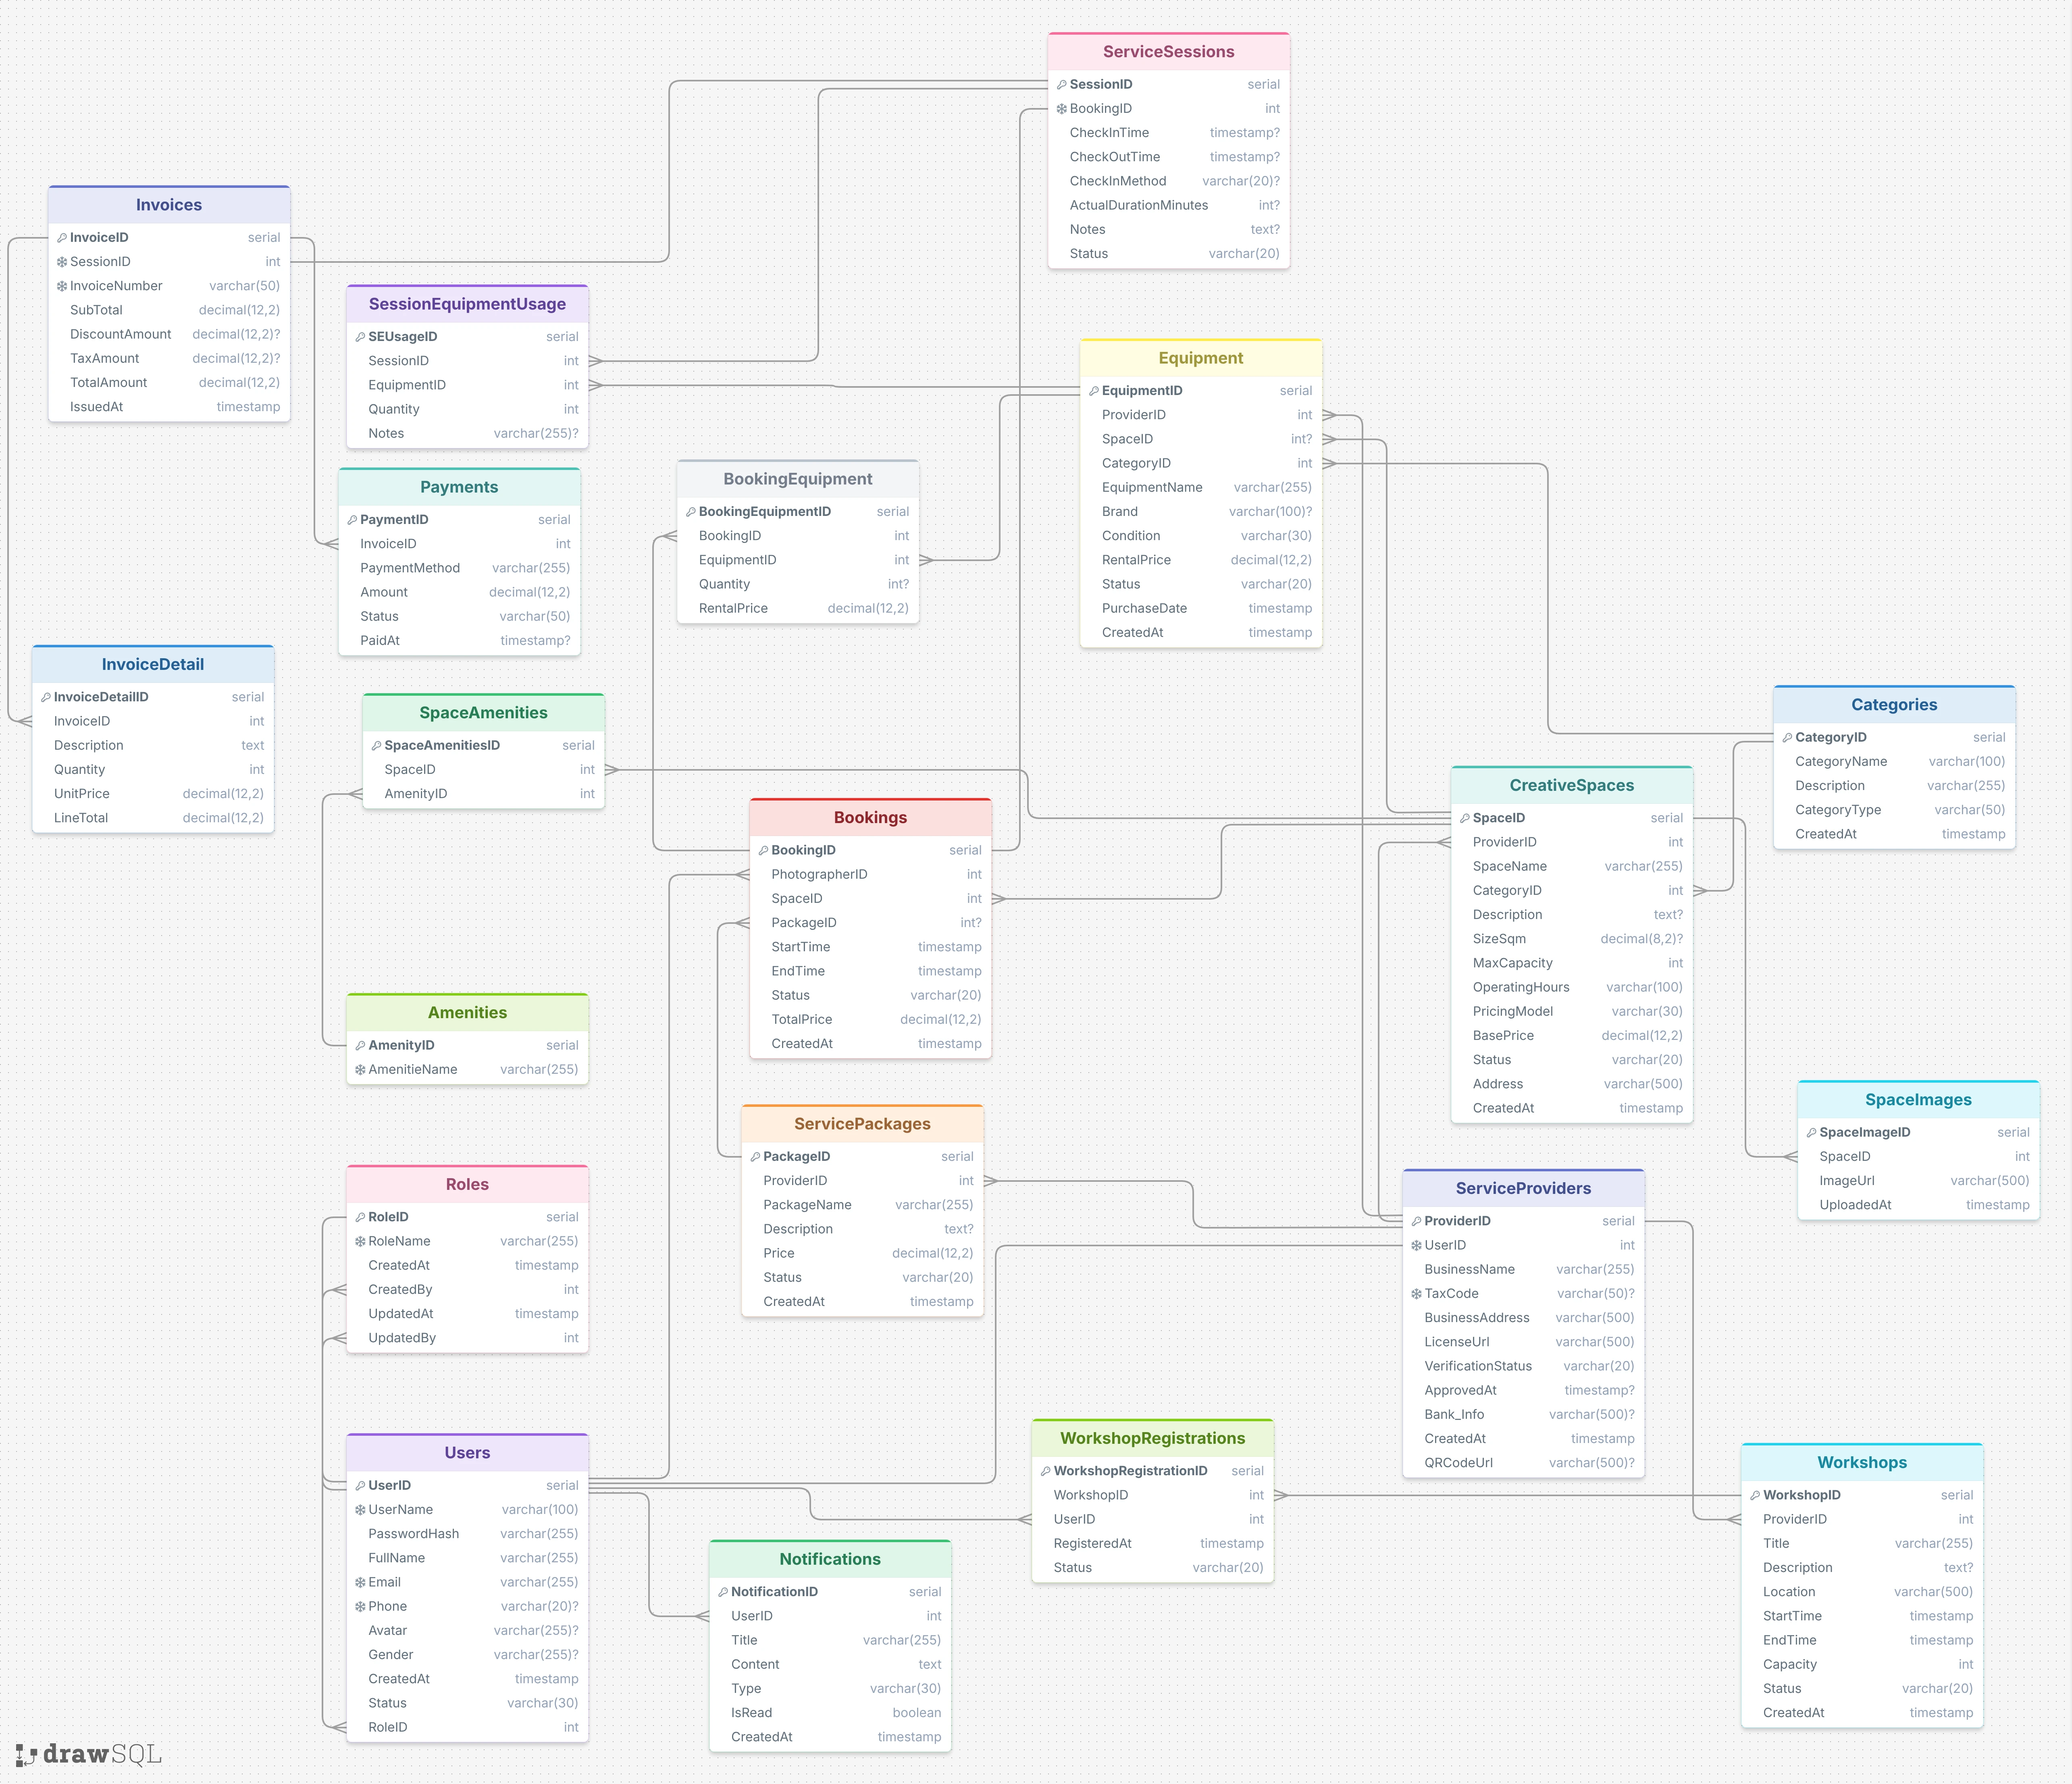
\includegraphics[width=\textwidth]{images/7.png}
	\caption{Entity Relationship Diagram}
	\label{fig:entity-relationship-diagram}
\end{figure}


\subsection{Database Tables Overview}

Cơ sở dữ liệu của hệ thống gồm 20 bảng chính. Các bảng hỗ trợ quản lý
tài khoản và phân quyền, Service Provider, Creative Space, Equipment,
Booking, Service Package, Service Session, Workshop, Invoice, Payment
và Notification.

\subsection{Users Table}

\begin{longtable}{
		|>{\raggedright\arraybackslash}p{3.2cm}|
		>{\raggedright\arraybackslash}p{4.2cm}|
		>{\raggedright\arraybackslash}p{5.0cm}|
	}
	\caption{Users Table Description}
	\label{tab:users}\\
	\hline
	\textbf{Field} & \textbf{Type} & \textbf{Description} \\ \hline
	\endfirsthead
	\hline
	\textbf{Field} & \textbf{Type} & \textbf{Description} \\ \hline
	\endhead
	
	UserID & INT, PK, IDENTITY &
	Unique identifier of the user account. \\ \hline
	
	UserName & VARCHAR(100), UNIQUE, NOT NULL &
	Username used to identify the account. \\ \hline
	
	PasswordHash & VARCHAR(255), NOT NULL &
	Hashed password of the user. \\ \hline
	
	FullName & VARCHAR(255), NOT NULL &
	Full name of the user. \\ \hline
	
	Email & VARCHAR(255), UNIQUE, NOT NULL &
	Email address of the user. \\ \hline
	
	Phone & VARCHAR(20), UNIQUE, NULL &
	Phone number of the user. \\ \hline
	
	Avatar & VARCHAR(255), NULL &
	Path or URL of the user's avatar. \\ \hline
	
	Gender & VARCHAR(255), NULL &
	Gender information of the user. \\ \hline
	
	CreatedAt & DATETIME, NOT NULL &
	Account creation time. \\ \hline
	
	Status & VARCHAR(30), NOT NULL &
	Current status of the user account. \\ \hline
	
	RoleID & INT, FK, NOT NULL &
	Reference to the user's role. \\ \hline
	
\end{longtable}


\subsection{Roles Table}

\begin{longtable}{
		|>{\raggedright\arraybackslash}p{3.2cm}|
		>{\raggedright\arraybackslash}p{4.2cm}|
		>{\raggedright\arraybackslash}p{5.0cm}|
	}
	\caption{Roles Table Description}
	\label{tab:roles}\\
	\hline
	\textbf{Field} & \textbf{Type} & \textbf{Description} \\ \hline
	\endfirsthead
	\hline
	\textbf{Field} & \textbf{Type} & \textbf{Description} \\ \hline
	\endhead
	
	RoleID & INT, PK, IDENTITY &
	Unique identifier of the role. \\ \hline
	
	RoleName & VARCHAR(255), UNIQUE, NOT NULL &
	Name of the user role. \\ \hline
	
	CreatedAt & DATETIME, NOT NULL &
	Role creation time. \\ \hline
	
	CreatedBy & INT, FK, NOT NULL &
	User who created the role. \\ \hline
	
	UpdatedAt & DATETIME, NOT NULL &
	Time when the role was last updated. \\ \hline
	
	UpdatedBy & INT, FK, NOT NULL &
	User who last updated the role. \\ \hline
	
\end{longtable}


\subsection{ServiceProviders Table}

\begin{longtable}{
		|>{\raggedright\arraybackslash}p{3.2cm}|
		>{\raggedright\arraybackslash}p{4.2cm}|
		>{\raggedright\arraybackslash}p{5.0cm}|
	}
	\caption{ServiceProviders Table Description}
	\label{tab:service-providers}\\
	\hline
	\textbf{Field} & \textbf{Type} & \textbf{Description} \\ \hline
	\endfirsthead
	\hline
	\textbf{Field} & \textbf{Type} & \textbf{Description} \\ \hline
	\endhead
	
	ProviderID & INT, PK, IDENTITY &
	Unique identifier of the Service Provider. \\ \hline
	
	UserID & INT, FK, UNIQUE, NOT NULL &
	Reference to the corresponding user account. \\ \hline
	
	BusinessName & VARCHAR(255), NOT NULL &
	Business name of the Service Provider. \\ \hline
	
	TaxCode & VARCHAR(50), UNIQUE, NULL &
	Tax identification code of the Service Provider. \\ \hline
	
	BusinessAddress & VARCHAR(500), NOT NULL &
	Business address of the Service Provider. \\ \hline
	
	LicenseUrl & VARCHAR(500), NOT NULL &
	URL of the business license document. \\ \hline
	
	VerificationStatus & VARCHAR(20), NOT NULL &
	Verification status of the Service Provider. \\ \hline
	
	ApprovedAt & DATETIME, NULL &
	Time when the Service Provider was approved. \\ \hline
	
	Bank\_Info & VARCHAR(500), NULL &
	Banking information of the Service Provider. \\ \hline
	
	CreatedAt & DATETIME, NOT NULL &
	Provider record creation time. \\ \hline
	
	QRCodeUrl & VARCHAR(500), NULL &
	URL of the payment QR code. \\ \hline
	
\end{longtable}


\subsection{Categories Table}

\begin{longtable}{
		|>{\raggedright\arraybackslash}p{3.2cm}|
		>{\raggedright\arraybackslash}p{4.2cm}|
		>{\raggedright\arraybackslash}p{5.0cm}|
	}
	\caption{Categories Table Description}
	\label{tab:categories}\\
	\hline
	\textbf{Field} & \textbf{Type} & \textbf{Description} \\ \hline
	\endfirsthead
	\hline
	\textbf{Field} & \textbf{Type} & \textbf{Description} \\ \hline
	\endhead
	
	CategoryID & INT, PK, IDENTITY &
	Unique identifier of the category. \\ \hline
	
	CategoryName & VARCHAR(100), NOT NULL &
	Name of the category. \\ \hline
	
	Description & VARCHAR(255), NOT NULL &
	Description of the category. \\ \hline
	
	CategoryType & VARCHAR(50), NOT NULL &
	Type of the category. \\ \hline
	
	CreatedAt & DATETIME, NOT NULL &
	Category creation time. \\ \hline
	
\end{longtable}


\subsection{CreativeSpaces Table}

\begin{longtable}{
		|>{\raggedright\arraybackslash}p{3.2cm}|
		>{\raggedright\arraybackslash}p{4.2cm}|
		>{\raggedright\arraybackslash}p{5.0cm}|
	}
	\caption{CreativeSpaces Table Description}
	\label{tab:creative-spaces}\\
	\hline
	\textbf{Field} & \textbf{Type} & \textbf{Description} \\ \hline
	\endfirsthead
	\hline
	\textbf{Field} & \textbf{Type} & \textbf{Description} \\ \hline
	\endhead
	
	SpaceID & INT, PK, IDENTITY &
	Unique identifier of the Creative Space. \\ \hline
	
	ProviderID & INT, FK, NOT NULL &
	Reference to the Service Provider. \\ \hline
	
	SpaceName & VARCHAR(255), NOT NULL &
	Name of the Creative Space. \\ \hline
	
	CategoryID & INT, FK, NOT NULL &
	Reference to the space category. \\ \hline
	
	Description & TEXT, NULL &
	Detailed description of the Creative Space. \\ \hline
	
	SizeSqm & NUMERIC(8,2), NULL &
	Area of the Creative Space in square meters. \\ \hline
	
	MaxCapacity & INT, NOT NULL &
	Maximum capacity of the Creative Space. \\ \hline
	
	OperatingHours & VARCHAR(100), NOT NULL &
	Operating hours of the Creative Space. \\ \hline
	
	PricingModel & VARCHAR(30), NOT NULL &
	Pricing model of the Creative Space. \\ \hline
	
	BasePrice & NUMERIC(12,2), NOT NULL &
	Base price of the Creative Space. \\ \hline
	
	Status & VARCHAR(20), NOT NULL &
	Current status of the Creative Space. \\ \hline
	
	Address & VARCHAR(500), NOT NULL &
	Address of the Creative Space. \\ \hline
	
	CreatedAt & DATETIME, NOT NULL &
	Space creation time. \\ \hline
	
\end{longtable}


\subsection{SpaceImages Table}

\begin{longtable}{
		|>{\raggedright\arraybackslash}p{3.2cm}|
		>{\raggedright\arraybackslash}p{4.2cm}|
		>{\raggedright\arraybackslash}p{5.0cm}|
	}
	\caption{SpaceImages Table Description}
	\label{tab:space-images}\\
	\hline
	\textbf{Field} & \textbf{Type} & \textbf{Description} \\ \hline
	\endfirsthead
	\hline
	\textbf{Field} & \textbf{Type} & \textbf{Description} \\ \hline
	\endhead
	
	SpaceImageID & INT, PK, IDENTITY &
	Unique identifier of the space image. \\ \hline
	
	SpaceID & INT, FK, NOT NULL &
	Reference to the Creative Space. \\ \hline
	
	ImageUrl & VARCHAR(500), NOT NULL &
	URL of the Creative Space image. \\ \hline
	
	UploadedAt & DATETIME, NOT NULL &
	Image upload time. \\ \hline
	
\end{longtable}


\subsection{Amenities Table}

\begin{longtable}{
		|>{\raggedright\arraybackslash}p{3.2cm}|
		>{\raggedright\arraybackslash}p{4.2cm}|
		>{\raggedright\arraybackslash}p{5.0cm}|
	}
	\caption{Amenities Table Description}
	\label{tab:amenities}\\
	\hline
	\textbf{Field} & \textbf{Type} & \textbf{Description} \\ \hline
	\endfirsthead
	\hline
	\textbf{Field} & \textbf{Type} & \textbf{Description} \\ \hline
	\endhead
	
	AmenityID & INT, PK, IDENTITY &
	Unique identifier of the amenity. \\ \hline
	
	AmenitieName & VARCHAR(255), UNIQUE, NOT NULL &
	Name of the amenity. \\ \hline
	
\end{longtable}


\subsection{SpaceAmenities Table}

\begin{longtable}{
		|>{\raggedright\arraybackslash}p{3.2cm}|
		>{\raggedright\arraybackslash}p{4.2cm}|
		>{\raggedright\arraybackslash}p{5.0cm}|
	}
	\caption{SpaceAmenities Table Description}
	\label{tab:space-amenities}\\
	\hline
	\textbf{Field} & \textbf{Type} & \textbf{Description} \\ \hline
	\endfirsthead
	\hline
	\textbf{Field} & \textbf{Type} & \textbf{Description} \\ \hline
	\endhead
	
	SpaceAmenitiesID & INT, PK, IDENTITY &
	Unique identifier of the space-amenity record. \\ \hline
	
	SpaceID & INT, FK, NOT NULL &
	Reference to the Creative Space. \\ \hline
	
	AmenityID & INT, FK, NOT NULL &
	Reference to the amenity. \\ \hline
	
\end{longtable}


\subsection{Equipment Table}

\begin{longtable}{
		|>{\raggedright\arraybackslash}p{3.2cm}|
		>{\raggedright\arraybackslash}p{4.2cm}|
		>{\raggedright\arraybackslash}p{5.0cm}|
	}
	\caption{Equipment Table Description}
	\label{tab:equipment}\\
	\hline
	\textbf{Field} & \textbf{Type} & \textbf{Description} \\ \hline
	\endfirsthead
	\hline
	\textbf{Field} & \textbf{Type} & \textbf{Description} \\ \hline
	\endhead
	
	EquipmentID & INT, PK, IDENTITY &
	Unique identifier of the equipment. \\ \hline
	
	ProviderID & INT, FK, NOT NULL &
	Reference to the Service Provider. \\ \hline
	
	SpaceID & INT, FK, NULL &
	Reference to the Creative Space associated with the equipment. \\ \hline
	
	CategoryID & INT, FK, NOT NULL &
	Reference to the equipment category. \\ \hline
	
	EquipmentName & VARCHAR(255), NOT NULL &
	Name of the equipment. \\ \hline
	
	Brand & VARCHAR(100), NULL &
	Brand of the equipment. \\ \hline
	
	Condition & VARCHAR(30), NOT NULL &
	Current physical condition of the equipment. \\ \hline
	
	RentalPrice & NUMERIC(12,2), NOT NULL &
	Rental price of the equipment. \\ \hline
	
	Status & VARCHAR(20), NOT NULL &
	Current status of the equipment. \\ \hline
	
	PurchaseDate & DATETIME, NOT NULL &
	Purchase date of the equipment. \\ \hline
	
	CreatedAt & DATETIME, NOT NULL &
	Equipment creation time. \\ \hline
	
\end{longtable}


\subsection{Bookings Table}

\begin{longtable}{
		|>{\raggedright\arraybackslash}p{3.2cm}|
		>{\raggedright\arraybackslash}p{4.2cm}|
		>{\raggedright\arraybackslash}p{5.0cm}|
	}
	\caption{Bookings Table Description}
	\label{tab:bookings}\\
	\hline
	\textbf{Field} & \textbf{Type} & \textbf{Description} \\ \hline
	\endfirsthead
	\hline
	\textbf{Field} & \textbf{Type} & \textbf{Description} \\ \hline
	\endhead
	
	BookingID & INT, PK, IDENTITY &
	Unique identifier of the Booking. \\ \hline
	
	PhotographerID & INT, FK, NOT NULL &
	Reference to the Photographer user. \\ \hline
	
	SpaceID & INT, FK, NOT NULL &
	Reference to the booked Creative Space. \\ \hline
	
	PackageID & INT, FK, NULL &
	Reference to the selected Service Package. \\ \hline
	
	StartTime & DATETIME, NOT NULL &
	Booking start time. \\ \hline
	
	EndTime & DATETIME, NOT NULL &
	Booking end time. \\ \hline
	
	Status & VARCHAR(20), NOT NULL &
	Current status of the Booking. \\ \hline
	
	TotalPrice & NUMERIC(12,2), NOT NULL &
	Total price of the Booking. \\ \hline
	
	CreatedAt & DATETIME, NOT NULL &
	Booking creation time. \\ \hline
	
\end{longtable}


\subsection{BookingEquipment Table}

\begin{longtable}{
		|>{\raggedright\arraybackslash}p{3.2cm}|
		>{\raggedright\arraybackslash}p{4.2cm}|
		>{\raggedright\arraybackslash}p{5.0cm}|
	}
	\caption{BookingEquipment Table Description}
	\label{tab:booking-equipment}\\
	\hline
	\textbf{Field} & \textbf{Type} & \textbf{Description} \\ \hline
	\endfirsthead
	\hline
	\textbf{Field} & \textbf{Type} & \textbf{Description} \\ \hline
	\endhead
	
	BookingEquipmentID & INT, PK, IDENTITY &
	Unique identifier of the Booking equipment record. \\ \hline
	
	BookingID & INT, FK, NOT NULL &
	Reference to the Booking. \\ \hline
	
	EquipmentID & INT, FK, NOT NULL &
	Reference to the selected equipment. \\ \hline
	
	Quantity & INT, NULL &
	Quantity of the selected equipment. \\ \hline
	
	RentalPrice & NUMERIC(12,2), NOT NULL &
	Rental price of the equipment. \\ \hline
	
\end{longtable}


\subsection{ServiceSessions Table}

\begin{longtable}{
		|>{\raggedright\arraybackslash}p{3.2cm}|
		>{\raggedright\arraybackslash}p{4.2cm}|
		>{\raggedright\arraybackslash}p{5.0cm}|
	}
	\caption{ServiceSessions Table Description}
	\label{tab:service-sessions}\\
	\hline
	\textbf{Field} & \textbf{Type} & \textbf{Description} \\ \hline
	\endfirsthead
	\hline
	\textbf{Field} & \textbf{Type} & \textbf{Description} \\ \hline
	\endhead
	
	SessionID & INT, PK, IDENTITY &
	Unique identifier of the service session. \\ \hline
	
	BookingID & INT, FK, UNIQUE, NOT NULL &
	Reference to the Booking. \\ \hline
	
	CheckInTime & DATETIME, NULL &
	Check-in time of the Photographer. \\ \hline
	
	CheckOutTime & DATETIME, NULL &
	Check-out time of the Photographer. \\ \hline
	
	CheckInMethod & VARCHAR(20), NULL &
	Method used for check-in. \\ \hline
	
	ActualDurationMinutes & INT, NULL &
	Actual service duration in minutes. \\ \hline
	
	Notes & TEXT, NULL &
	Additional notes about the service session. \\ \hline
	
	Status & VARCHAR(20), NOT NULL &
	Current status of the service session. \\ \hline
	
\end{longtable}


\subsection{SessionEquipmentUsage Table}

\begin{longtable}{
		|>{\raggedright\arraybackslash}p{3.2cm}|
		>{\raggedright\arraybackslash}p{4.2cm}|
		>{\raggedright\arraybackslash}p{5.0cm}|
	}
	\caption{SessionEquipmentUsage Table Description}
	\label{tab:session-equipment-usage}\\
	\hline
	\textbf{Field} & \textbf{Type} & \textbf{Description} \\ \hline
	\endfirsthead
	\hline
	\textbf{Field} & \textbf{Type} & \textbf{Description} \\ \hline
	\endhead
	
	SEUsageID & INT, PK, IDENTITY &
	Unique identifier of the equipment usage record. \\ \hline
	
	SessionID & INT, FK, NOT NULL &
	Reference to the service session. \\ \hline
	
	EquipmentID & INT, FK, NOT NULL &
	Reference to the used equipment. \\ \hline
	
	Quantity & INT, NOT NULL &
	Quantity of equipment used. \\ \hline
	
	Notes & VARCHAR(255), NULL &
	Additional notes about equipment usage. \\ \hline
	
\end{longtable}


\subsection{ServicePackages Table}

\begin{longtable}{
		|>{\raggedright\arraybackslash}p{3.2cm}|
		>{\raggedright\arraybackslash}p{4.2cm}|
		>{\raggedright\arraybackslash}p{5.0cm}|
	}
	\caption{ServicePackages Table Description}
	\label{tab:service-packages}\\
	\hline
	\textbf{Field} & \textbf{Type} & \textbf{Description} \\ \hline
	\endfirsthead
	\hline
	\textbf{Field} & \textbf{Type} & \textbf{Description} \\ \hline
	\endhead
	
	PackageID & INT, PK, IDENTITY &
	Unique identifier of the Service Package. \\ \hline
	
	ProviderID & INT, FK, NOT NULL &
	Reference to the Service Provider. \\ \hline
	
	PackageName & VARCHAR(255), NOT NULL &
	Name of the Service Package. \\ \hline
	
	Description & TEXT, NULL &
	Description of the Service Package. \\ \hline
	
	Price & NUMERIC(12,2), NOT NULL &
	Price of the Service Package. \\ \hline
	
	Status & VARCHAR(20), NOT NULL &
	Current status of the Service Package. \\ \hline
	
	CreatedAt & DATETIME, NOT NULL &
	Package creation time. \\ \hline
	
\end{longtable}


\subsection{Invoices Table}

\begin{longtable}{
		|>{\raggedright\arraybackslash}p{3.2cm}|
		>{\raggedright\arraybackslash}p{4.2cm}|
		>{\raggedright\arraybackslash}p{5.0cm}|
	}
	\caption{Invoices Table Description}
	\label{tab:invoices}\\
	\hline
	\textbf{Field} & \textbf{Type} & \textbf{Description} \\ \hline
	\endfirsthead
	\hline
	\textbf{Field} & \textbf{Type} & \textbf{Description} \\ \hline
	\endhead
	
	InvoiceID & INT, PK, IDENTITY &
	Unique identifier of the invoice. \\ \hline
	
	SessionID & INT, FK, UNIQUE, NOT NULL &
	Reference to the service session. \\ \hline
	
	InvoiceNumber & VARCHAR(50), UNIQUE, NOT NULL &
	Unique invoice number. \\ \hline
	
	SubTotal & NUMERIC(12,2), NOT NULL &
	Subtotal amount before discount and tax. \\ \hline
	
	DiscountAmount & NUMERIC(12,2), NULL &
	Discount amount applied to the invoice. \\ \hline
	
	TaxAmount & NUMERIC(12,2), NULL &
	Tax amount applied to the invoice. \\ \hline
	
	TotalAmount & NUMERIC(12,2), NOT NULL &
	Final total amount of the invoice. \\ \hline
	
	IssuedAt & DATETIME, NOT NULL &
	Invoice issue time. \\ \hline
	
\end{longtable}


\subsection{InvoiceDetail Table}

\begin{longtable}{
		|>{\raggedright\arraybackslash}p{3.2cm}|
		>{\raggedright\arraybackslash}p{4.2cm}|
		>{\raggedright\arraybackslash}p{5.0cm}|
	}
	\caption{InvoiceDetail Table Description}
	\label{tab:invoice-detail}\\
	\hline
	\textbf{Field} & \textbf{Type} & \textbf{Description} \\ \hline
	\endfirsthead
	\hline
	\textbf{Field} & \textbf{Type} & \textbf{Description} \\ \hline
	\endhead
	
	InvoiceDetailID & INT, PK, IDENTITY &
	Unique identifier of the invoice detail. \\ \hline
	
	InvoiceID & INT, FK, NOT NULL &
	Reference to the invoice. \\ \hline
	
	Description & TEXT, NOT NULL &
	Description of the invoice item. \\ \hline
	
	Quantity & INT, NOT NULL &
	Quantity of the invoice item. \\ \hline
	
	UnitPrice & NUMERIC(12,2), NOT NULL &
	Unit price of the invoice item. \\ \hline
	
	LineTotal & NUMERIC(12,2), NOT NULL &
	Total amount of the invoice item. \\ \hline
	
\end{longtable}


\subsection{Payments Table}

\begin{longtable}{
		|>{\raggedright\arraybackslash}p{3.2cm}|
		>{\raggedright\arraybackslash}p{4.2cm}|
		>{\raggedright\arraybackslash}p{5.0cm}|
	}
	\caption{Payments Table Description}
	\label{tab:payments}\\
	\hline
	\textbf{Field} & \textbf{Type} & \textbf{Description} \\ \hline
	\endfirsthead
	\hline
	\textbf{Field} & \textbf{Type} & \textbf{Description} \\ \hline
	\endhead
	
	PaymentID & INT, PK, IDENTITY &
	Unique identifier of the payment. \\ \hline
	
	InvoiceID & INT, FK, NOT NULL &
	Reference to the invoice being paid. \\ \hline
	
	PaymentMethod & VARCHAR(255), NOT NULL &
	Payment method used by the Photographer. \\ \hline
	
	Amount & NUMERIC(12,2), NOT NULL &
	Payment amount. \\ \hline
	
	Status & VARCHAR(50), NOT NULL &
	Current status of the payment. \\ \hline
	
	PaidAt & DATETIME, NULL &
	Time when the payment was completed. \\ \hline
	
\end{longtable}


\subsection{Workshops Table}

\begin{longtable}{
		|>{\raggedright\arraybackslash}p{3.2cm}|
		>{\raggedright\arraybackslash}p{4.2cm}|
		>{\raggedright\arraybackslash}p{5.0cm}|
	}
	\caption{Workshops Table Description}
	\label{tab:workshops}\\
	\hline
	\textbf{Field} & \textbf{Type} & \textbf{Description} \\ \hline
	\endfirsthead
	\hline
	\textbf{Field} & \textbf{Type} & \textbf{Description} \\ \hline
	\endhead
	
	WorkshopID & INT, PK, IDENTITY &
	Unique identifier of the Workshop. \\ \hline
	
	ProviderID & INT, FK, NOT NULL &
	Reference to the Service Provider. \\ \hline
	
	Title & VARCHAR(255), NOT NULL &
	Workshop title. \\ \hline
	
	Description & TEXT, NULL &
	Detailed Workshop description. \\ \hline
	
	Location & VARCHAR(500), NOT NULL &
	Workshop location. \\ \hline
	
	StartTime & DATETIME, NOT NULL &
	Workshop start time. \\ \hline
	
	EndTime & DATETIME, NOT NULL &
	Workshop end time. \\ \hline
	
	Capacity & INT, NOT NULL &
	Maximum number of participants. \\ \hline
	
	Status & VARCHAR(20), NOT NULL &
	Current status of the Workshop. \\ \hline
	
	CreatedAt & DATETIME, NOT NULL &
	Workshop creation time. \\ \hline
	
\end{longtable}


\subsection{WorkshopRegistrations Table}

\begin{longtable}{
		|>{\raggedright\arraybackslash}p{3.2cm}|
		>{\raggedright\arraybackslash}p{4.2cm}|
		>{\raggedright\arraybackslash}p{5.0cm}|
	}
	\caption{WorkshopRegistrations Table Description}
	\label{tab:workshop-registrations}\\
	\hline
	\textbf{Field} & \textbf{Type} & \textbf{Description} \\ \hline
	\endfirsthead
	\hline
	\textbf{Field} & \textbf{Type} & \textbf{Description} \\ \hline
	\endhead
	
	WorkshopRegistrationID & INT, PK, IDENTITY &
	Unique identifier of the Workshop registration. \\ \hline
	
	WorkshopID & INT, FK, NOT NULL &
	Reference to the Workshop. \\ \hline
	
	UserID & INT, FK, NOT NULL &
	Reference to the registered Photographer. \\ \hline
	
	RegisteredAt & DATETIME, NOT NULL &
	Registration time. \\ \hline
	
	Status & VARCHAR(20), NOT NULL &
	Current status of the registration. \\ \hline
	
\end{longtable}


\subsection{Notifications Table}

\begin{longtable}{
		|>{\raggedright\arraybackslash}p{3.2cm}|
		>{\raggedright\arraybackslash}p{4.2cm}|
		>{\raggedright\arraybackslash}p{5.0cm}|
	}
	\caption{Notifications Table Description}
	\label{tab:notifications}\\
	\hline
	\textbf{Field} & \textbf{Type} & \textbf{Description} \\ \hline
	\endfirsthead
	\hline
	\textbf{Field} & \textbf{Type} & \textbf{Description} \\ \hline
	\endhead
	
	NotificationID & INT, PK, IDENTITY &
	Unique identifier of the notification. \\ \hline
	
	UserID & INT, FK, NOT NULL &
	Reference to the user receiving the notification. \\ \hline
	
	Title & VARCHAR(255), NOT NULL &
	Notification title. \\ \hline
	
	Content & TEXT, NOT NULL &
	Notification content. \\ \hline
	
	Type & VARCHAR(30), NOT NULL &
	Type of the notification. \\ \hline
	
	IsRead & BOOLEAN, NOT NULL &
	Indicates whether the notification has been read. \\ \hline
	
	CreatedAt & DATETIME, NOT NULL &
	Notification creation time. \\ \hline
	
\end{longtable}

\section{Chi tiết thiết kế}

Thiết kế chi tiết được xây dựng cho 34 Use Case được xác định trong
Chương III. Mỗi Use Case được phân tích dựa trên Actor, các thành phần
xử lý, cơ sở dữ liệu và luồng thực hiện tương ứng. Nội dung thiết kế
được tổ chức theo từng nhóm chức năng, bảo đảm sự thống nhất với kiến
trúc hệ thống, Package Design và Database Design được trình bày trong
các phần trước.

```latex
% =========================================================
% 3.1 Authentication Module
% =========================================================

\subsection{Authentication Module}

\subsubsection{Đăng ký Photographer}

\paragraph{Class Diagram}

\begin{figure}[H]
	\centering
	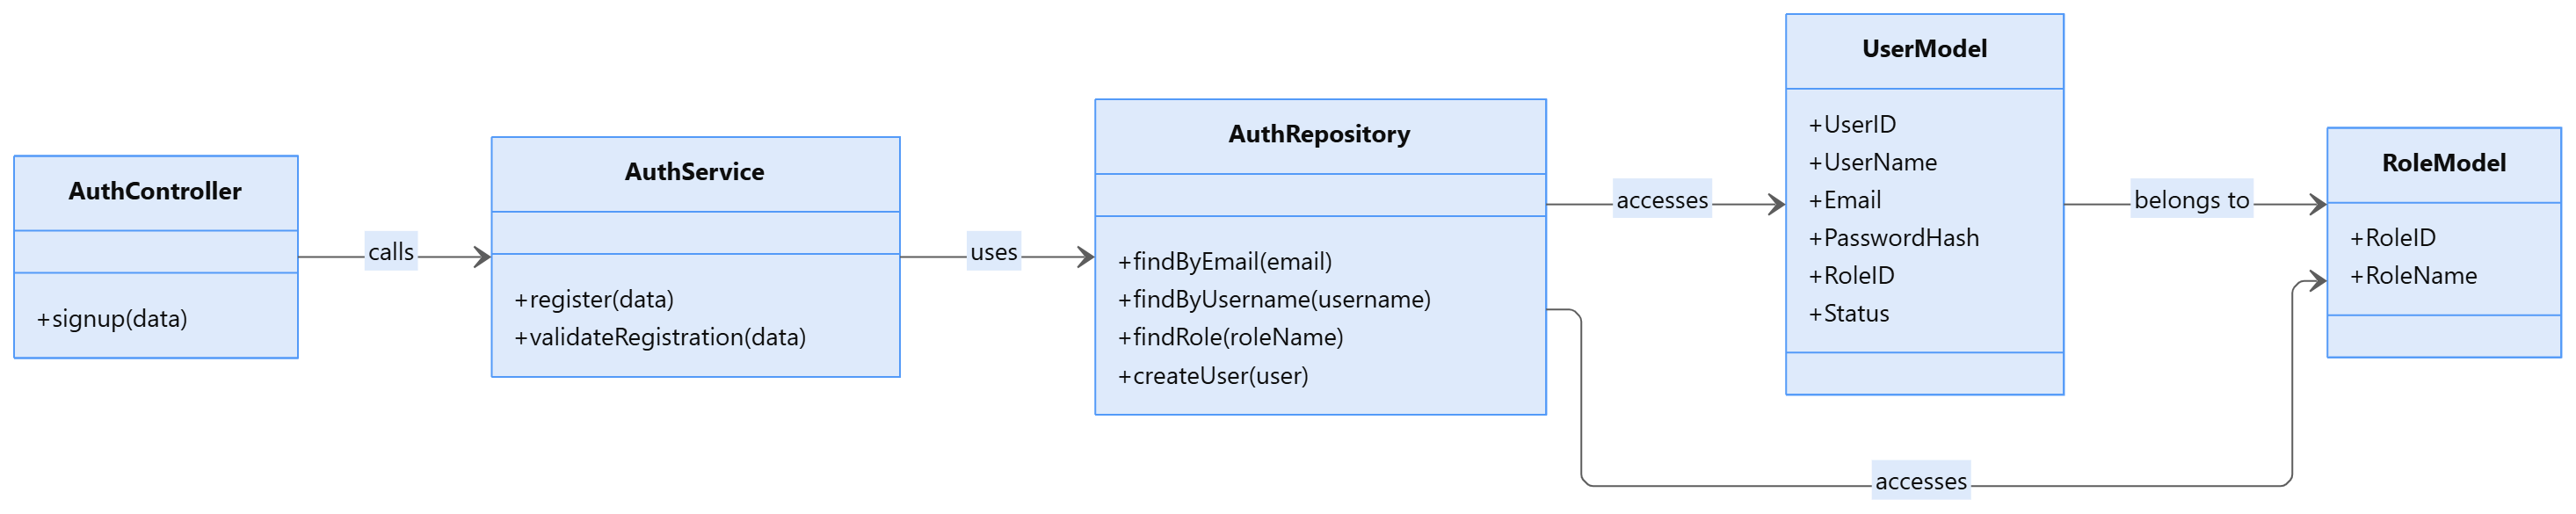
\includegraphics[width=1.1\textwidth]{images/12.png}
\end{figure}

\paragraph{Sequence Diagram}

\begin{figure}[H]
	\centering
	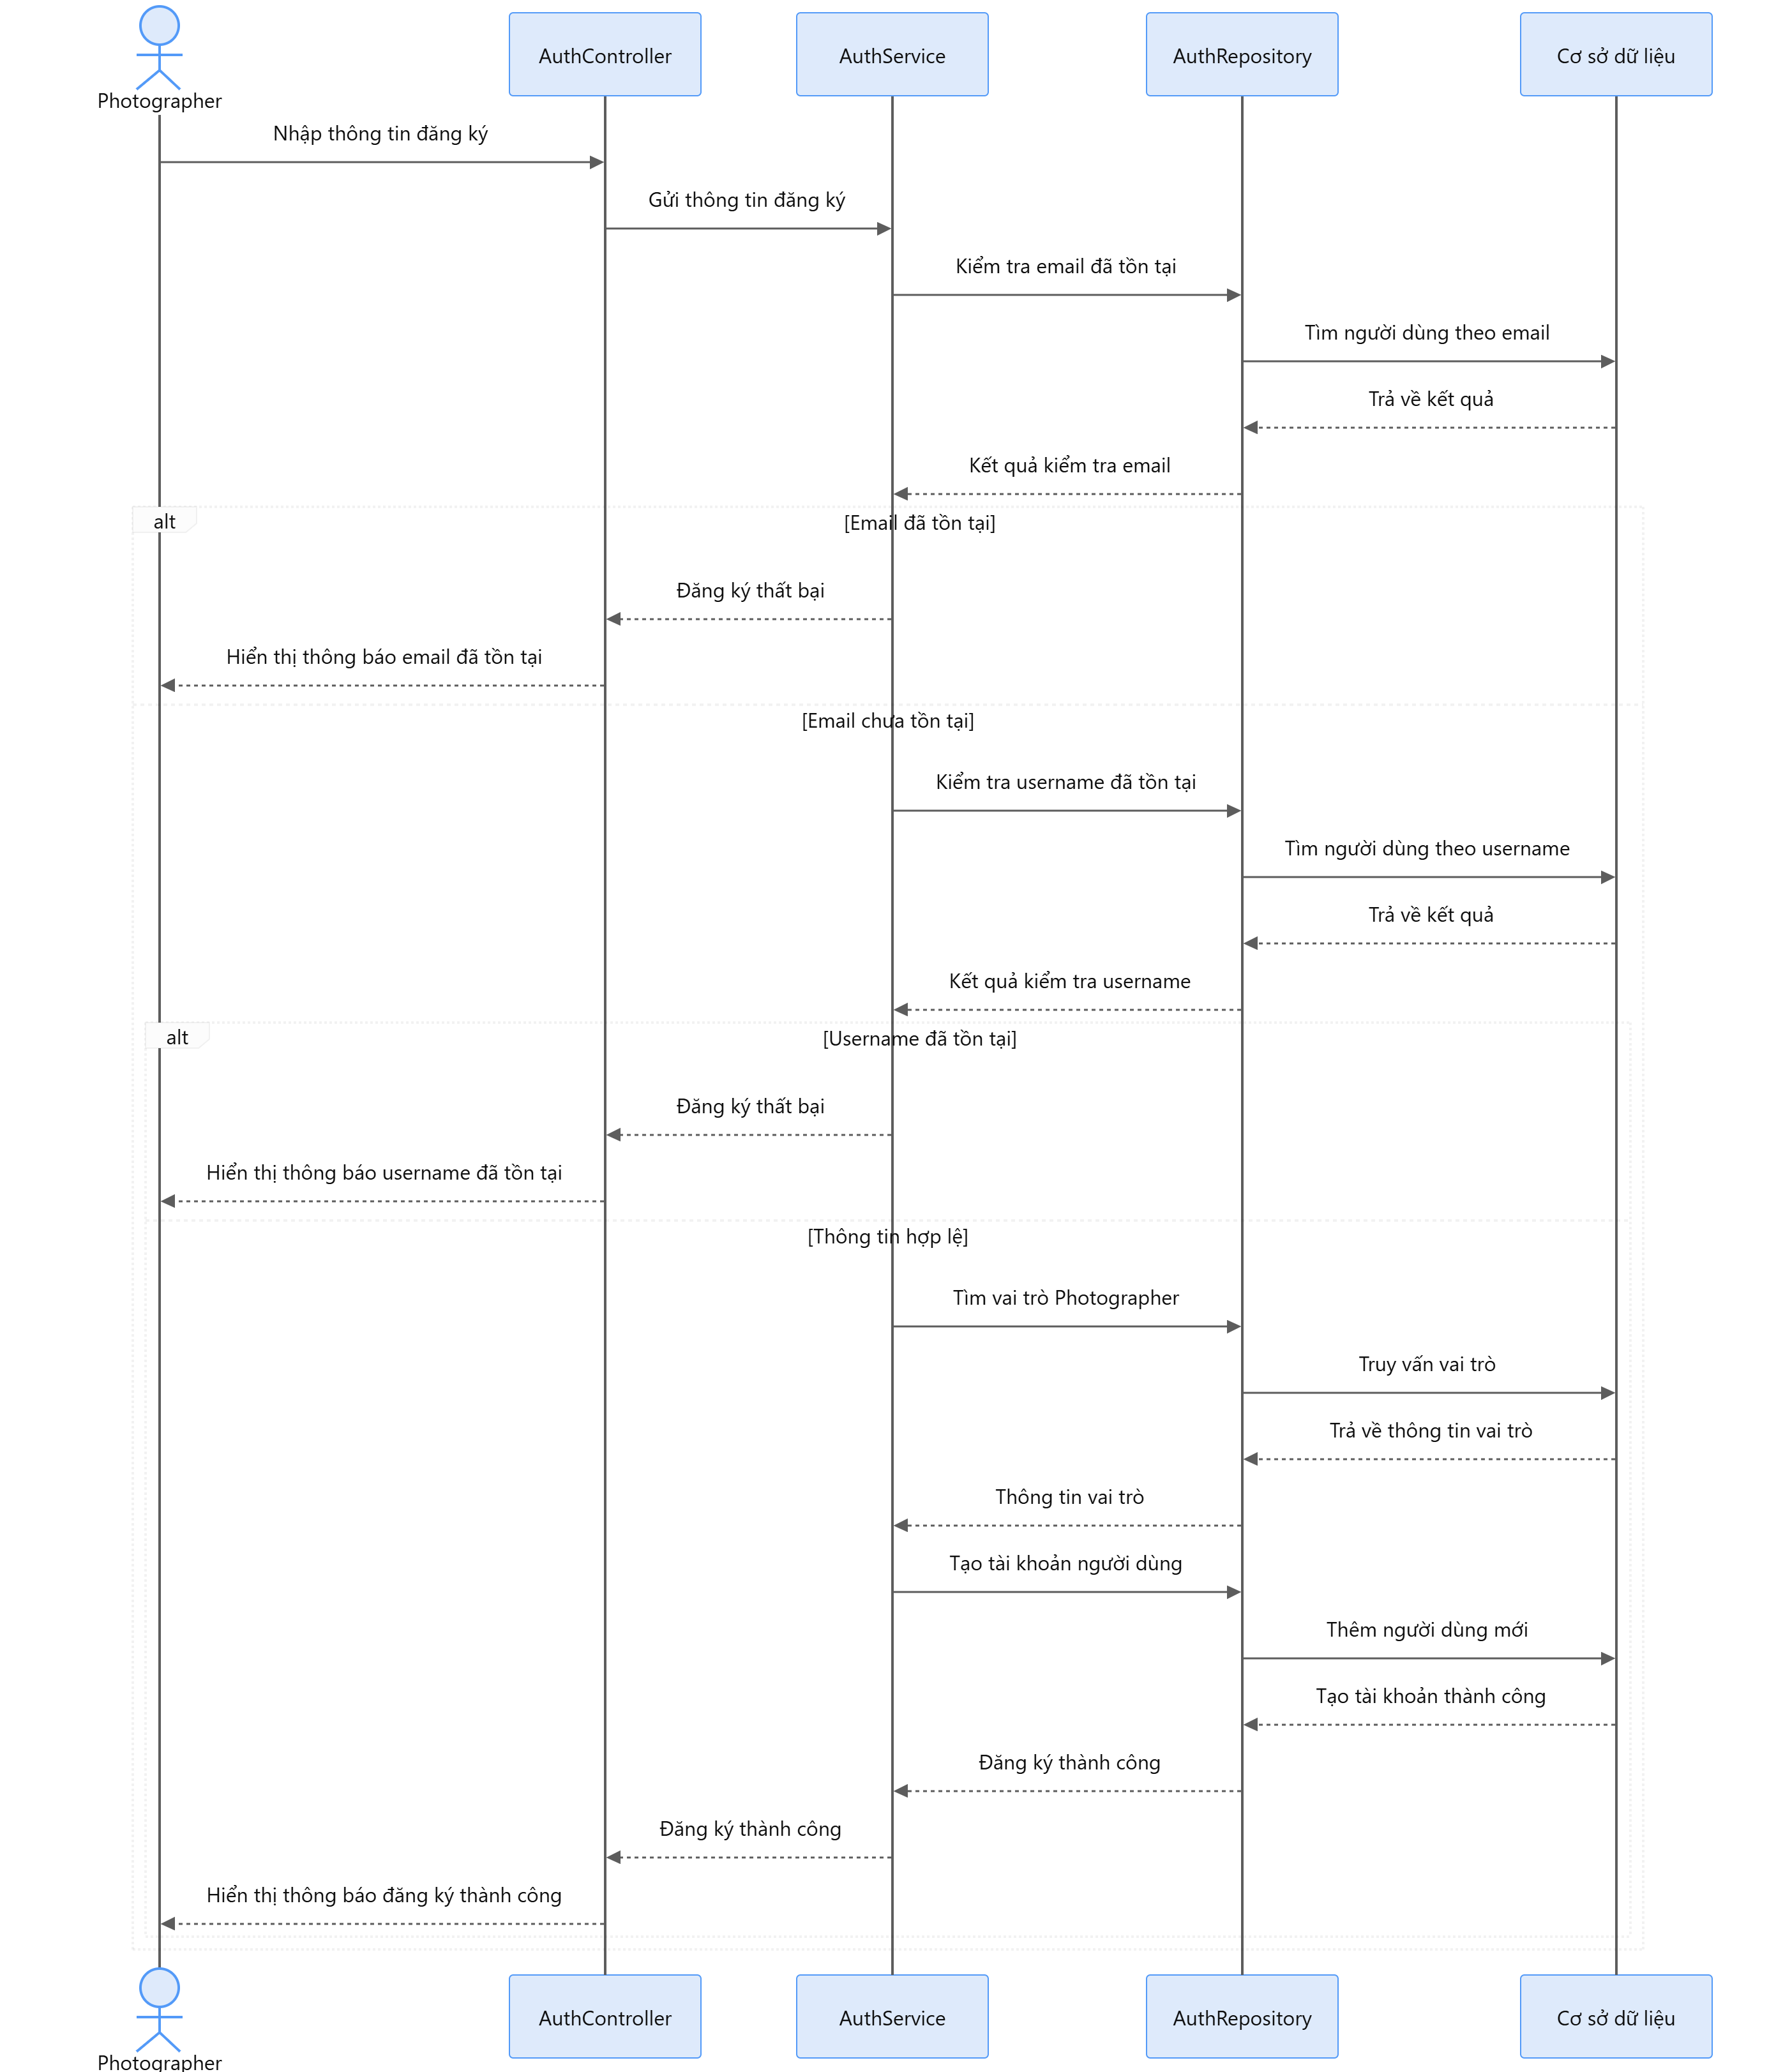
\includegraphics[width=1.1\textwidth]{images/13.png}
\end{figure}


\subsubsection{Đăng nhập}

\paragraph{Class Diagram}

\begin{figure}[H]
	\centering
	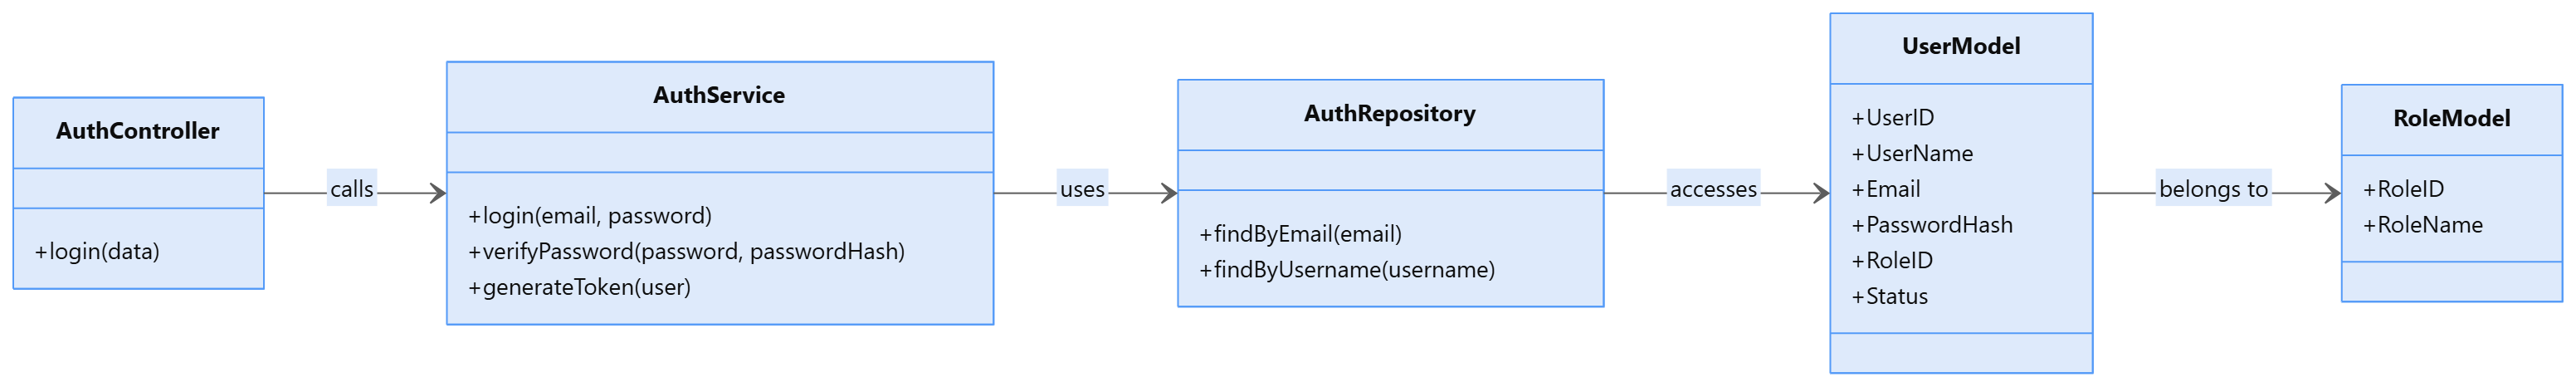
\includegraphics[width=1.1\textwidth]{images/14.png}
\end{figure}

\paragraph{Sequence Diagram}

\begin{figure}[H]
	\centering
	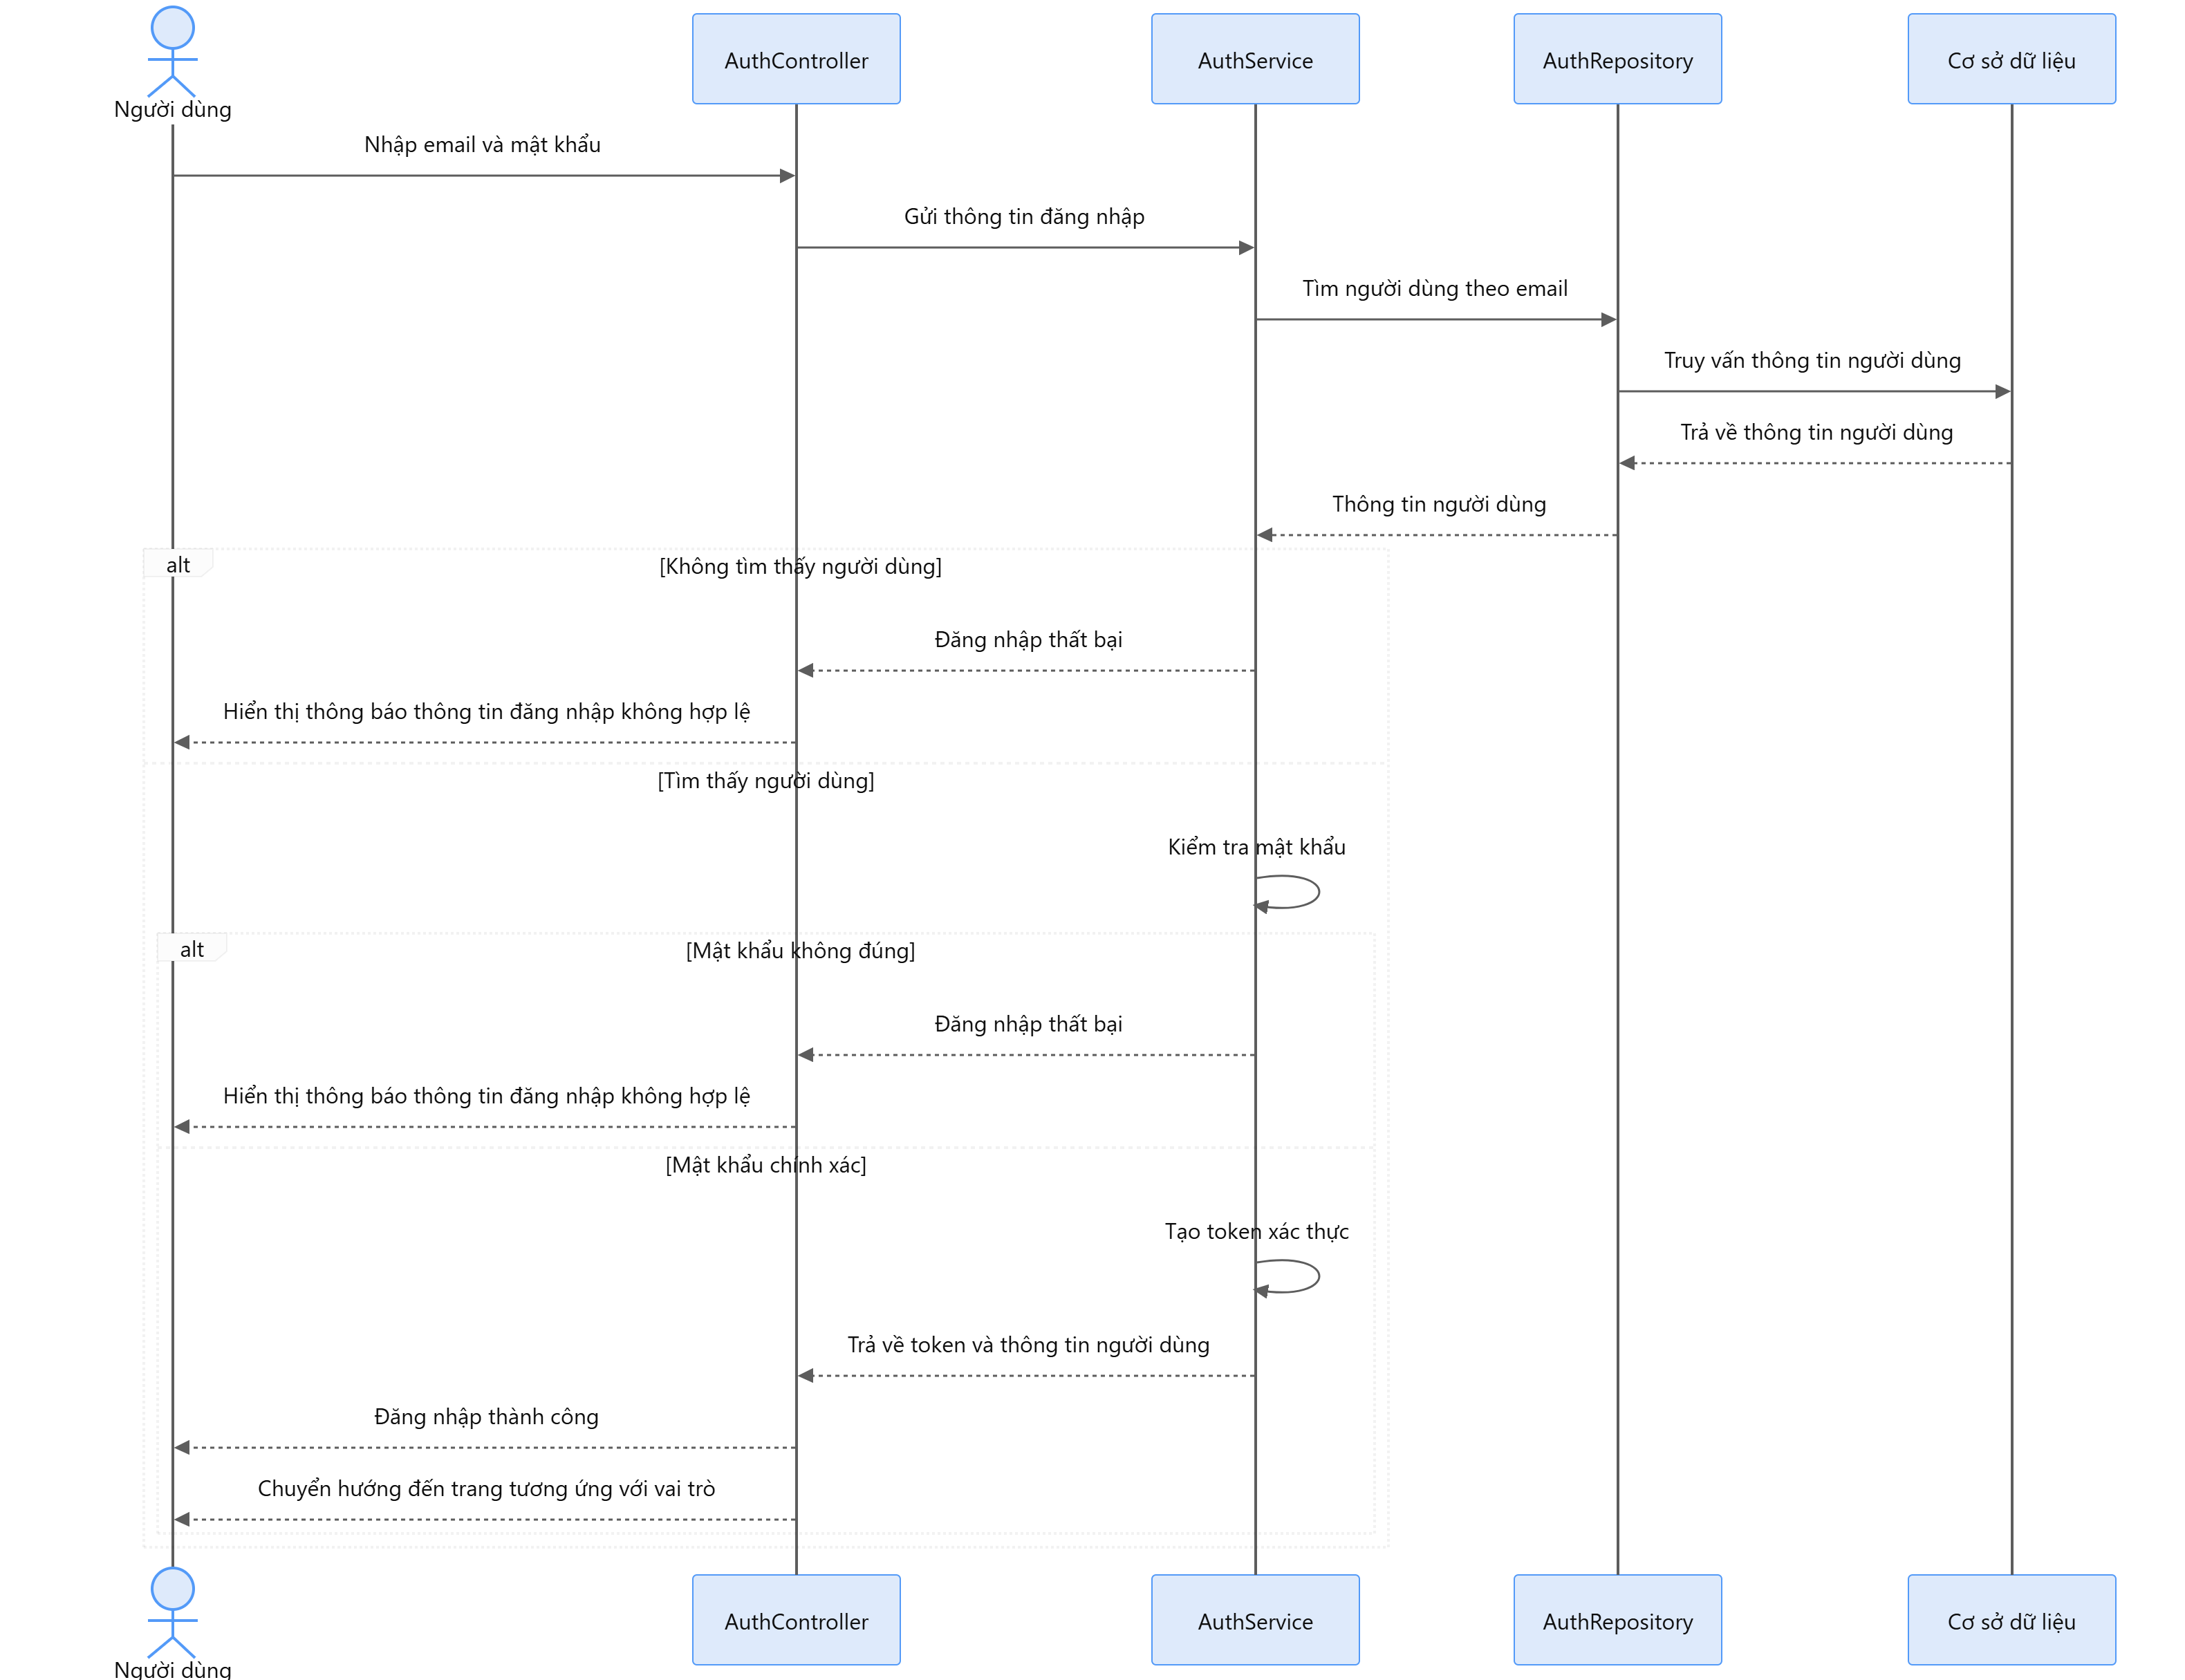
\includegraphics[width=1.1\textwidth]{images/15.png}
\end{figure}


\subsubsection{Quên mật khẩu}

\paragraph{Class Diagram}

\begin{figure}[H]
	\centering
	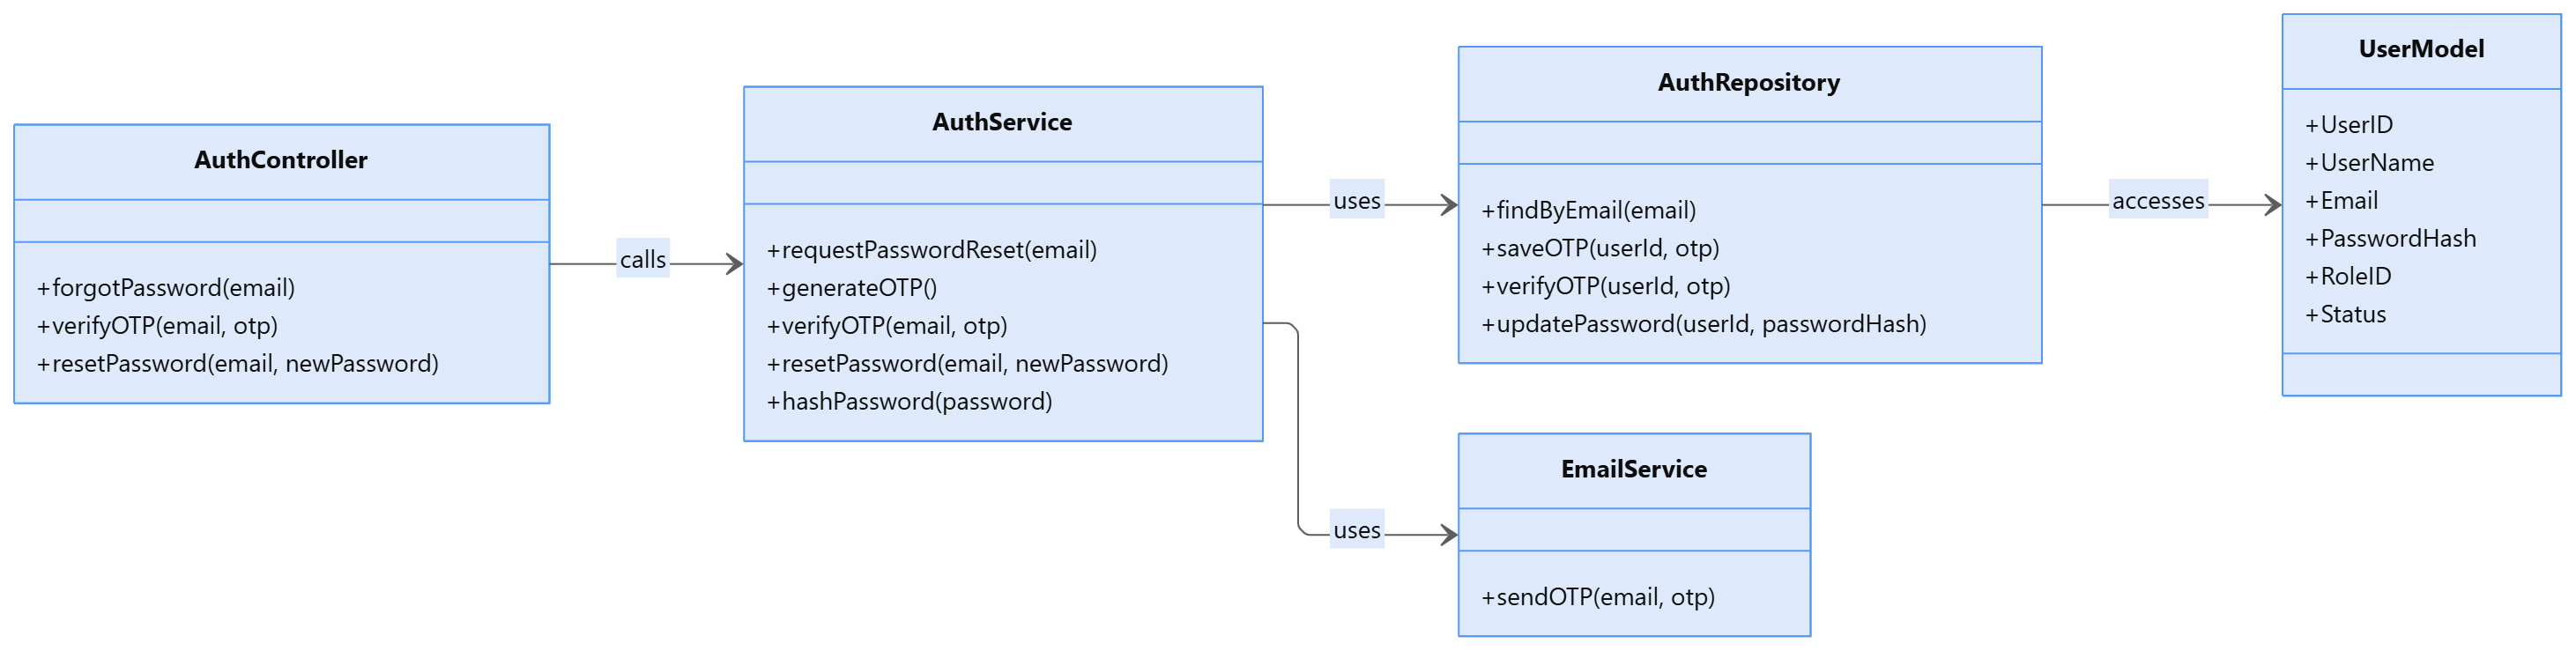
\includegraphics[width=1.1\textwidth]{images/16.png}
\end{figure}

\paragraph{Sequence Diagram}

\begin{figure}[H]
	\centering
	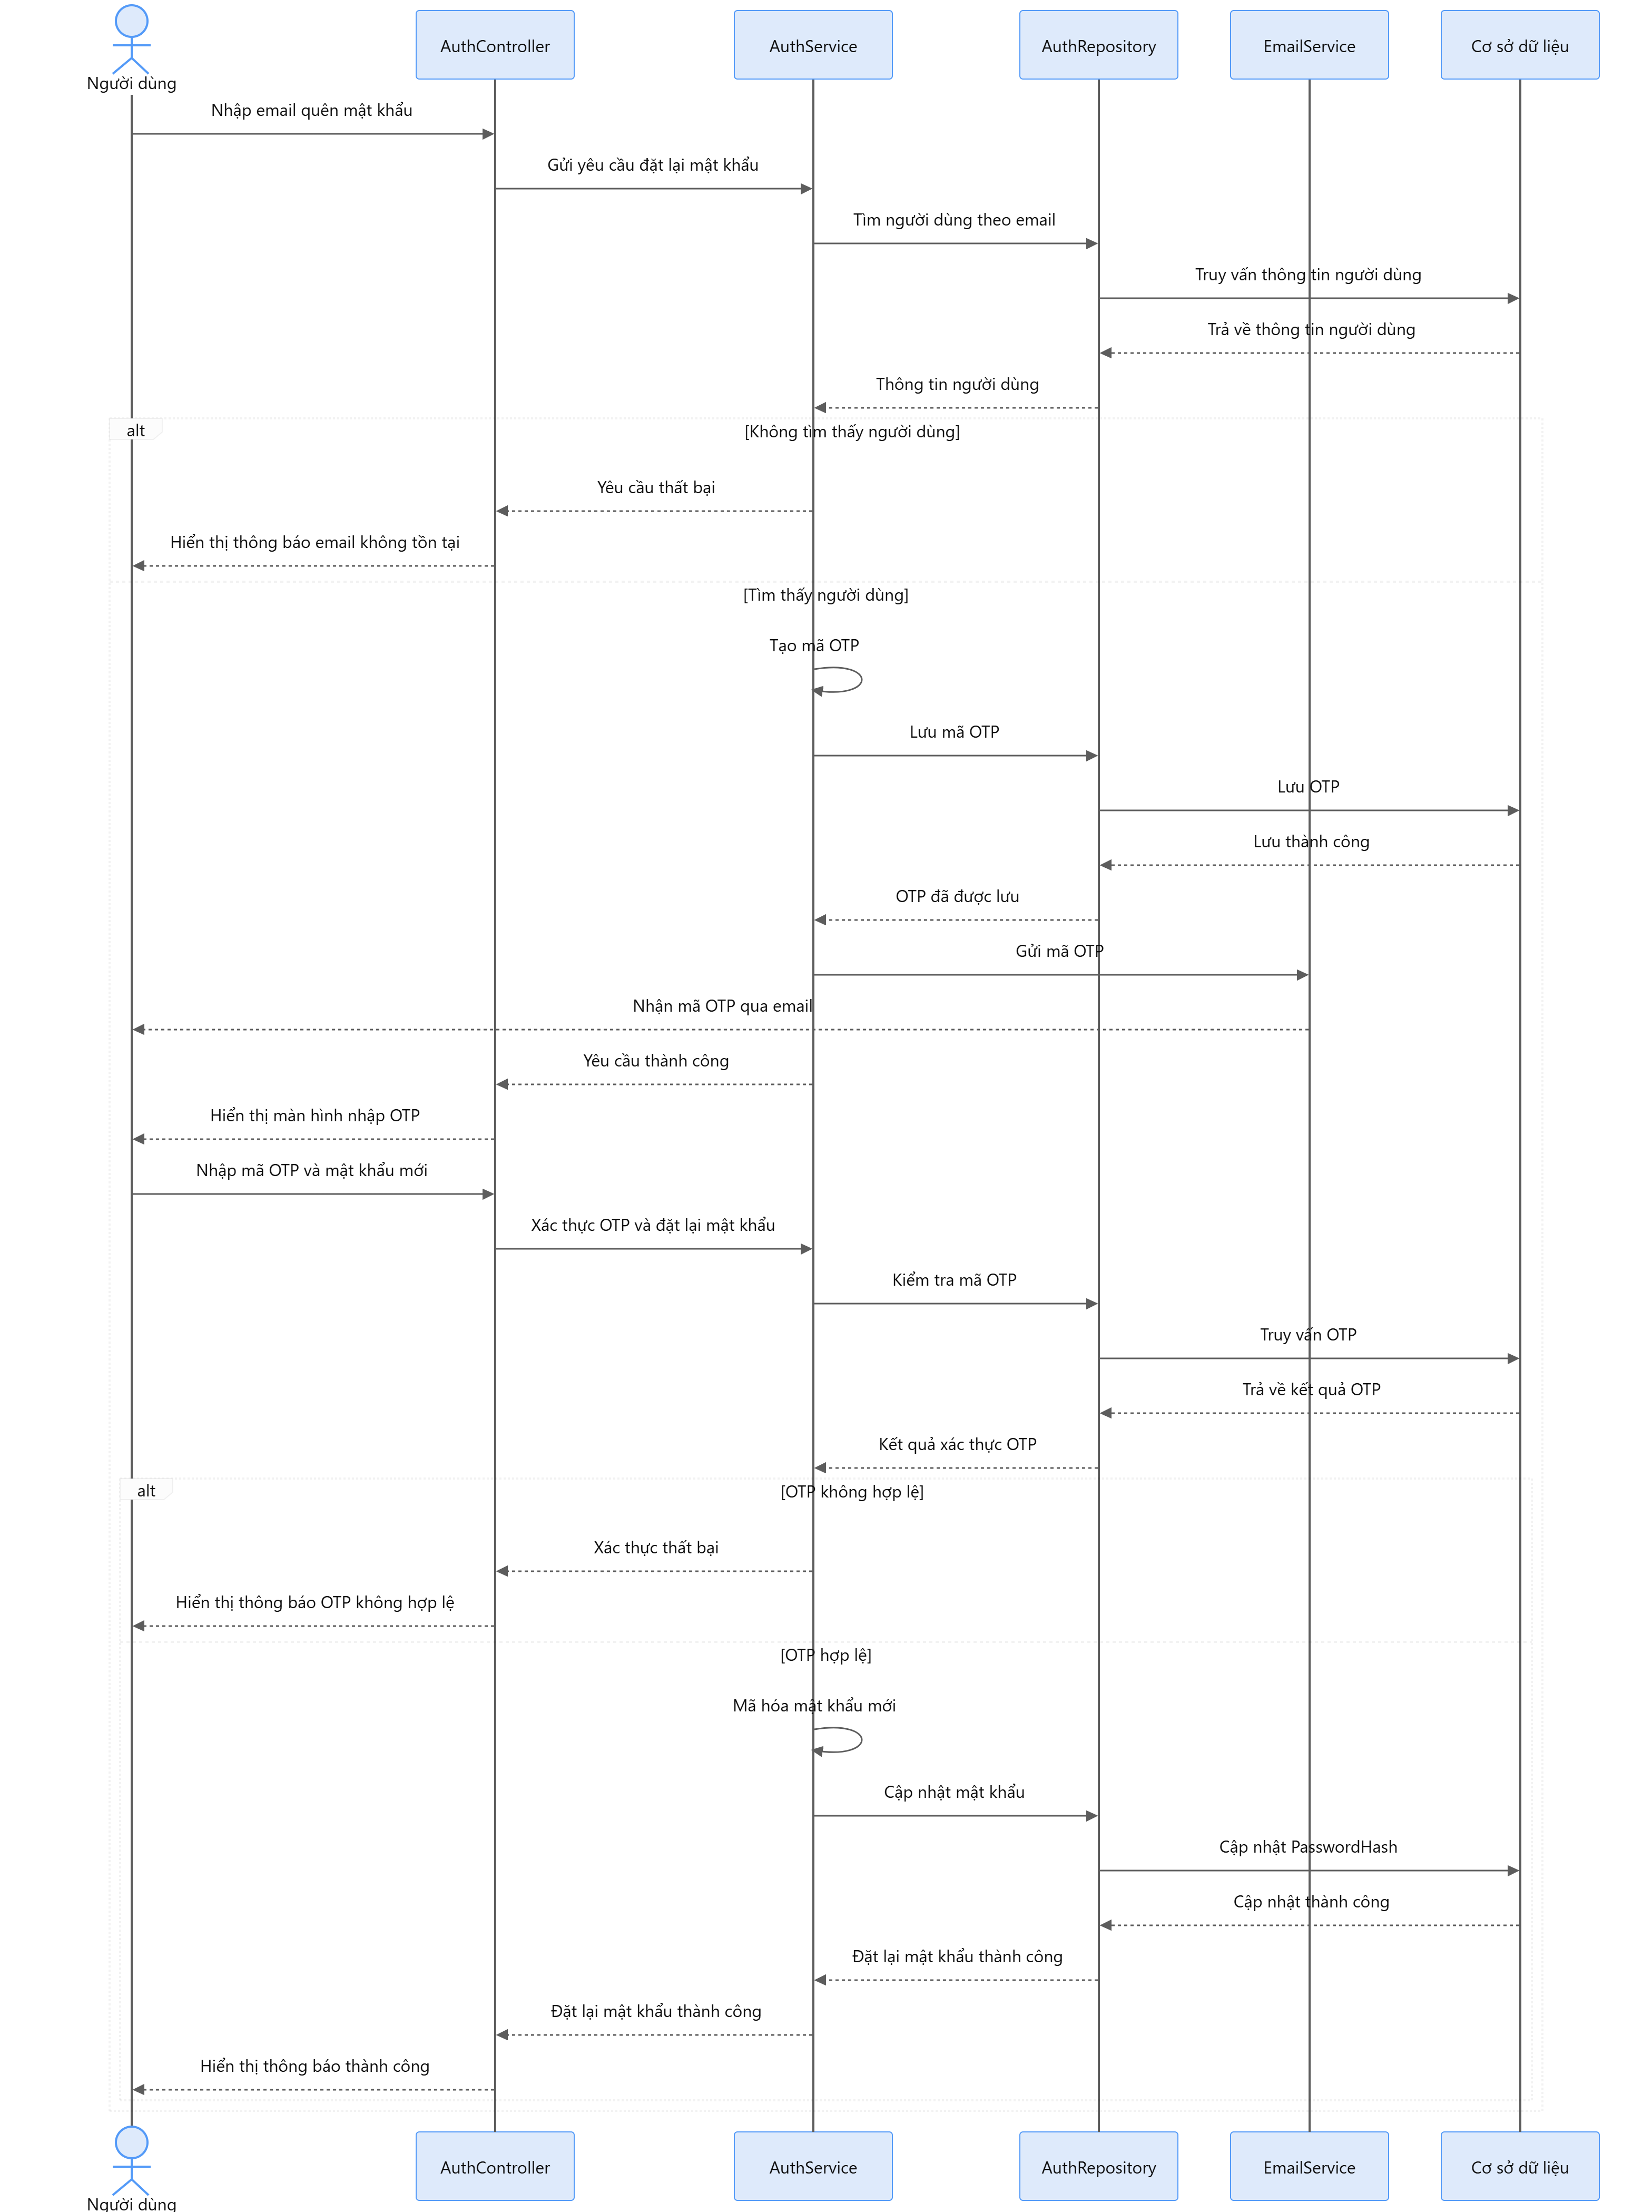
\includegraphics[width=1.1\textwidth]{images/17.png}
\end{figure}


\subsubsection{Đổi mật khẩu}

\paragraph{Class Diagram}

\begin{figure}[H]
	\centering
	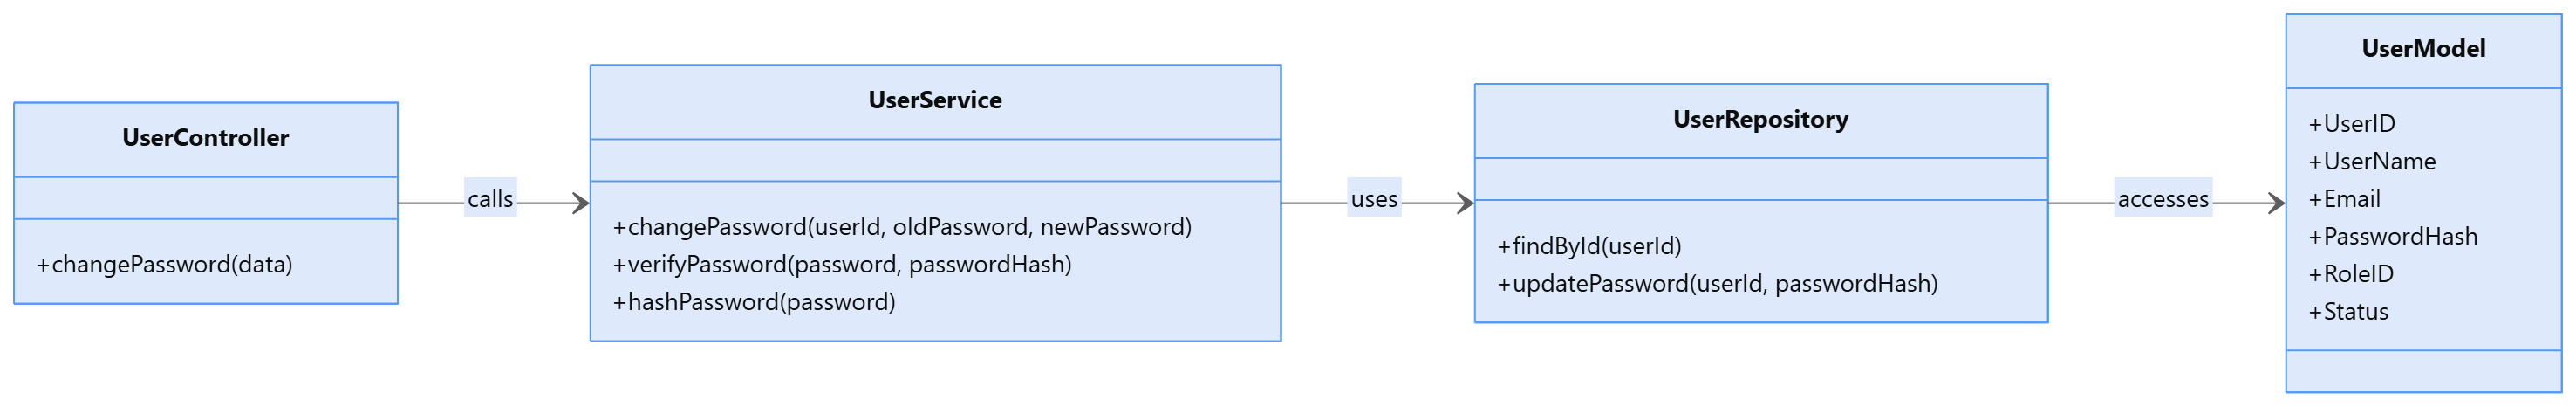
\includegraphics[width=1.1\textwidth]{images/18.png}
\end{figure}

\paragraph{Sequence Diagram}

\begin{figure}[H]
	\centering
	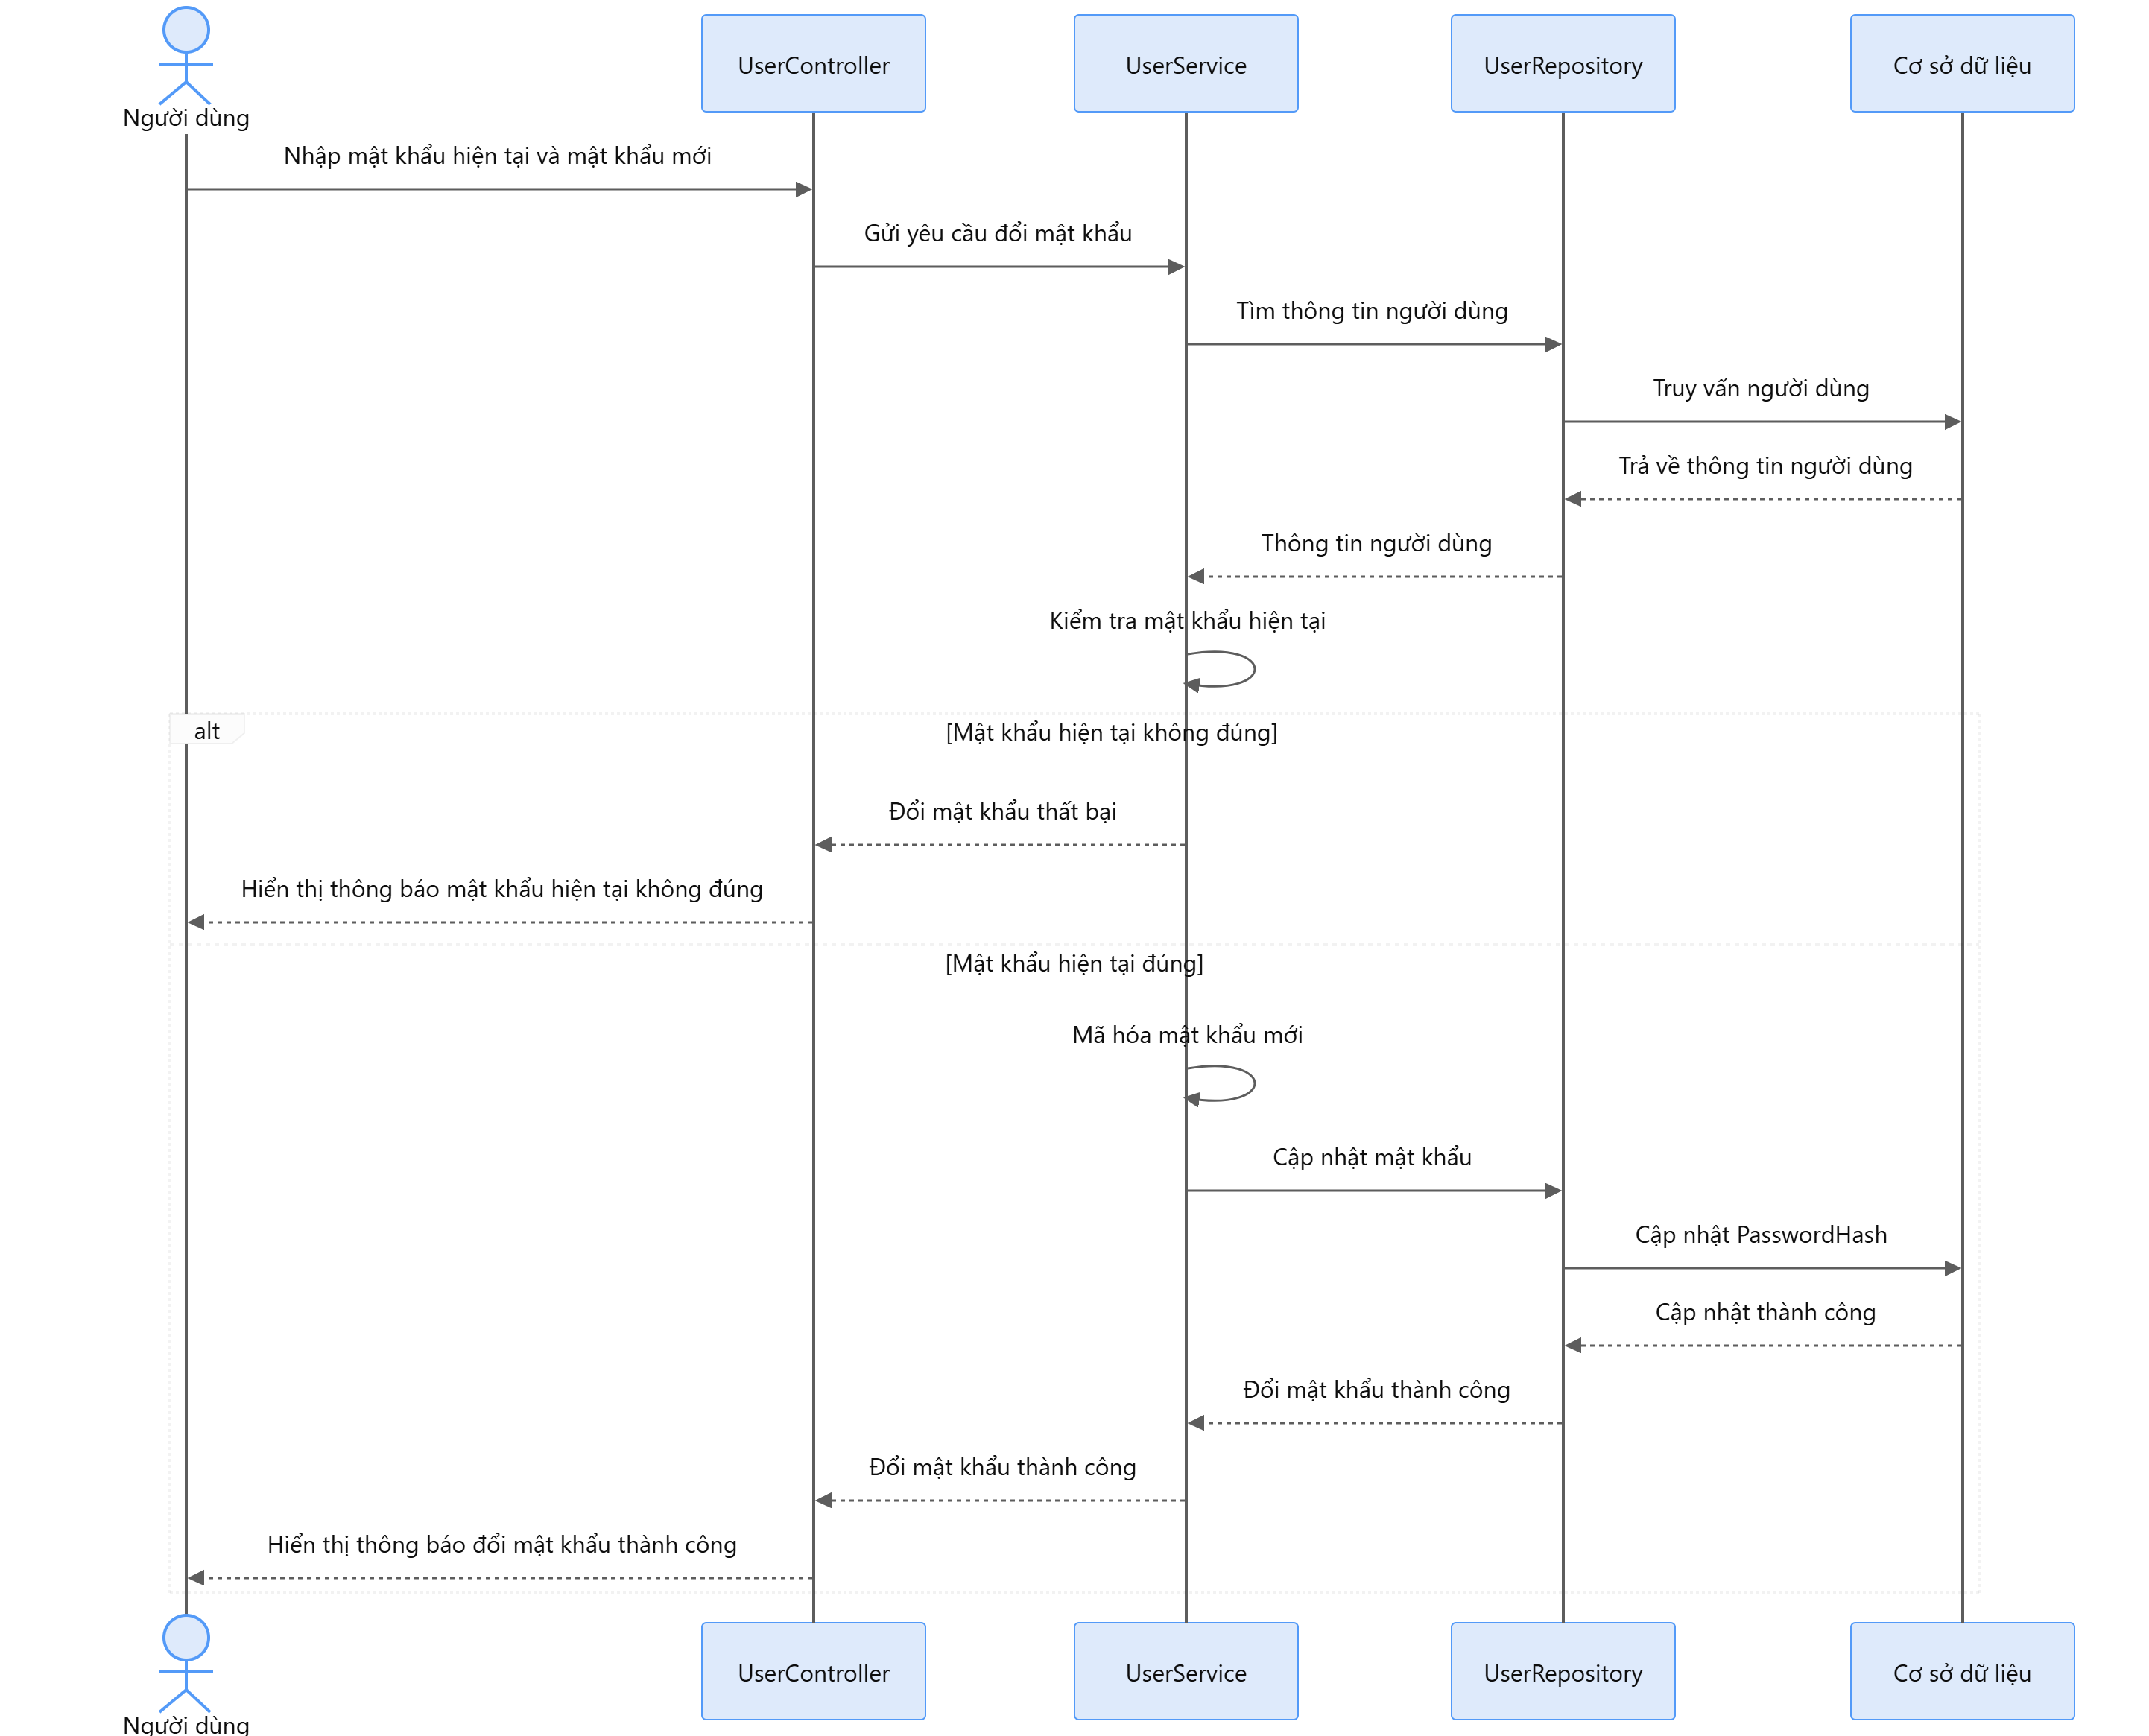
\includegraphics[width=1.1\textwidth]{images/19.png}
\end{figure}


% =========================================================
% 3.2 Photographer Management Module
% =========================================================

\subsection{Photographer Management Module}

\subsubsection{Quản lý hồ sơ}

\paragraph{Class Diagram}

\begin{figure}[H]
	\centering
	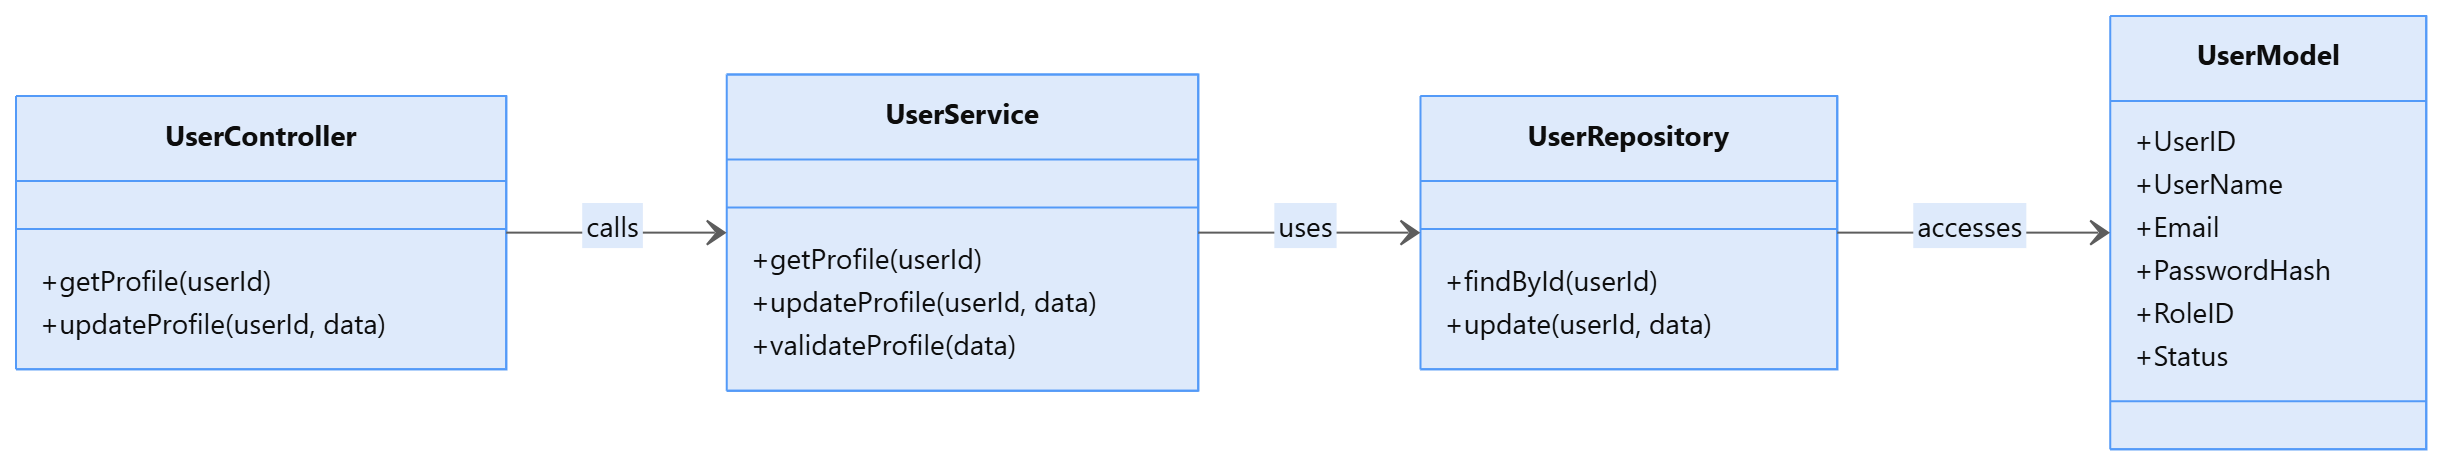
\includegraphics[width=1.1\textwidth]{images/20.png}
\end{figure}

\paragraph{Sequence Diagram}

\begin{figure}[H]
	\centering
	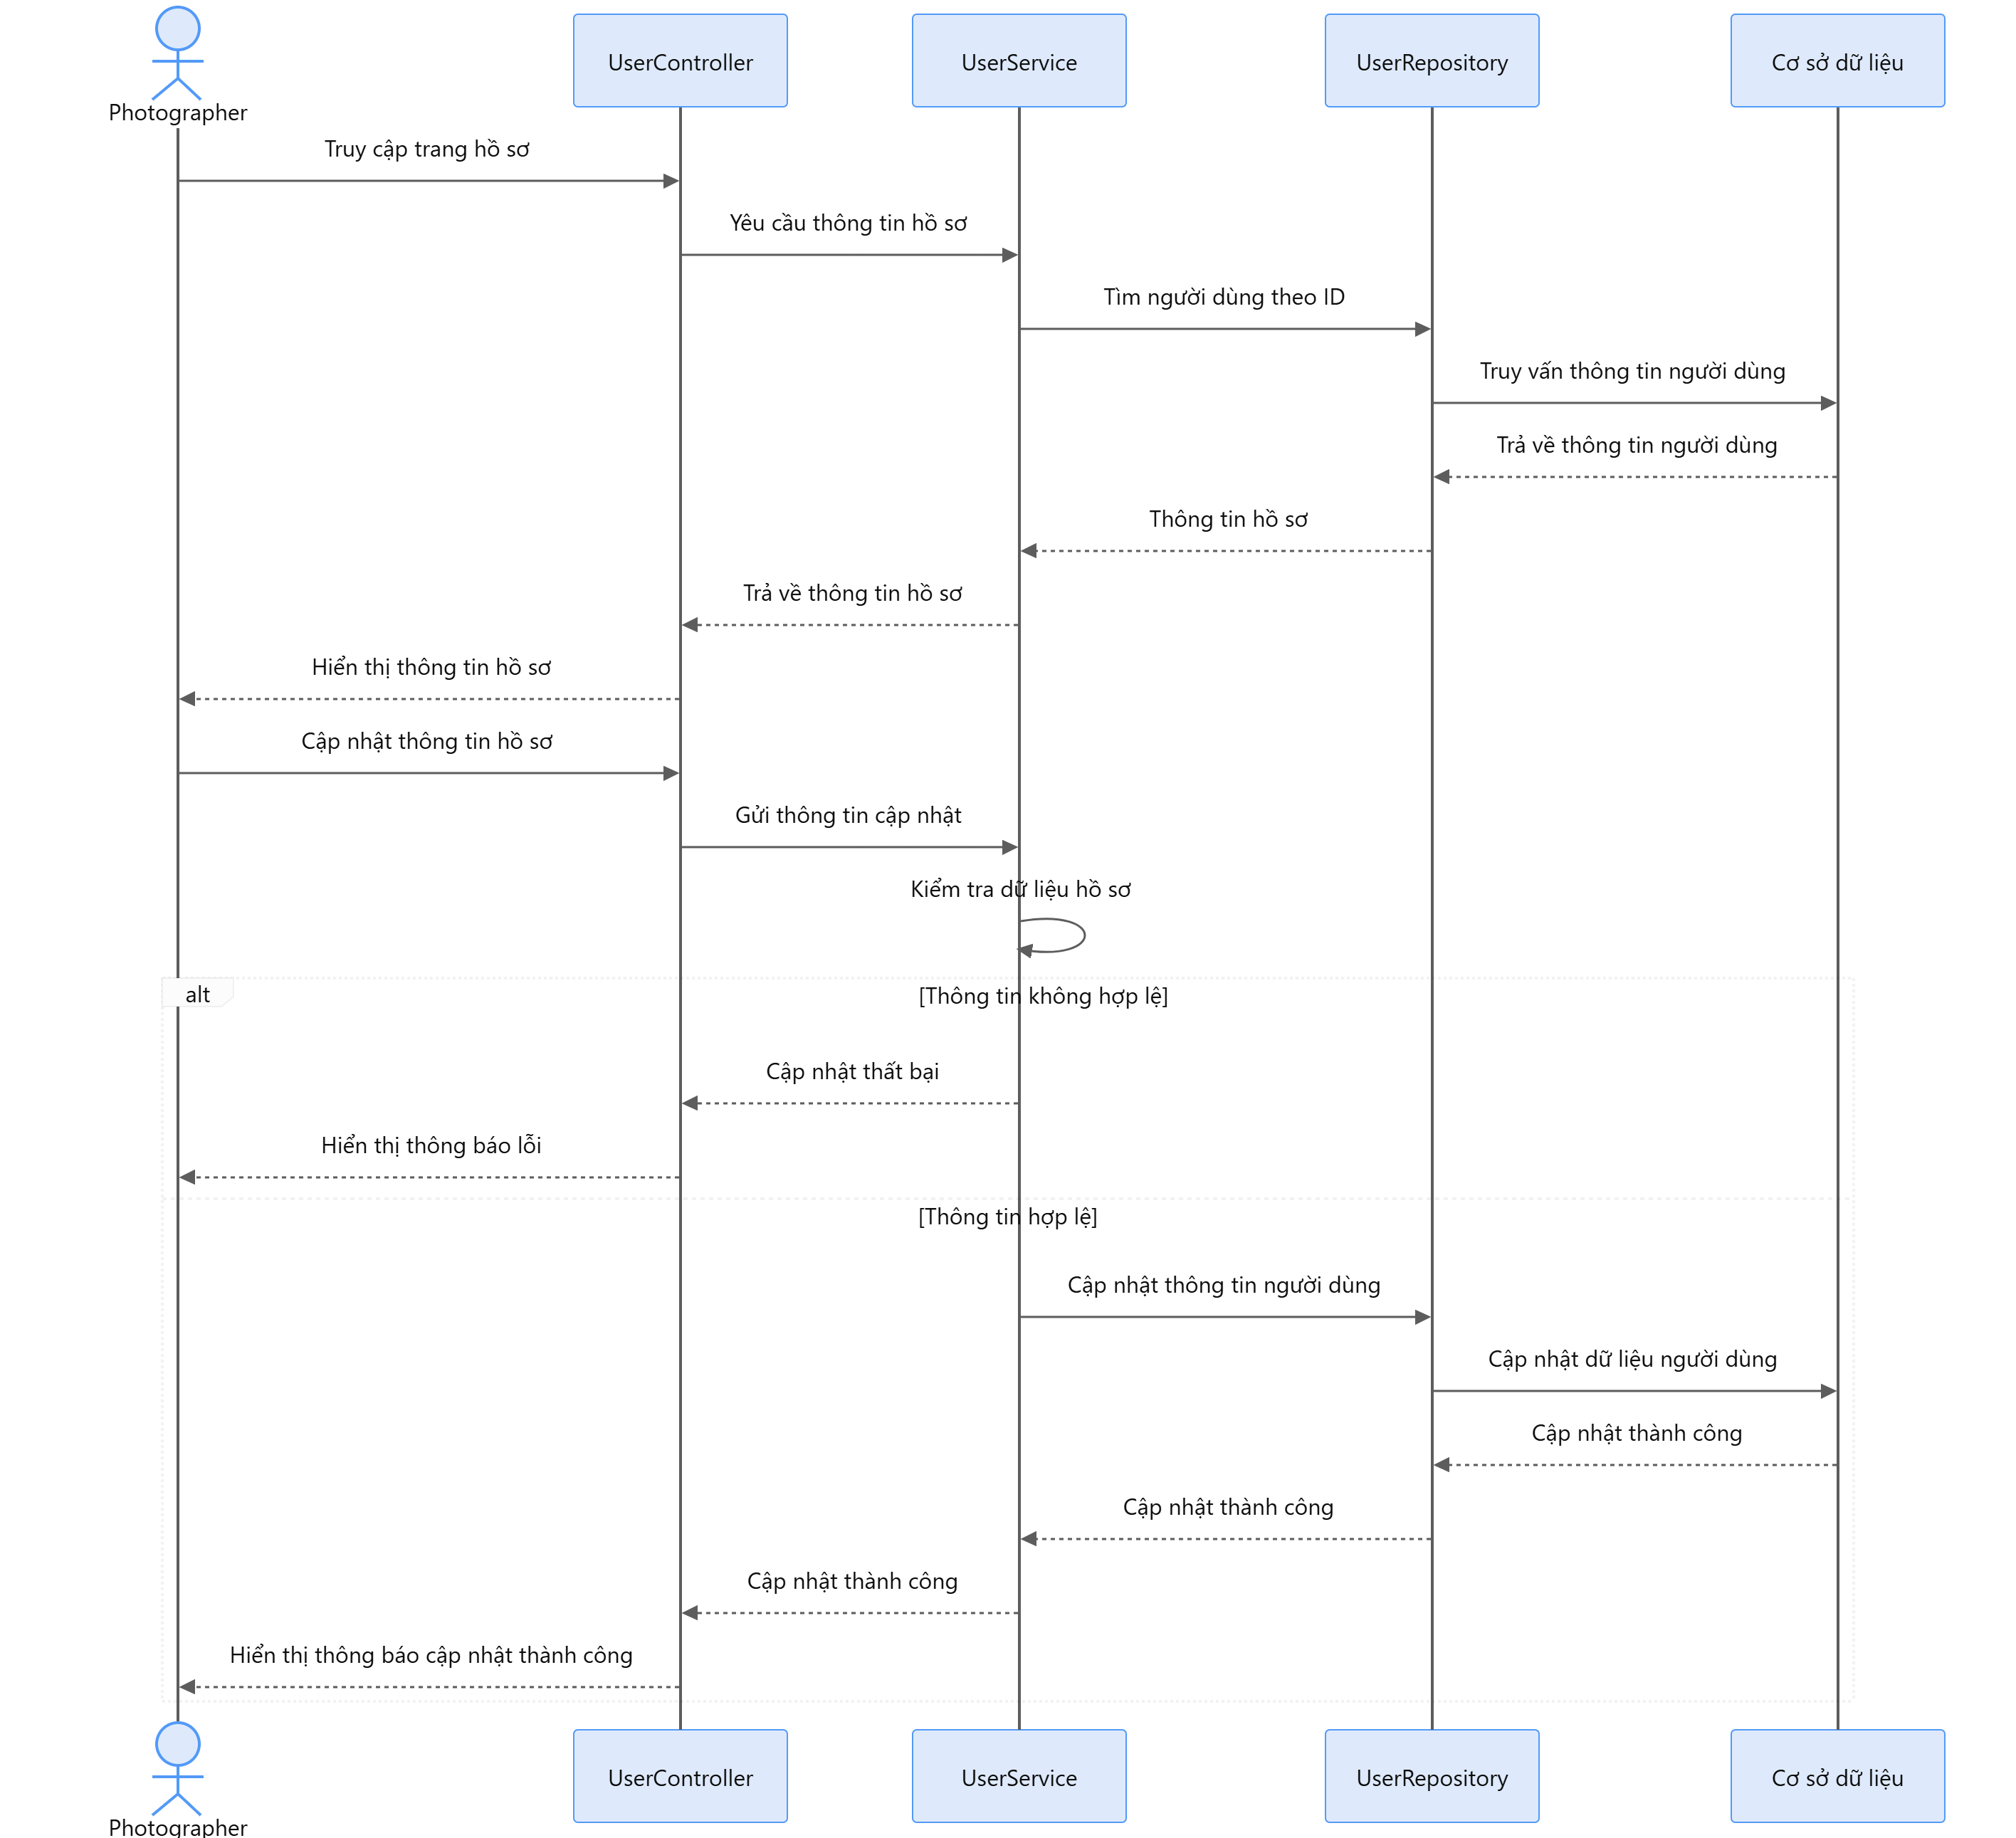
\includegraphics[width=1.1\textwidth]{images/21.png}
\end{figure}


% =========================================================
% 3.3 Service Search and Discovery Module
% =========================================================

\subsection{Service Search and Discovery Module}

\subsubsection{Tìm kiếm Creative Space}

\paragraph{Class Diagram}

\begin{figure}[H]
	\centering
	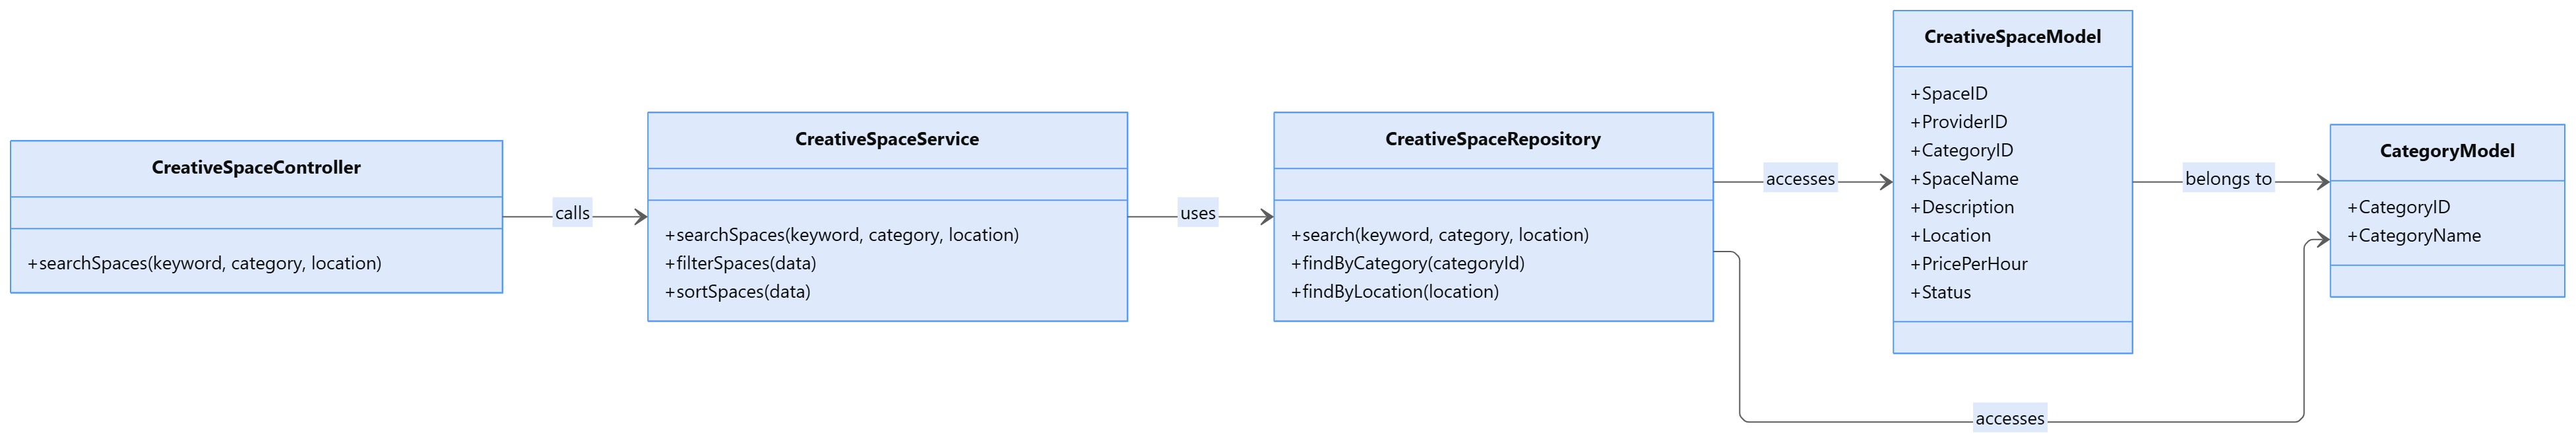
\includegraphics[width=1.1\textwidth]{images/22.png}
\end{figure}

\paragraph{Sequence Diagram}

\begin{figure}[H]
	\centering
	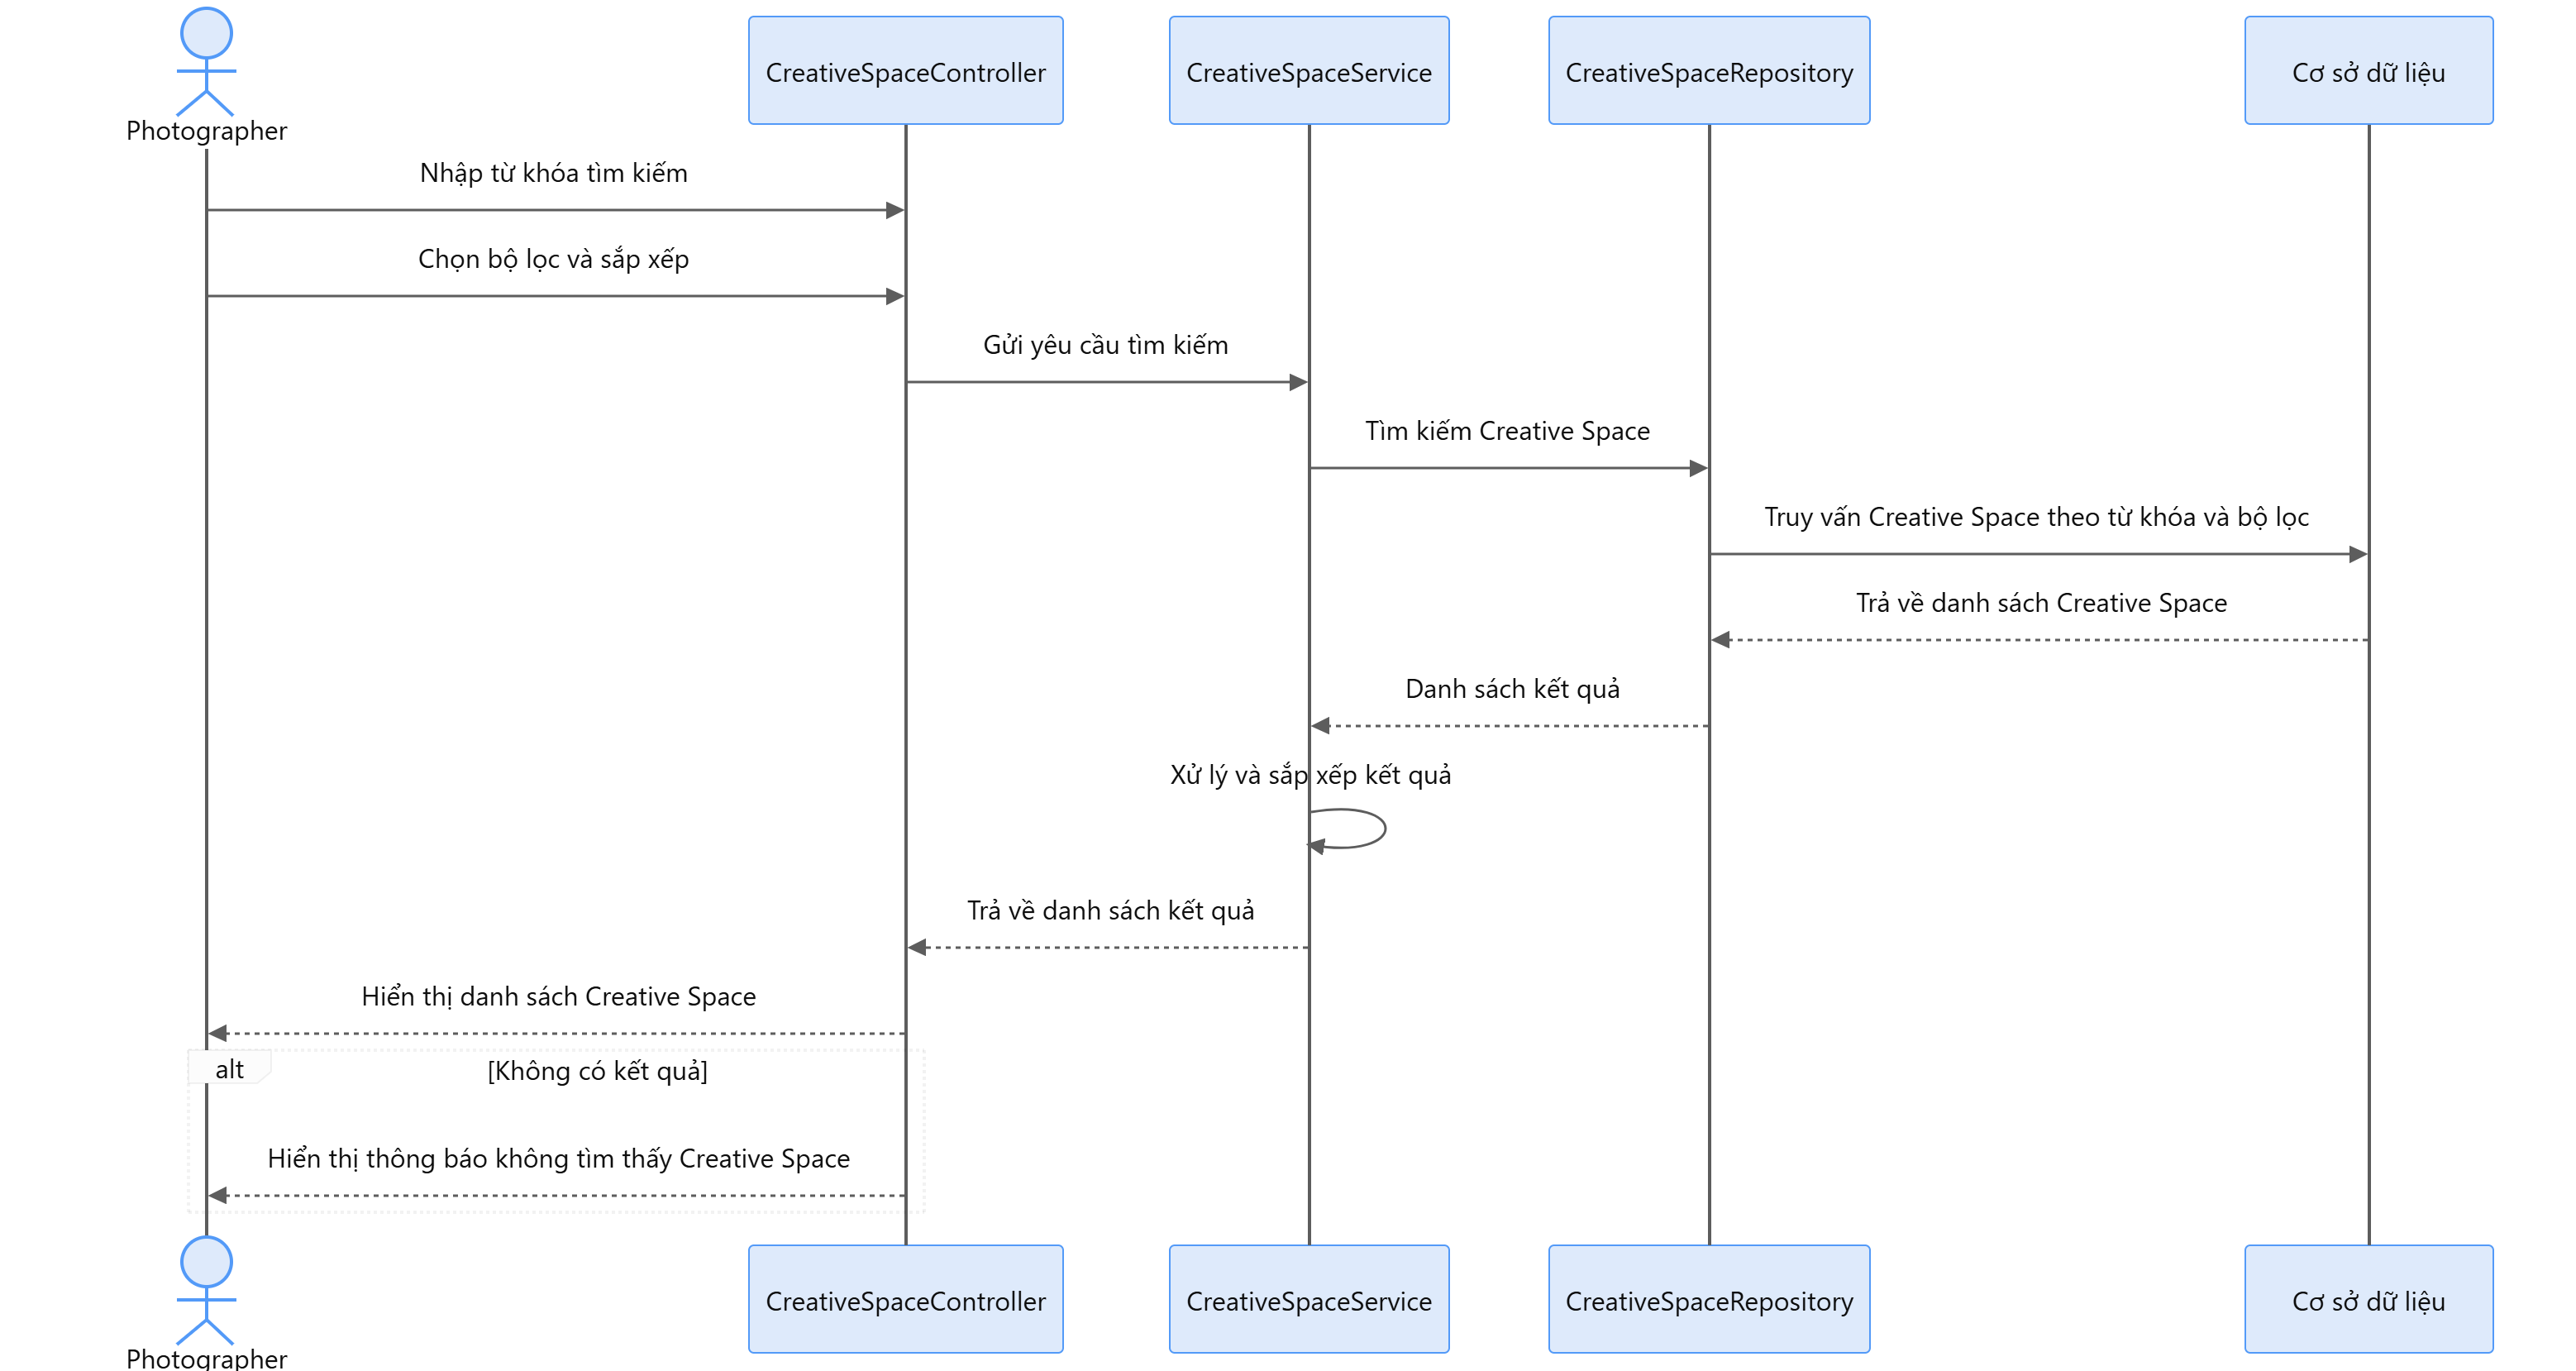
\includegraphics[width=1.1\textwidth]{images/23.png}
\end{figure}


\subsubsection{Xem chi tiết Creative Space}

\paragraph{Class Diagram}

\begin{figure}[H]
	\centering
	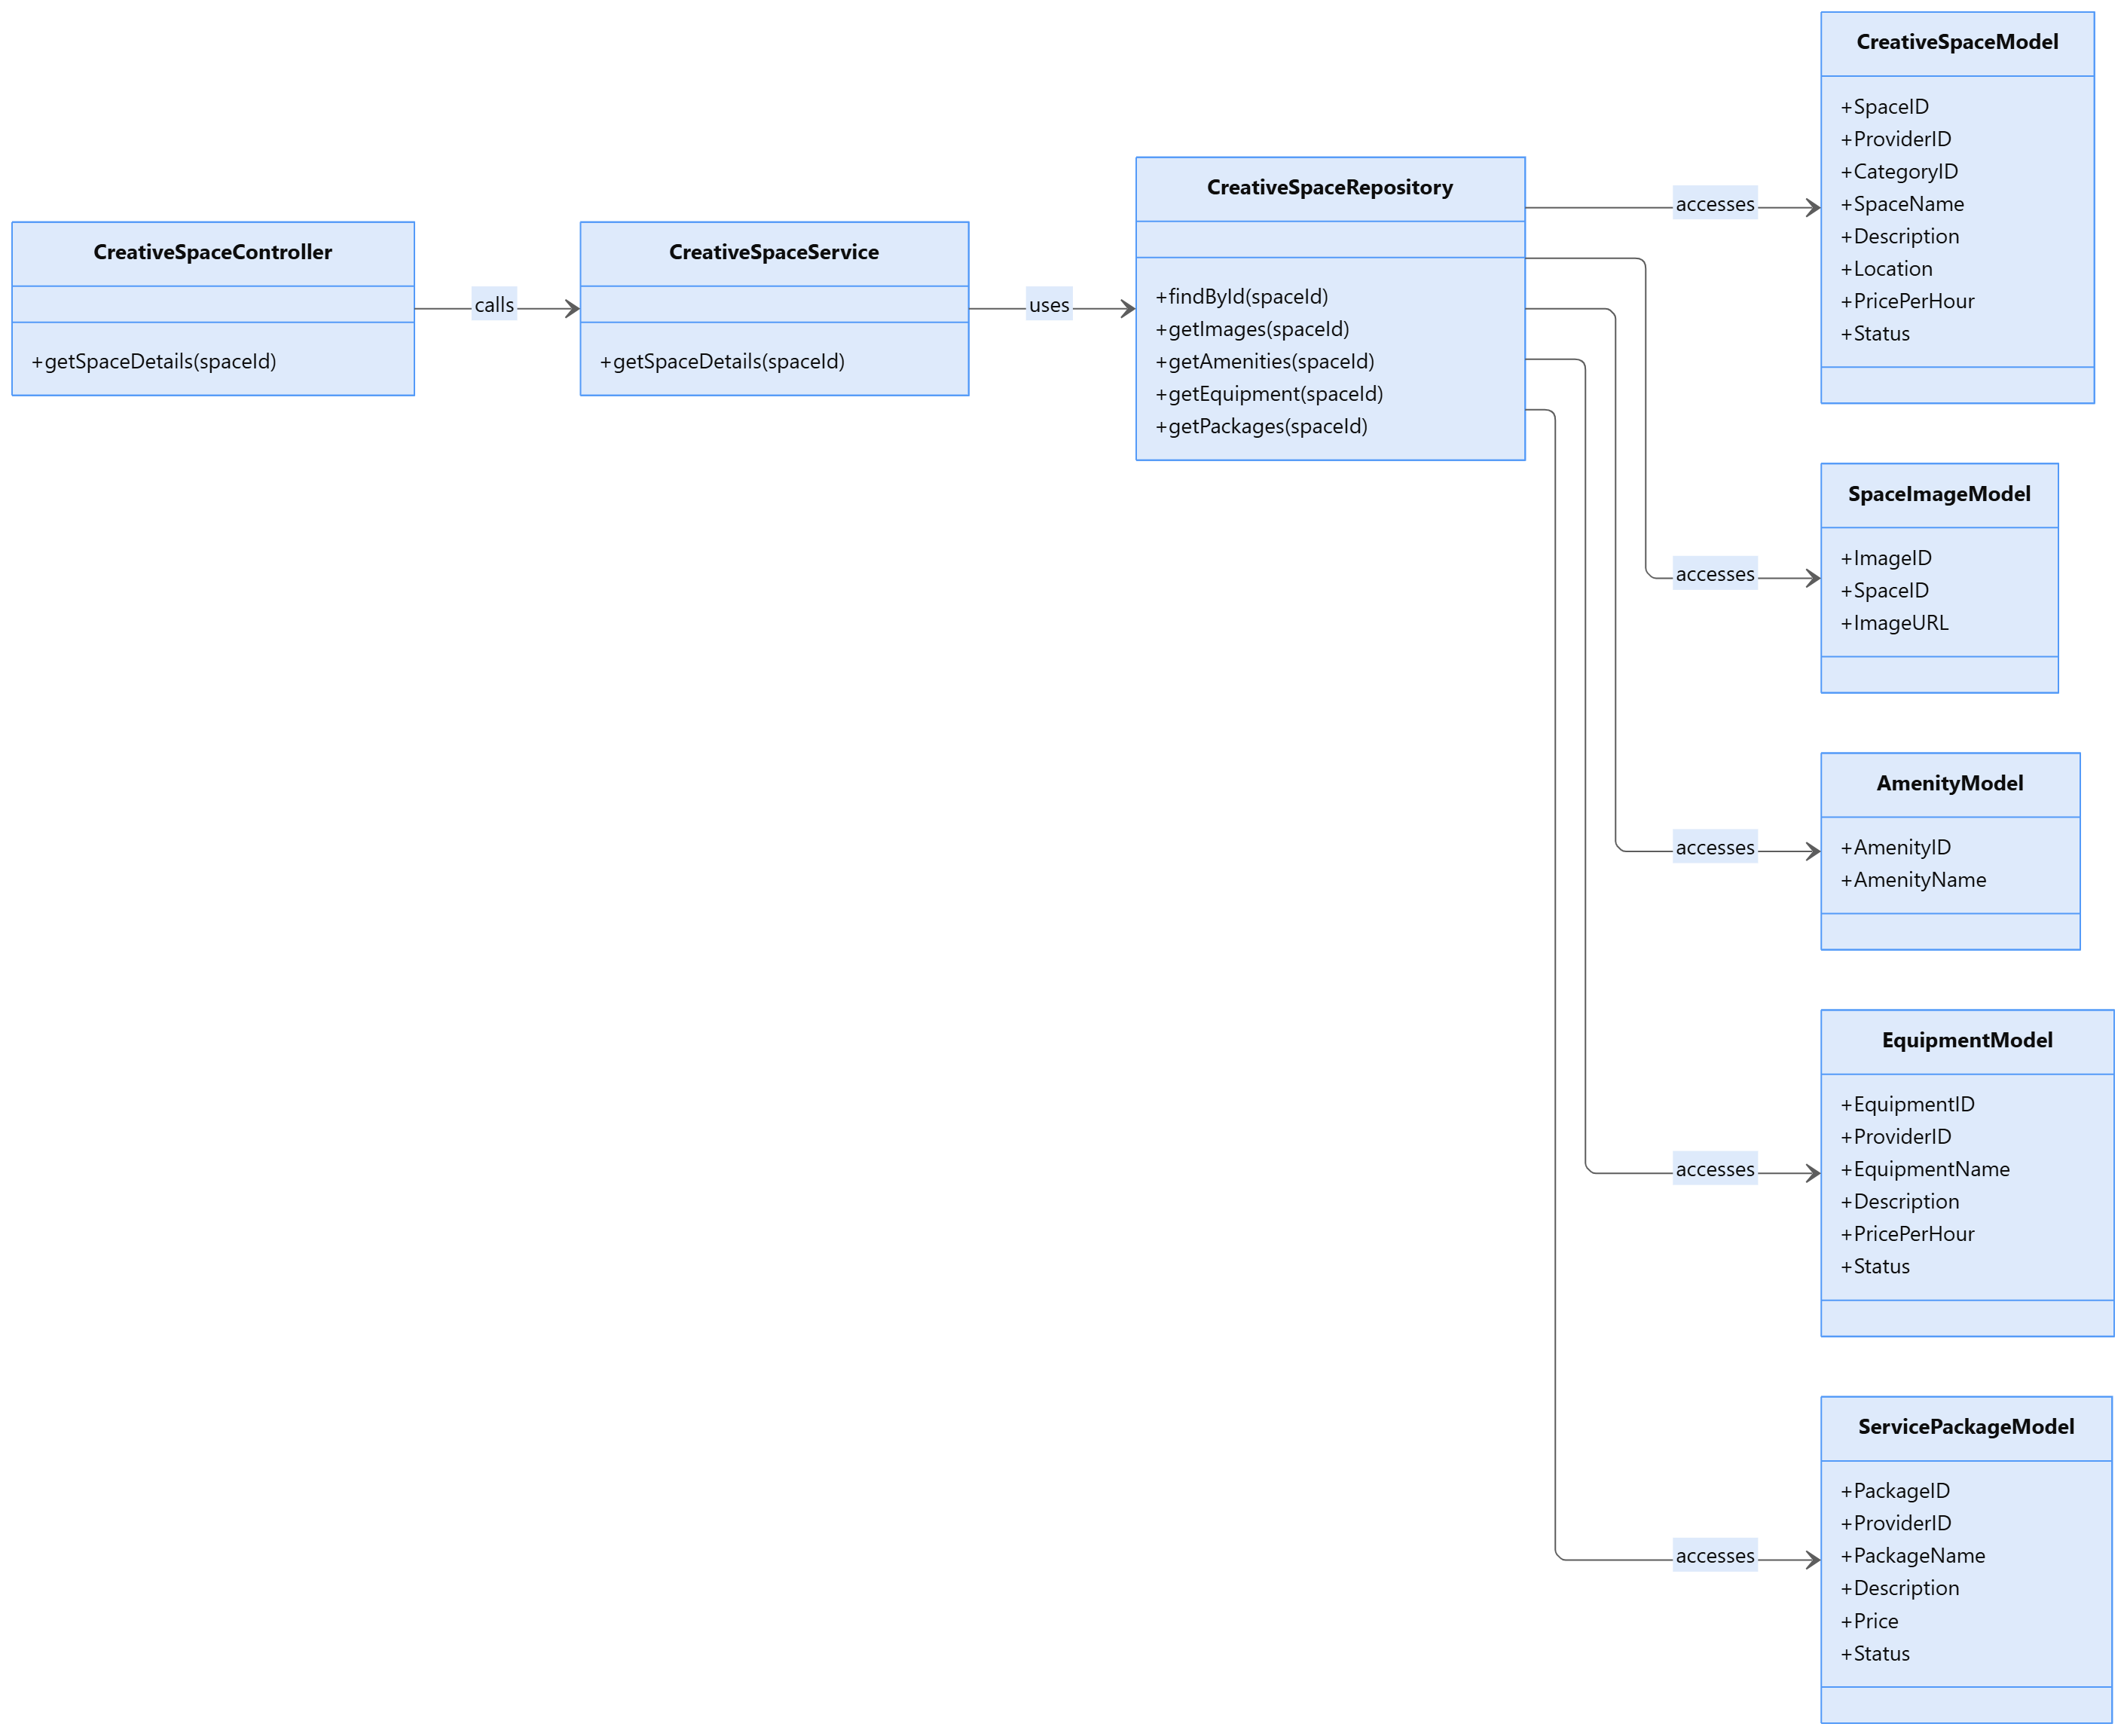
\includegraphics[width=1.1\textwidth]{images/24.png}
\end{figure}

\paragraph{Sequence Diagram}

\begin{figure}[H]
	\centering
	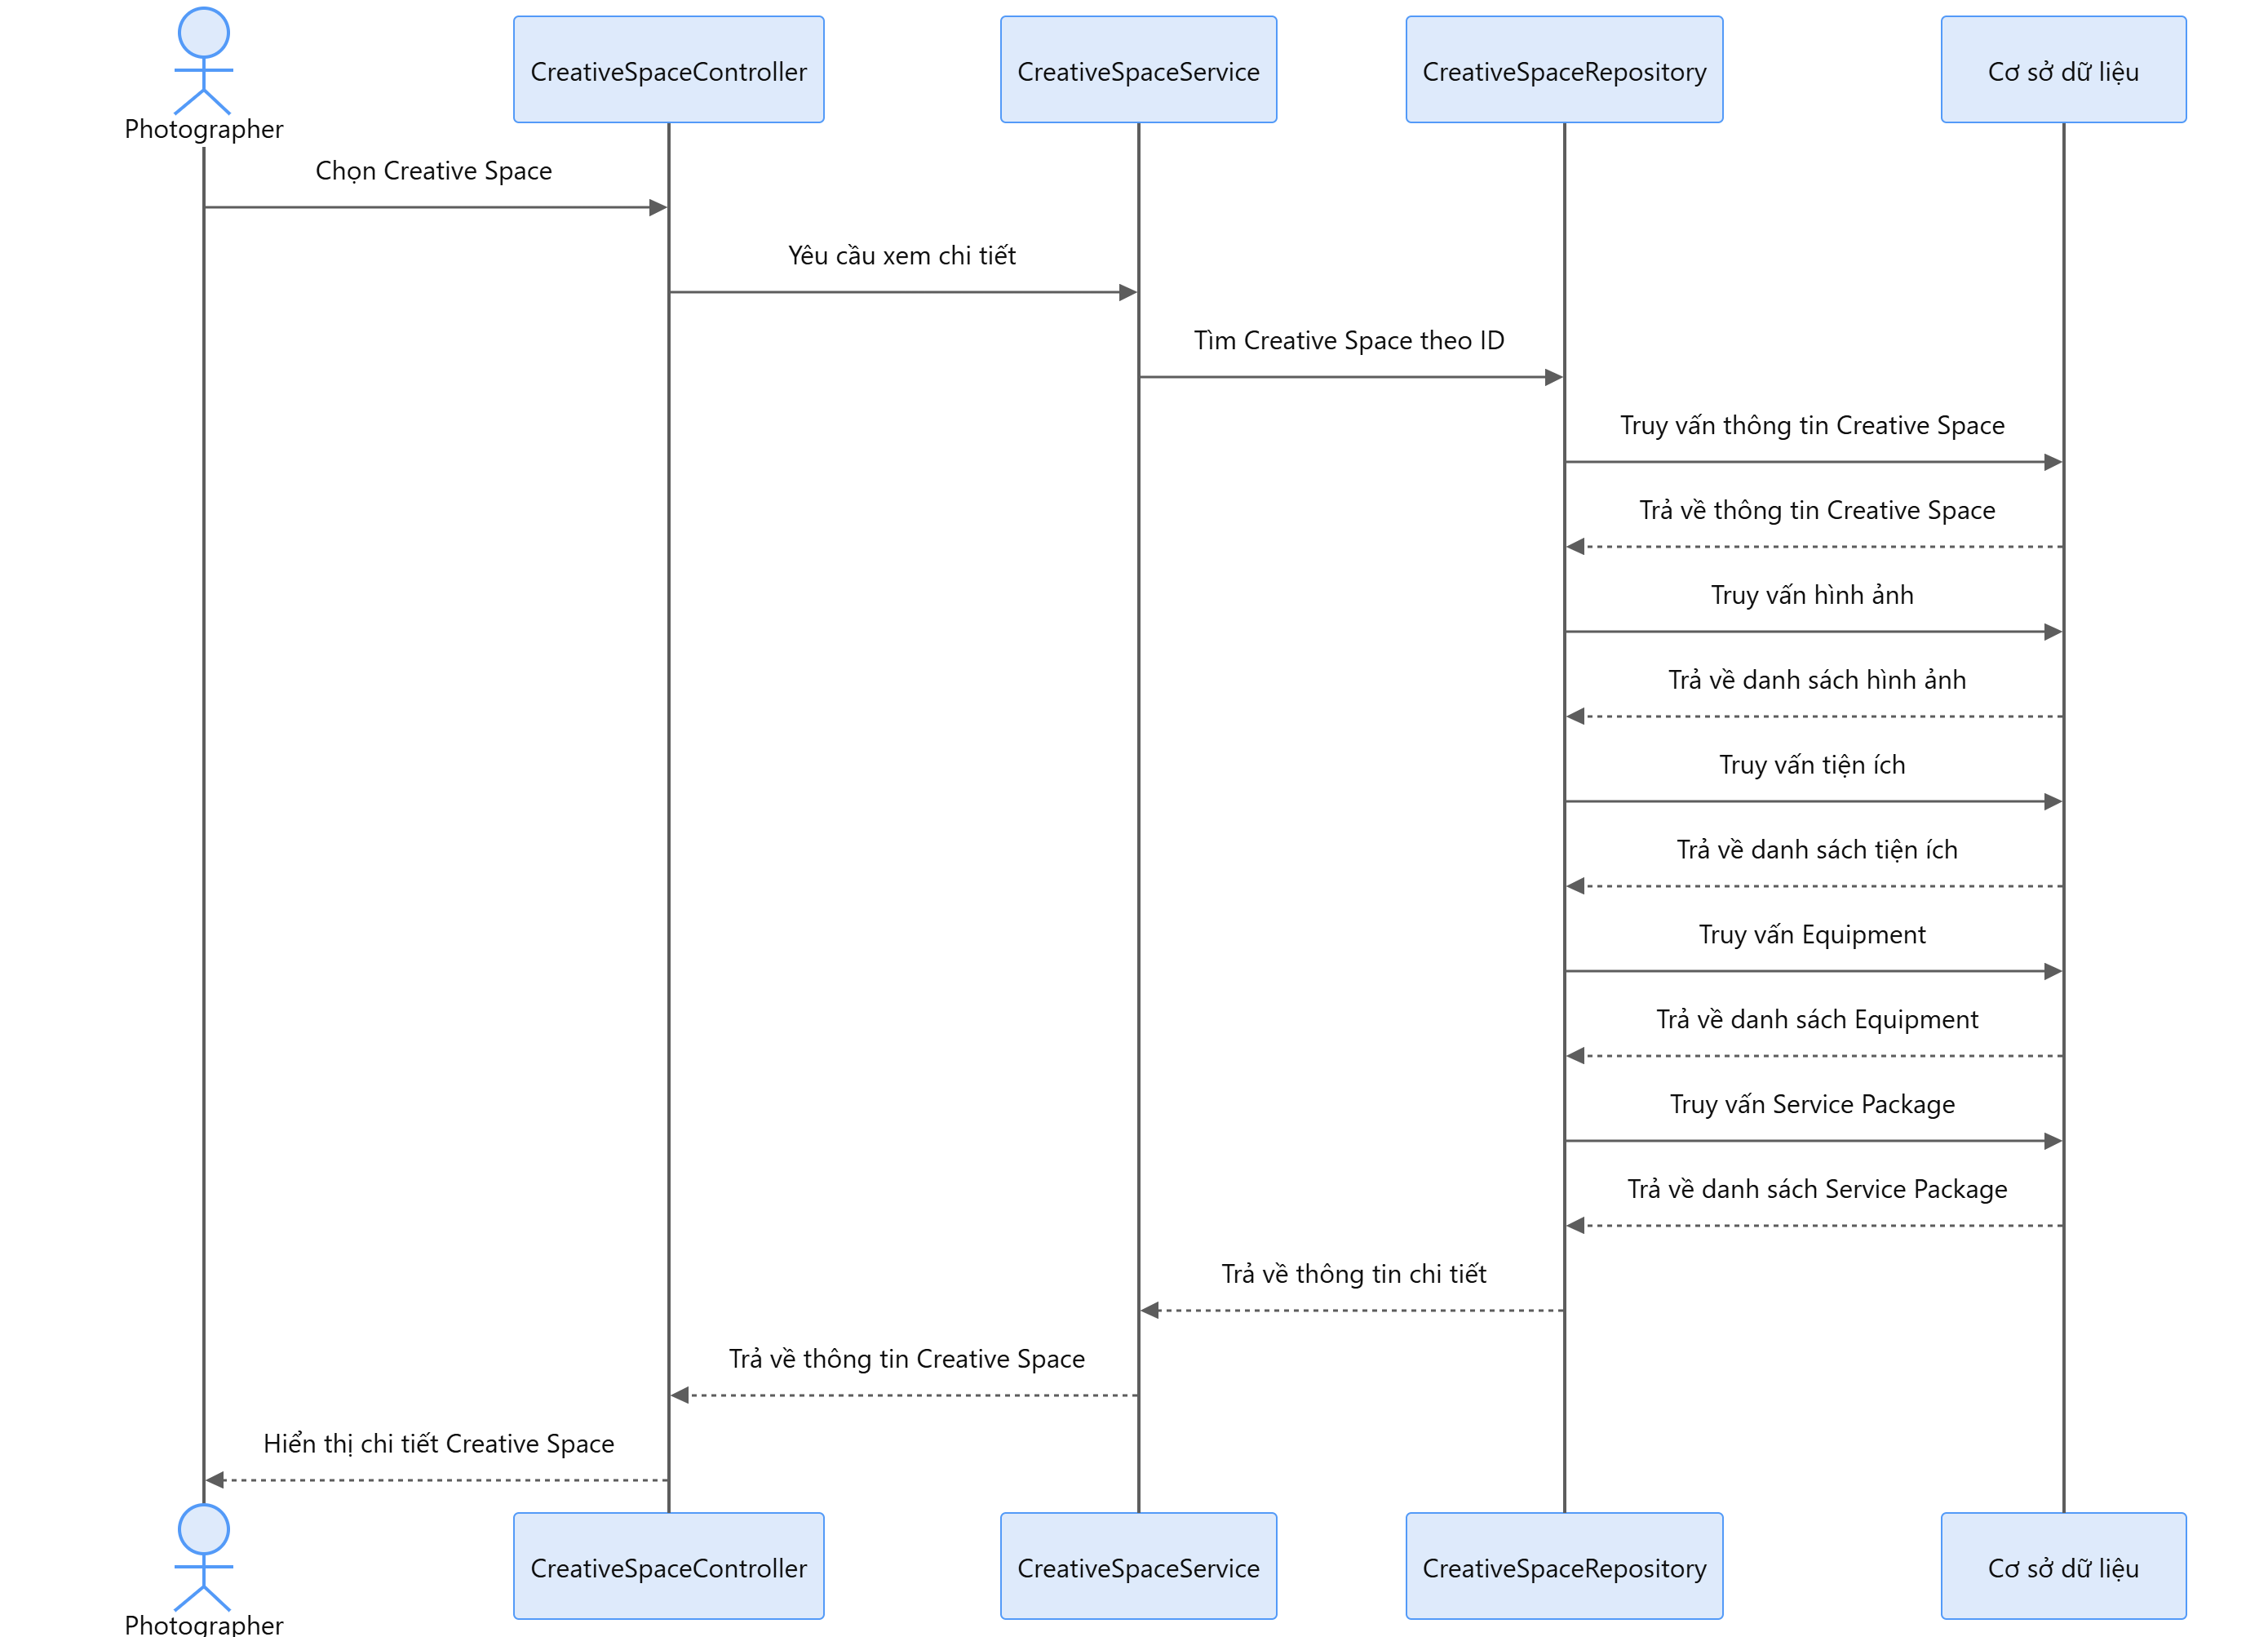
\includegraphics[width=1.1\textwidth]{images/25.png}
\end{figure}


% =========================================================
% 3.4 Reservation Management Module
% =========================================================

\subsection{Reservation Management Module}

\subsubsection{Đặt chỗ}

\paragraph{Class Diagram}

\begin{figure}[H]
	\centering
	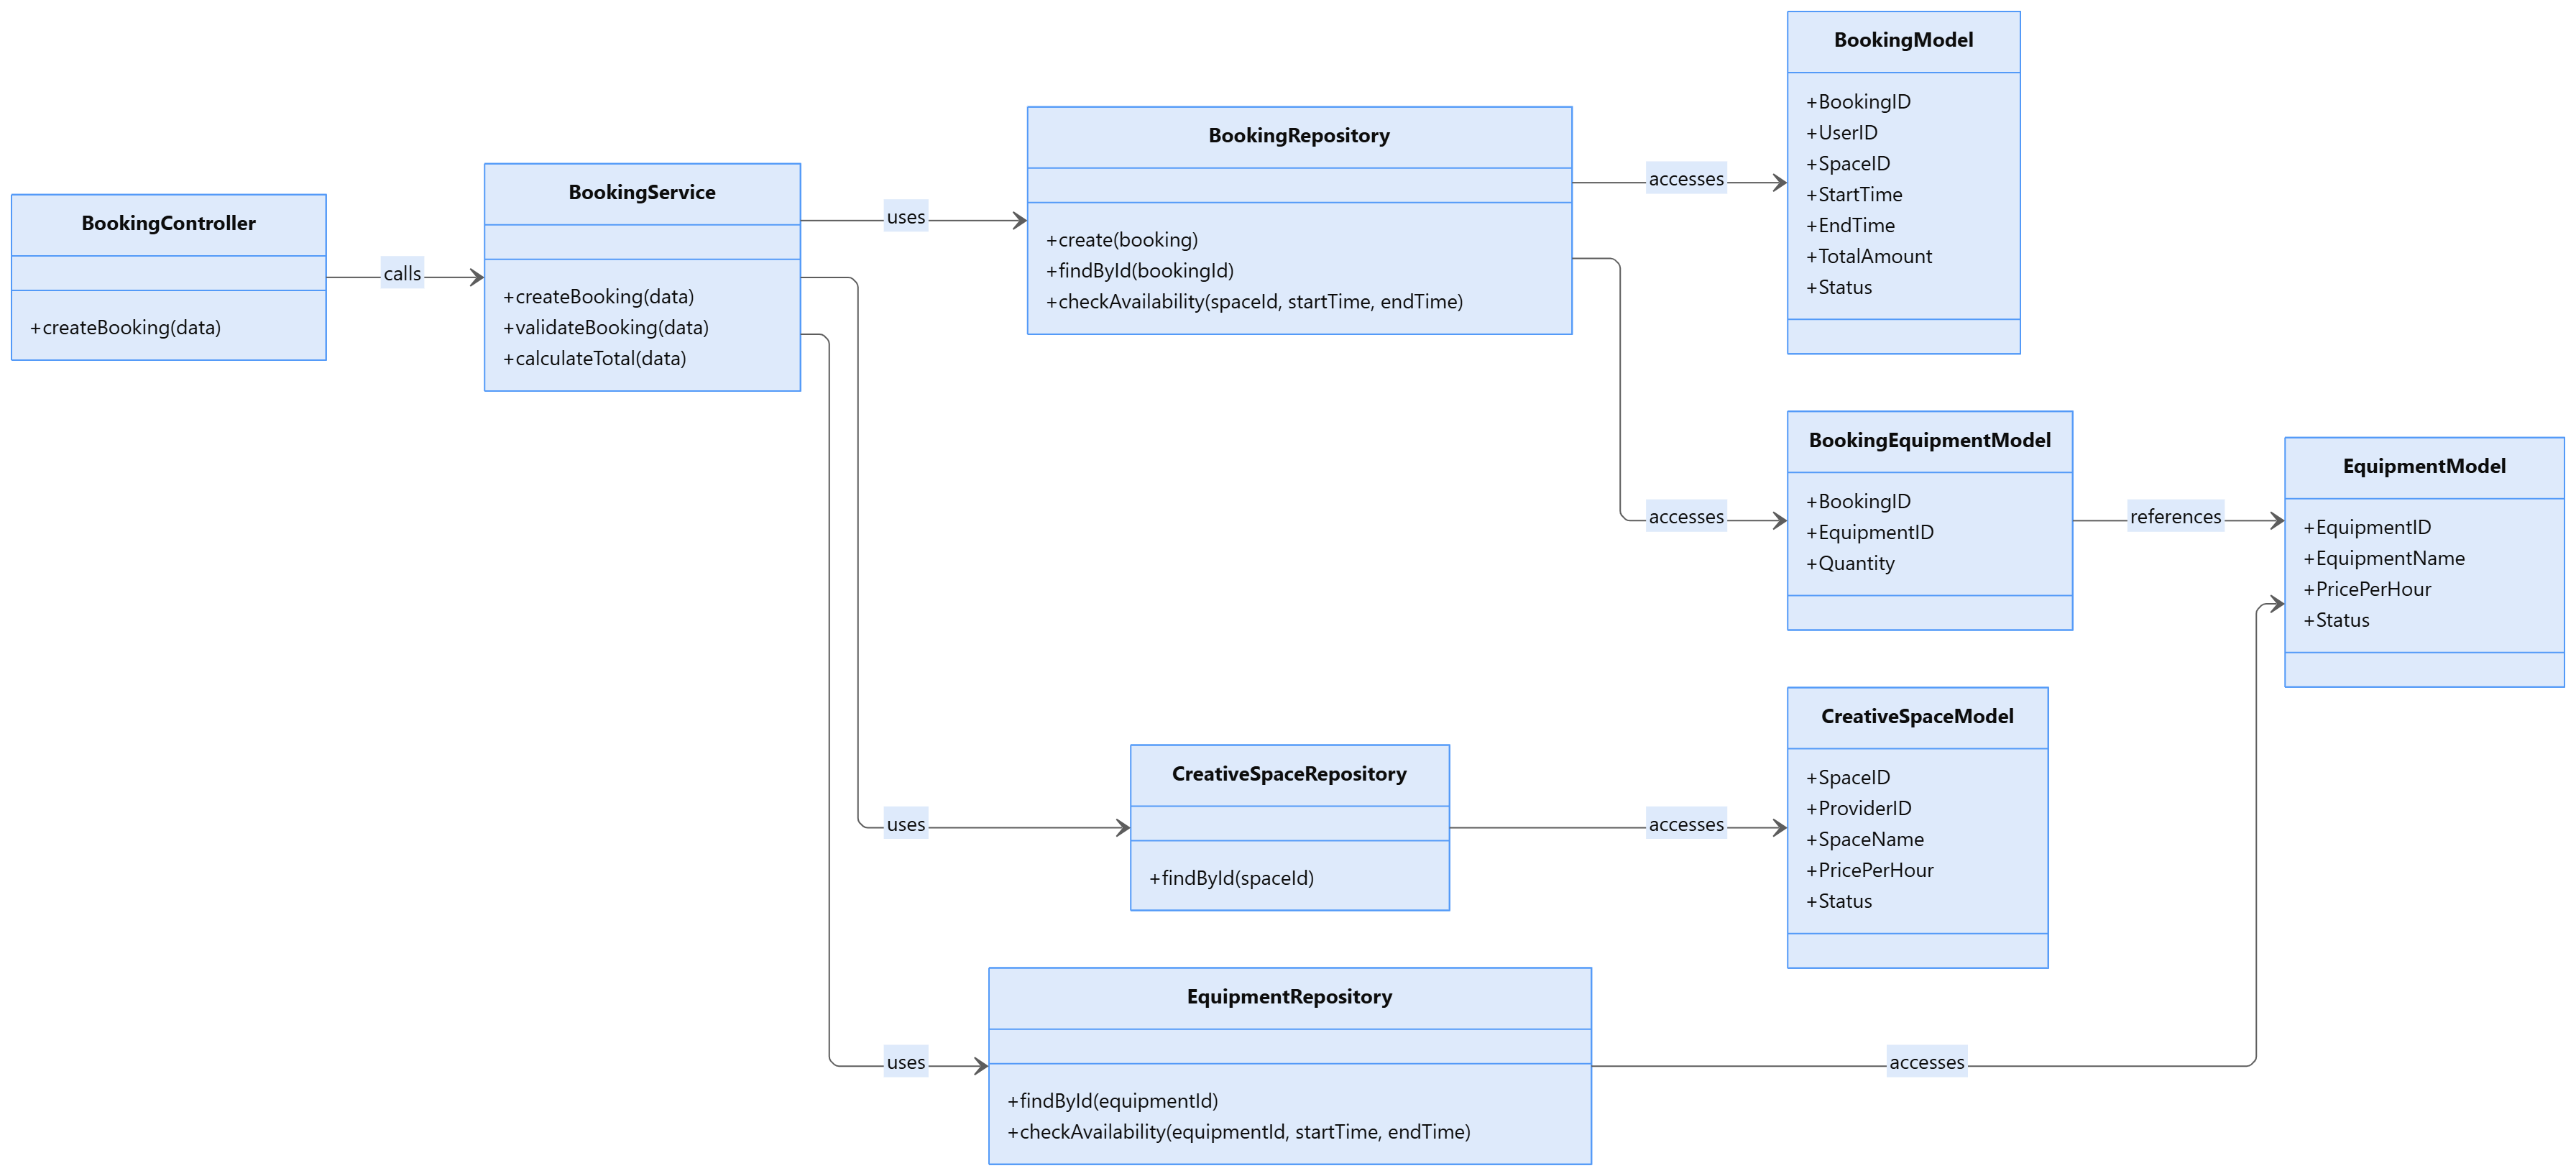
\includegraphics[width=1.1\textwidth]{images/26.png}
\end{figure}

\paragraph{Sequence Diagram}

\begin{figure}[H]
	\centering
	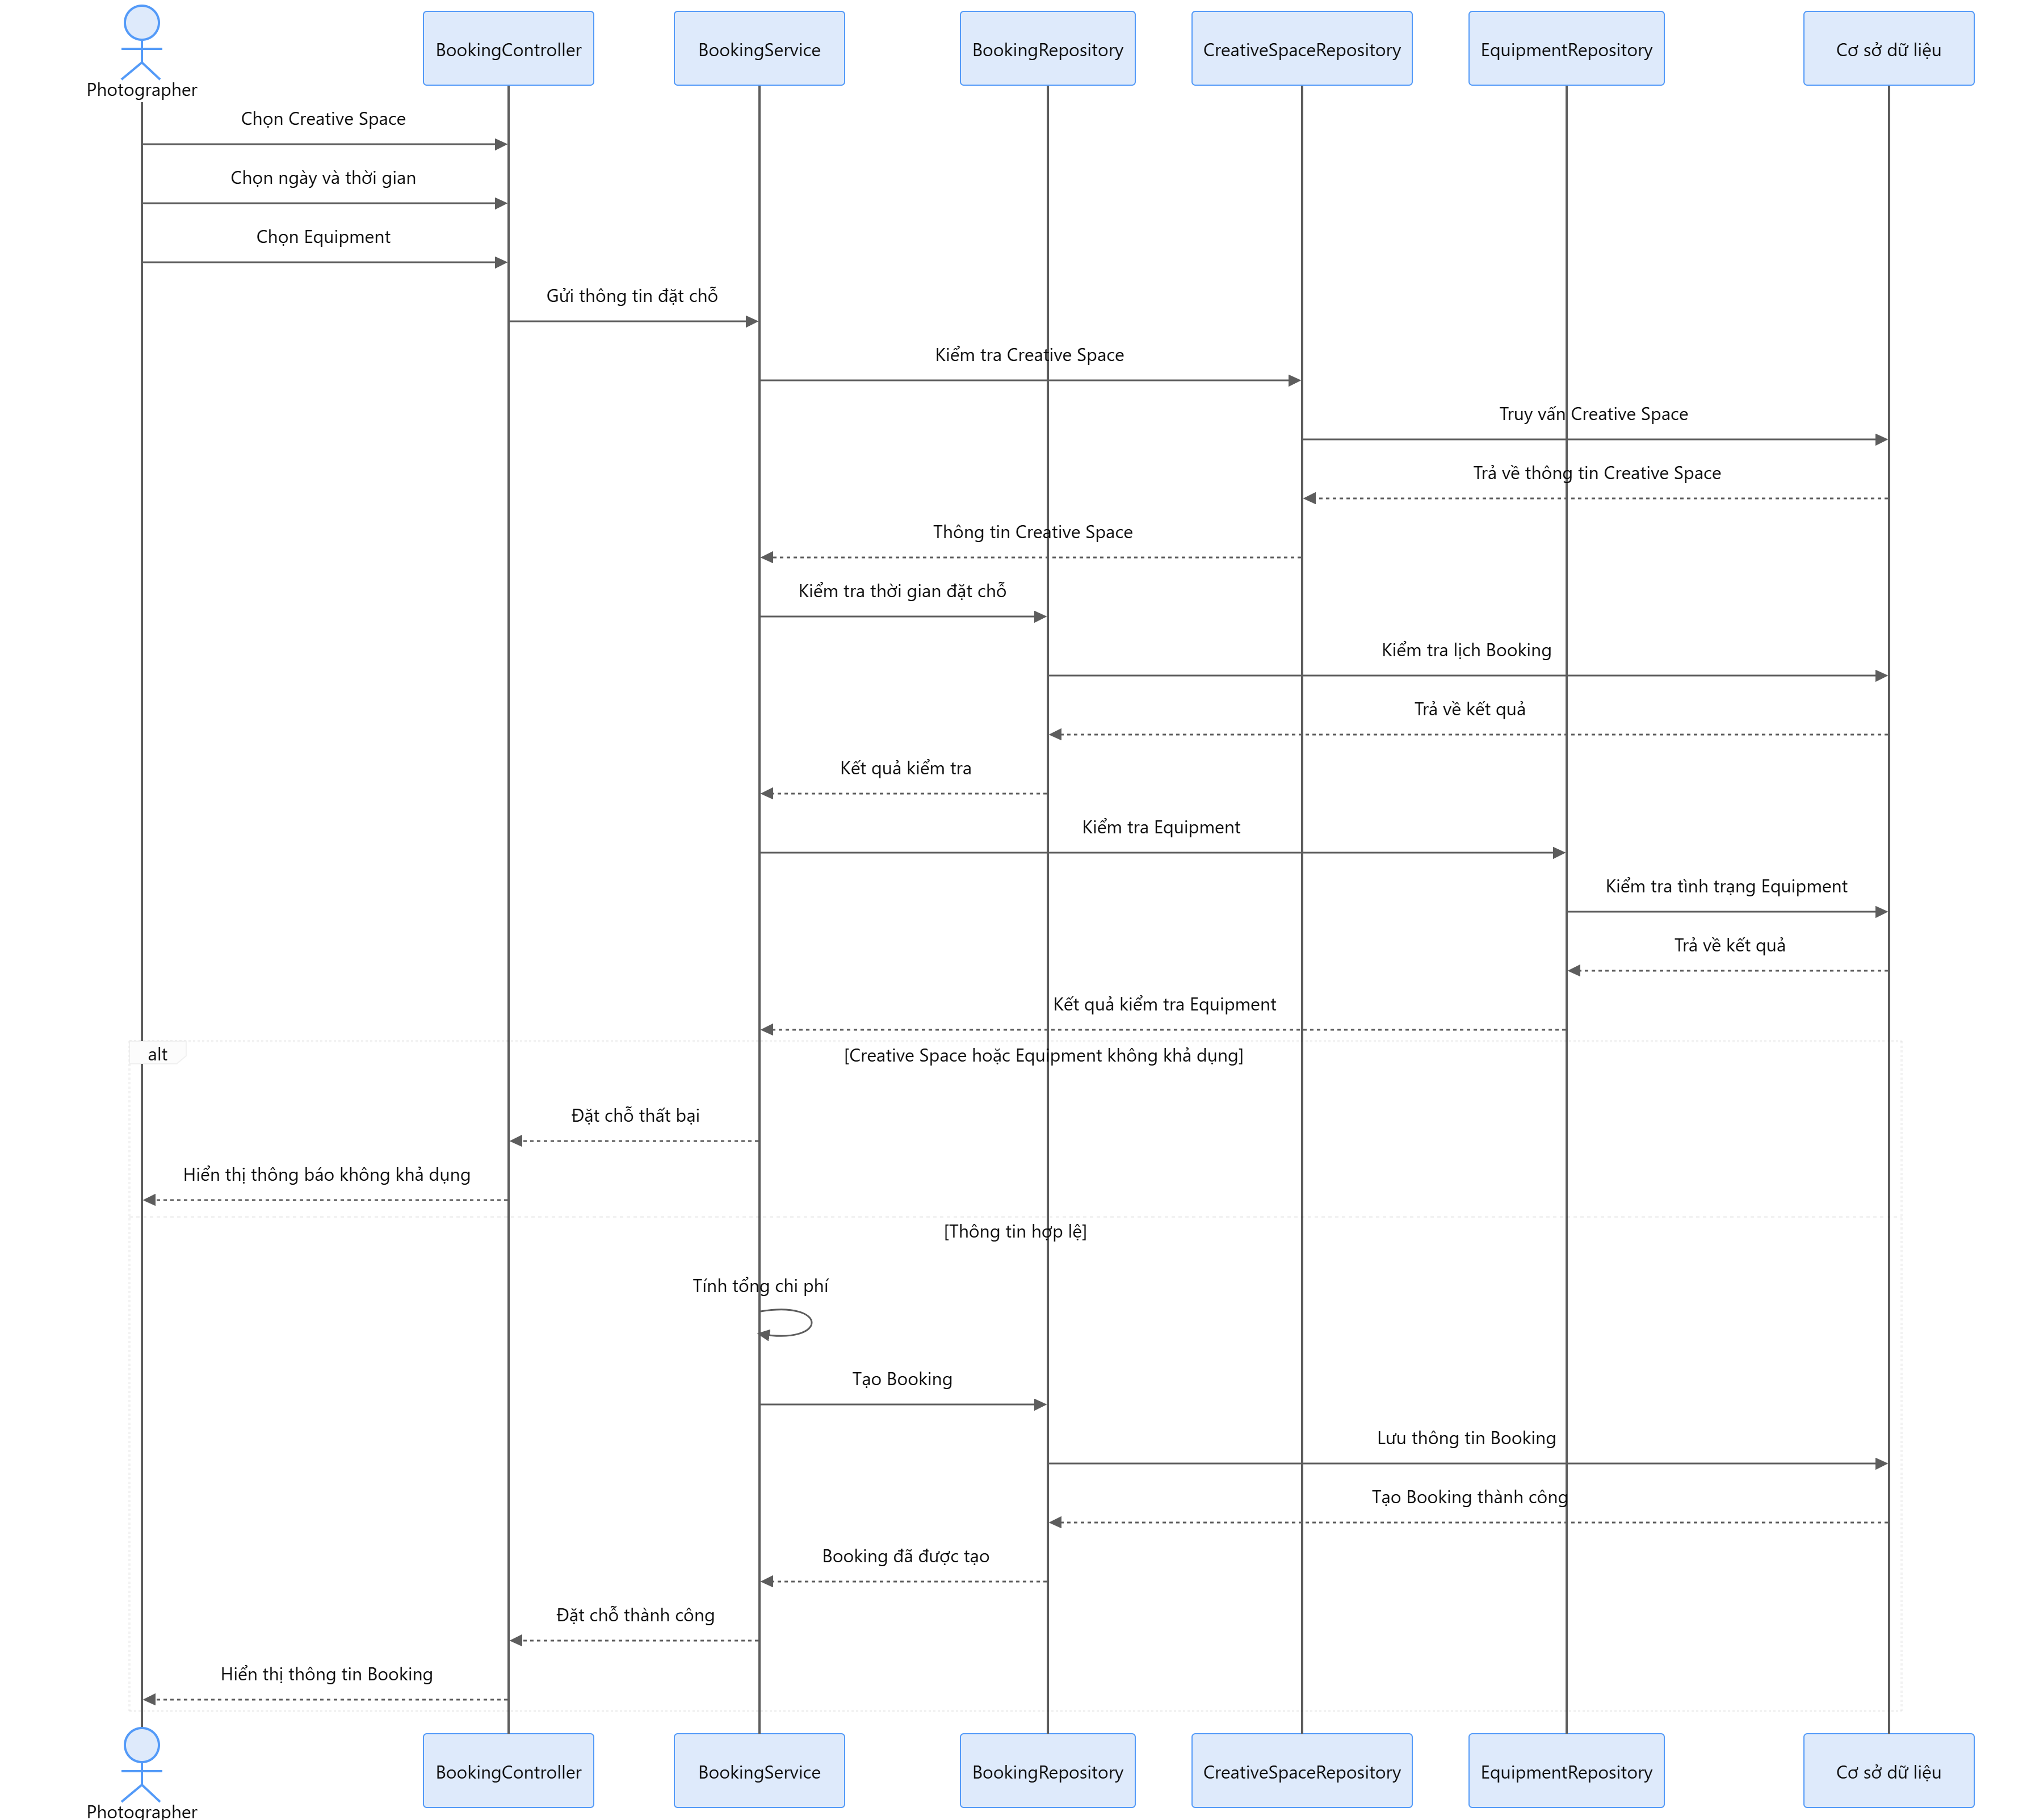
\includegraphics[width=1.1\textwidth]{images/27.png}
\end{figure}


\subsubsection{Hủy Booking}

\paragraph{Class Diagram}

\begin{figure}[H]
	\centering
	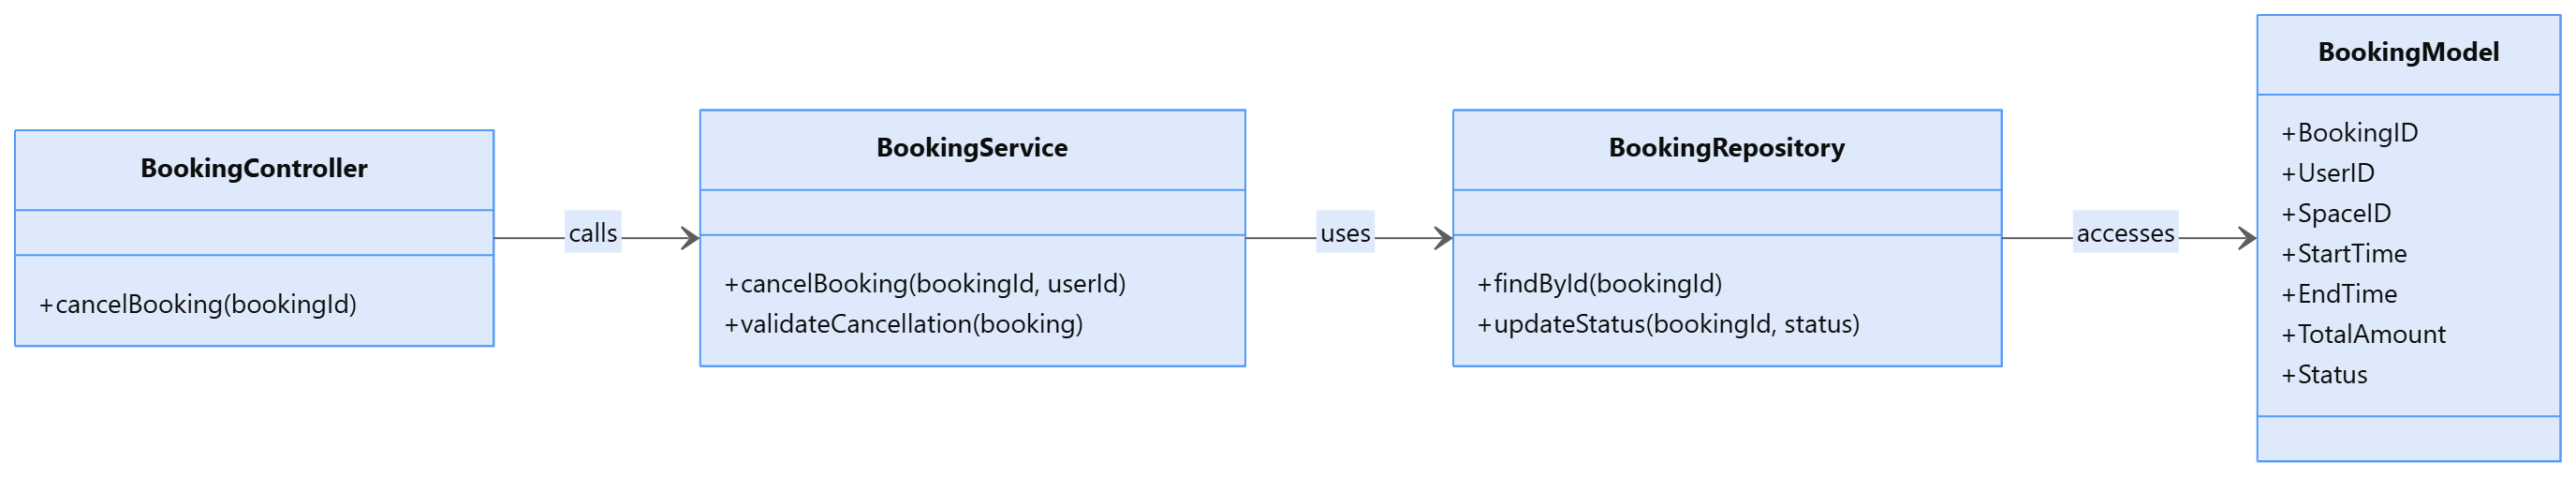
\includegraphics[width=1.1\textwidth]{images/28.png}
\end{figure}

\paragraph{Sequence Diagram}

\begin{figure}[H]
	\centering
	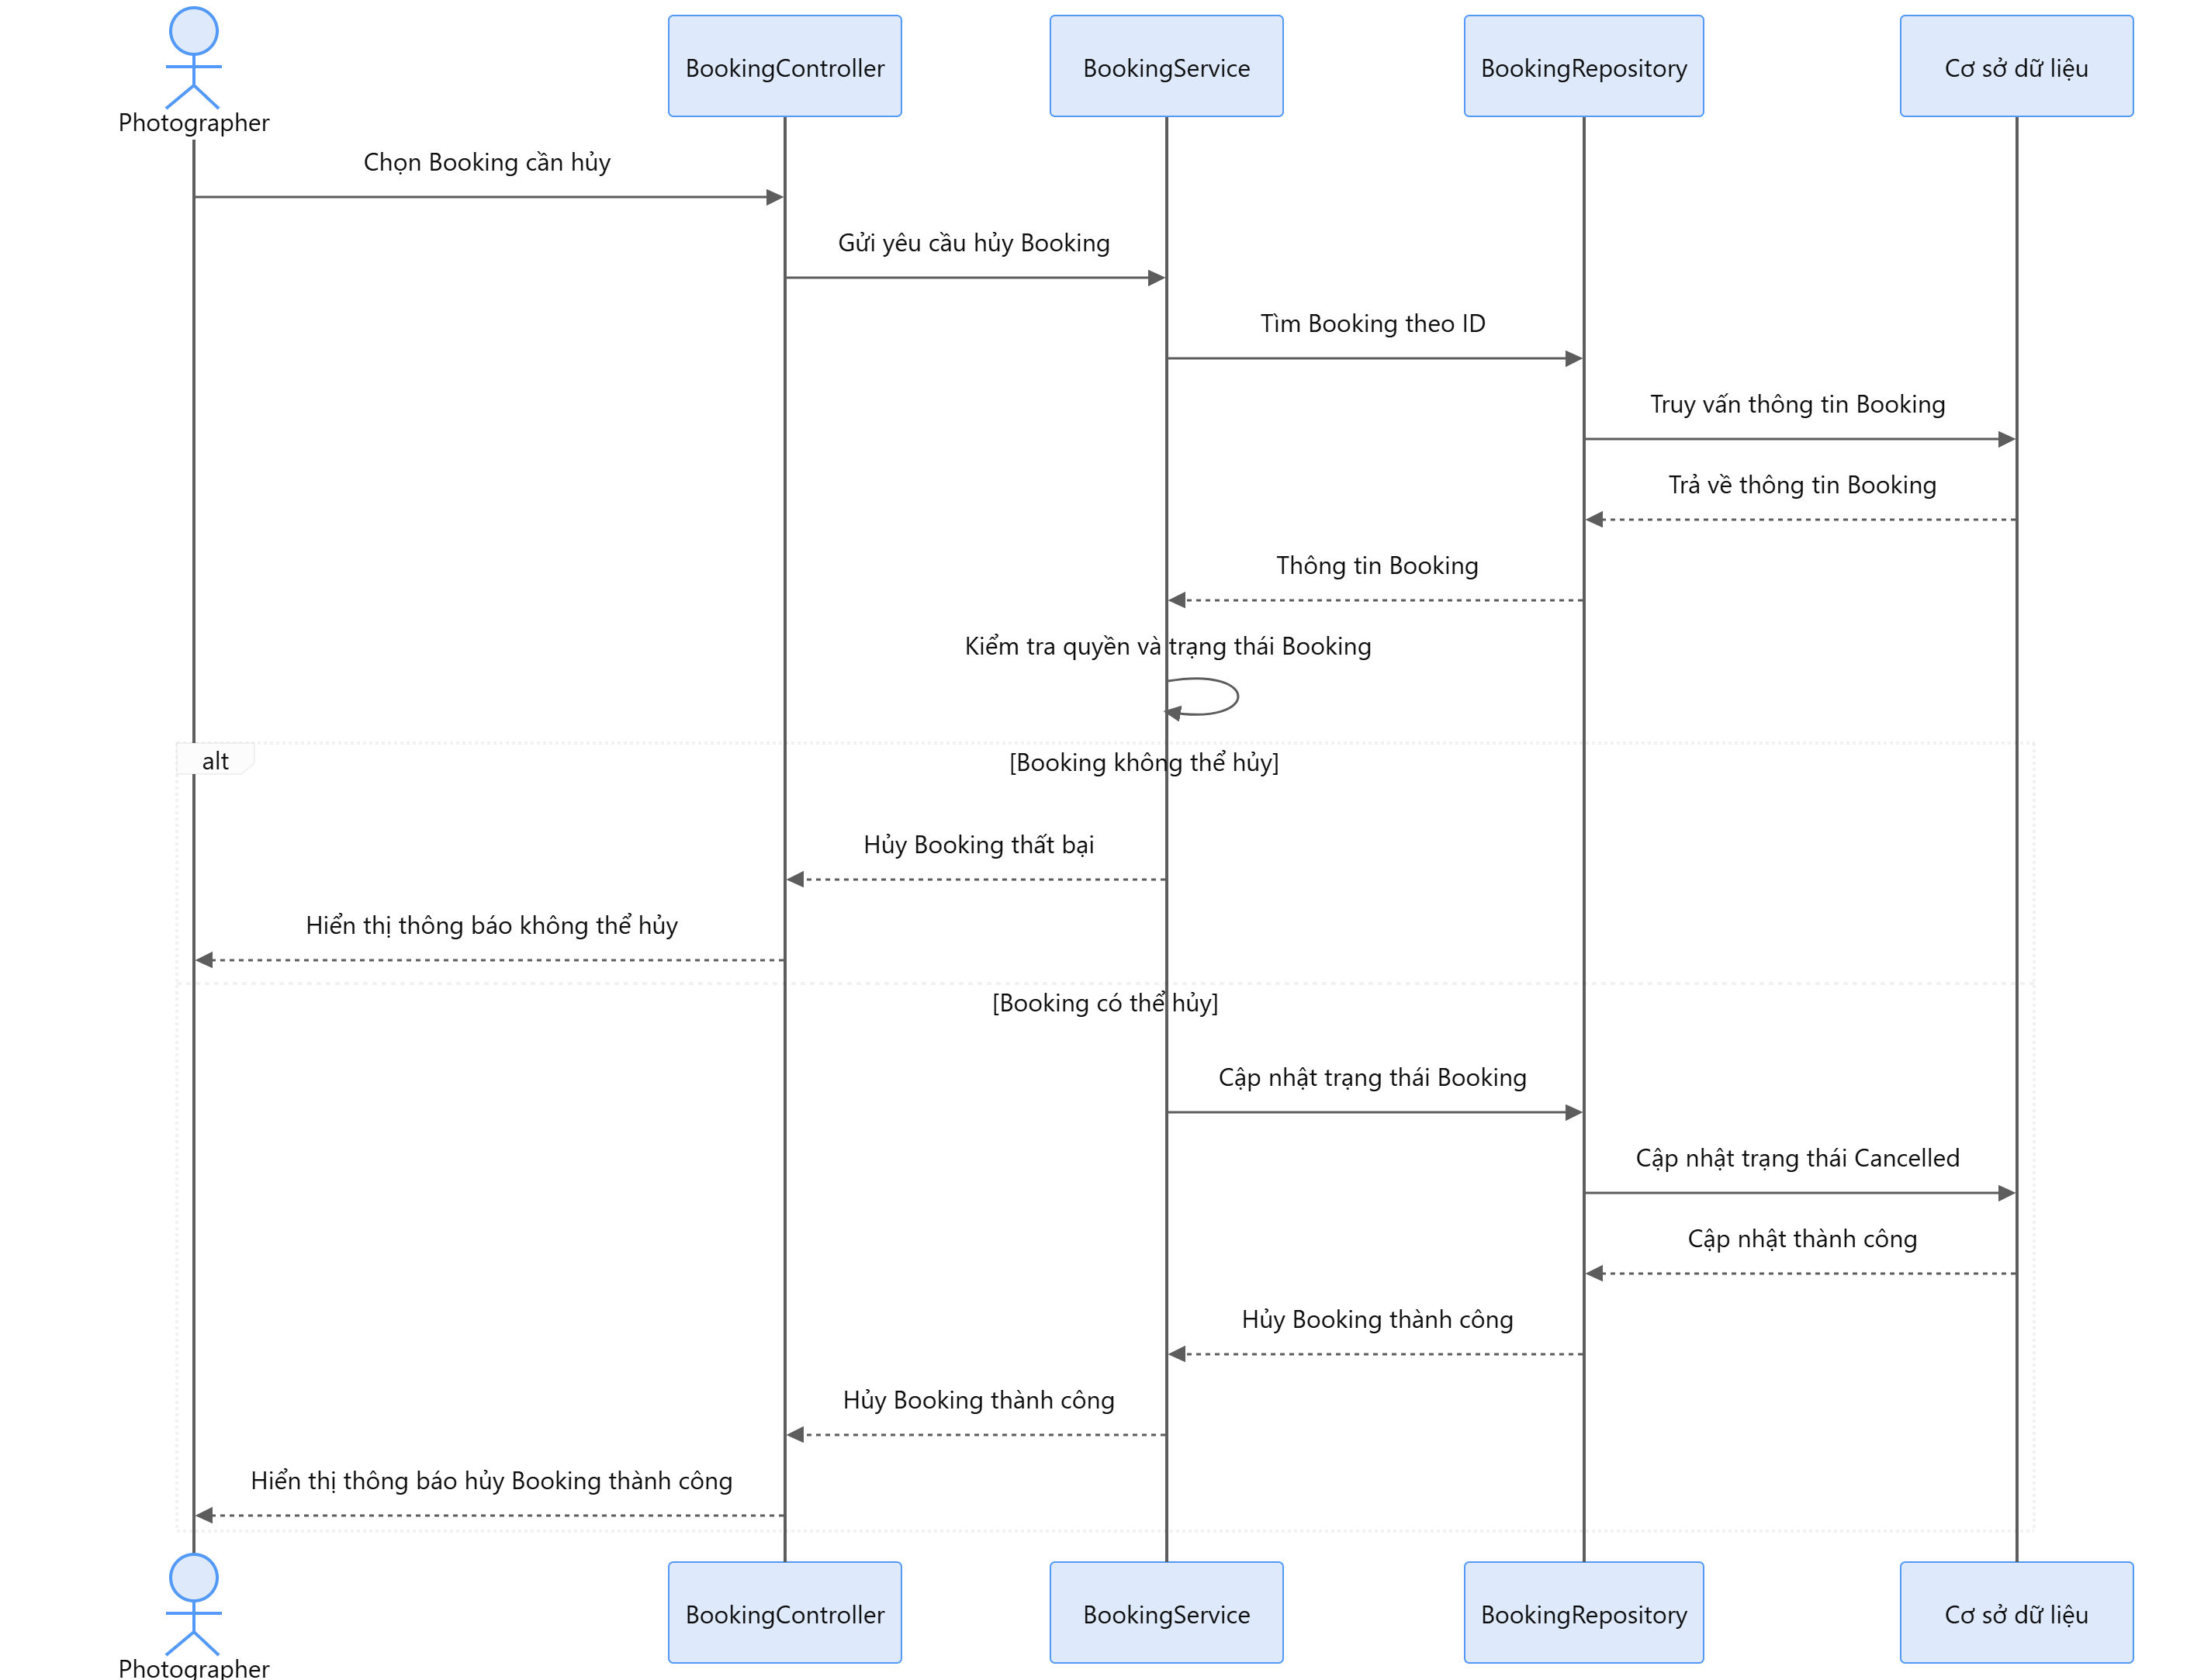
\includegraphics[width=1.1\textwidth]{images/29.png}
\end{figure}


% =========================================================
% 3.5 Payment and Booking Management Module
% =========================================================

\subsection{Payment and Booking Management Module}

\subsubsection{Thanh toán}

\paragraph{Class Diagram}

\begin{figure}[H]
	\centering
	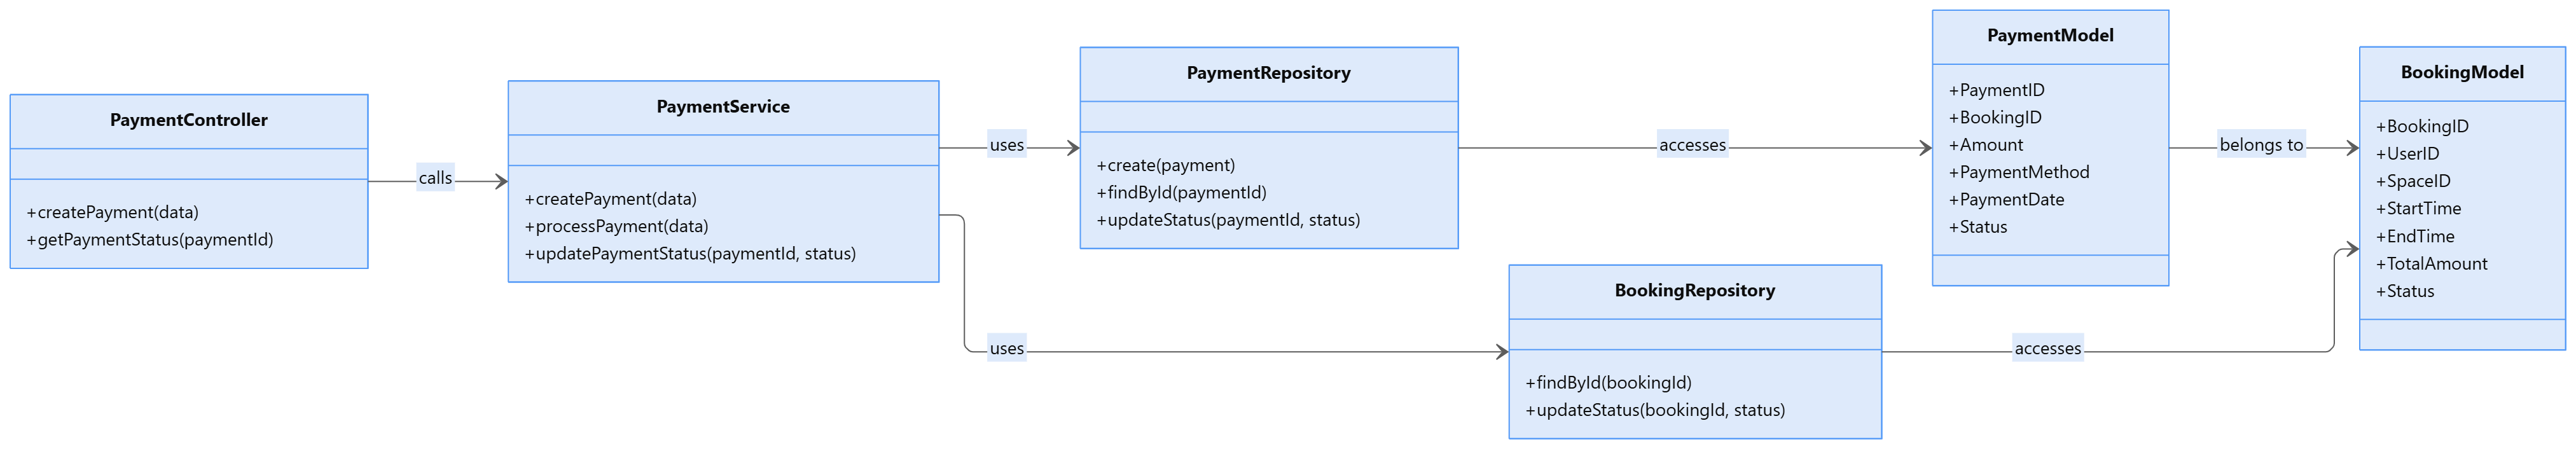
\includegraphics[width=1.1\textwidth]{images/30.png}
\end{figure}

\paragraph{Sequence Diagram}

\begin{figure}[H]
	\centering
	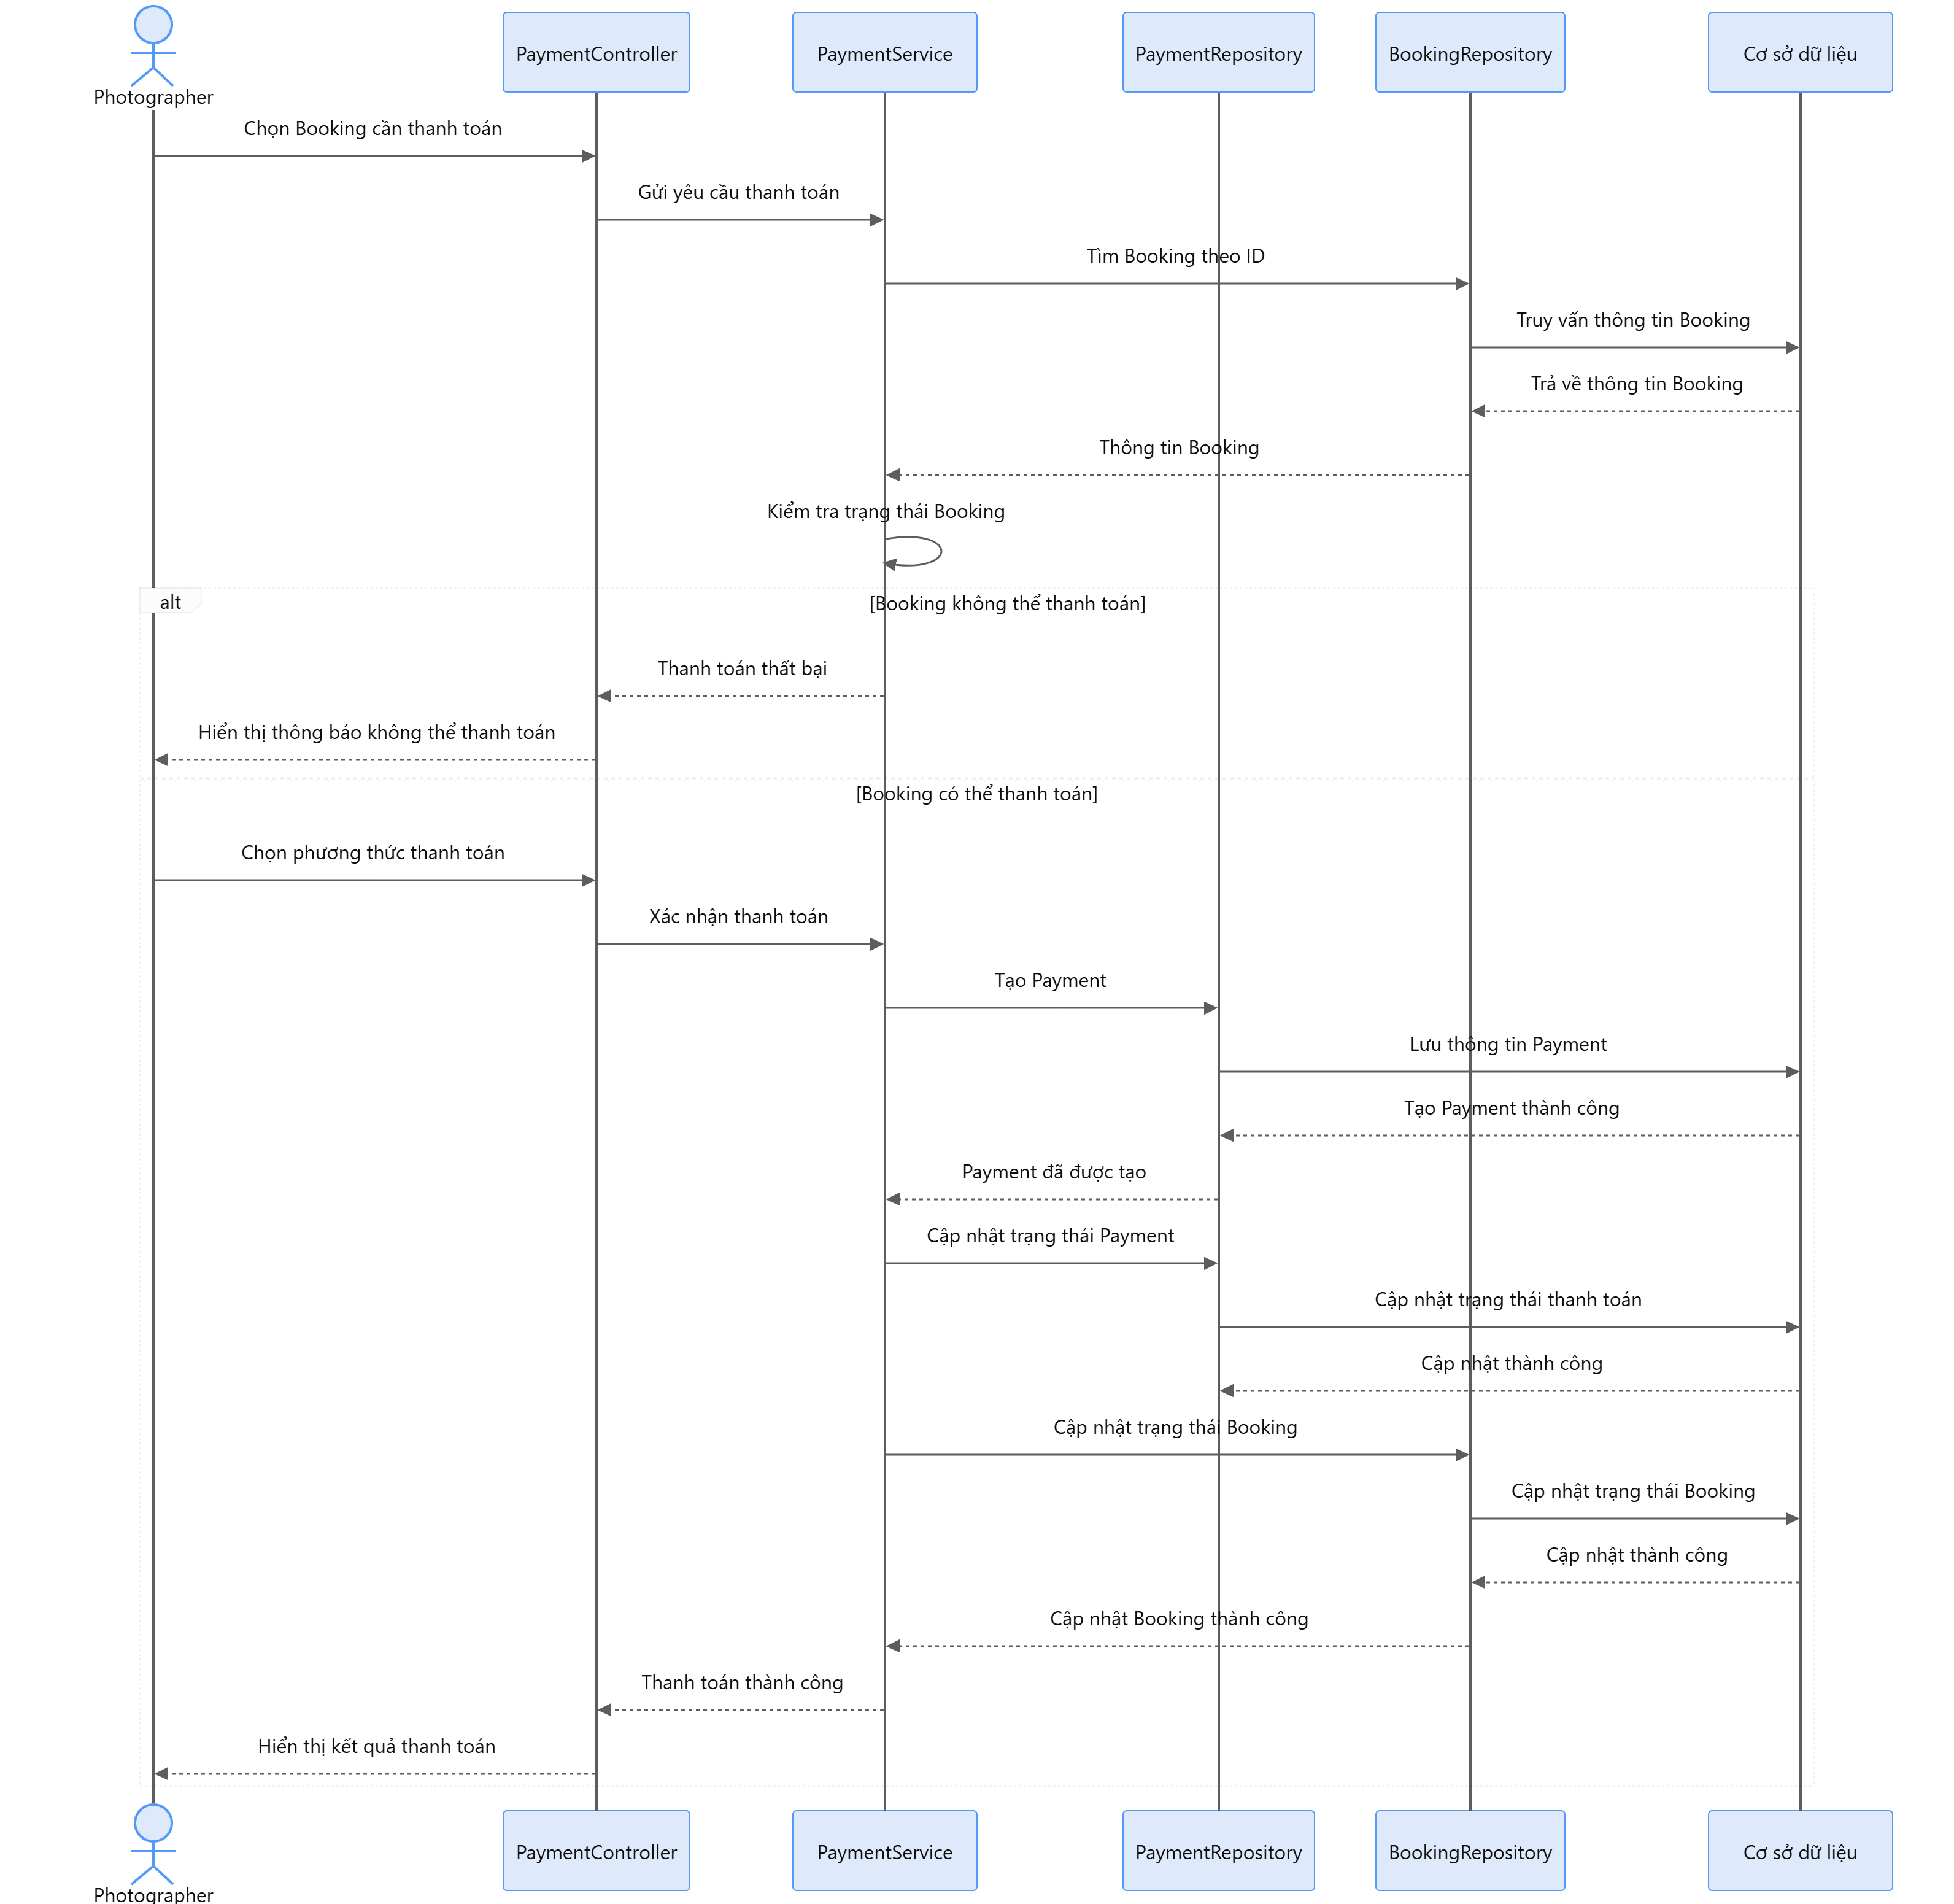
\includegraphics[width=1.1\textwidth]{images/31.png}
\end{figure}


% =========================================================
% 3.6 Workshop Management Module
% =========================================================

\subsection{Workshop Management Module}

\subsubsection{Đăng ký Workshop}

\paragraph{Class Diagram}

\begin{figure}[H]
	\centering
	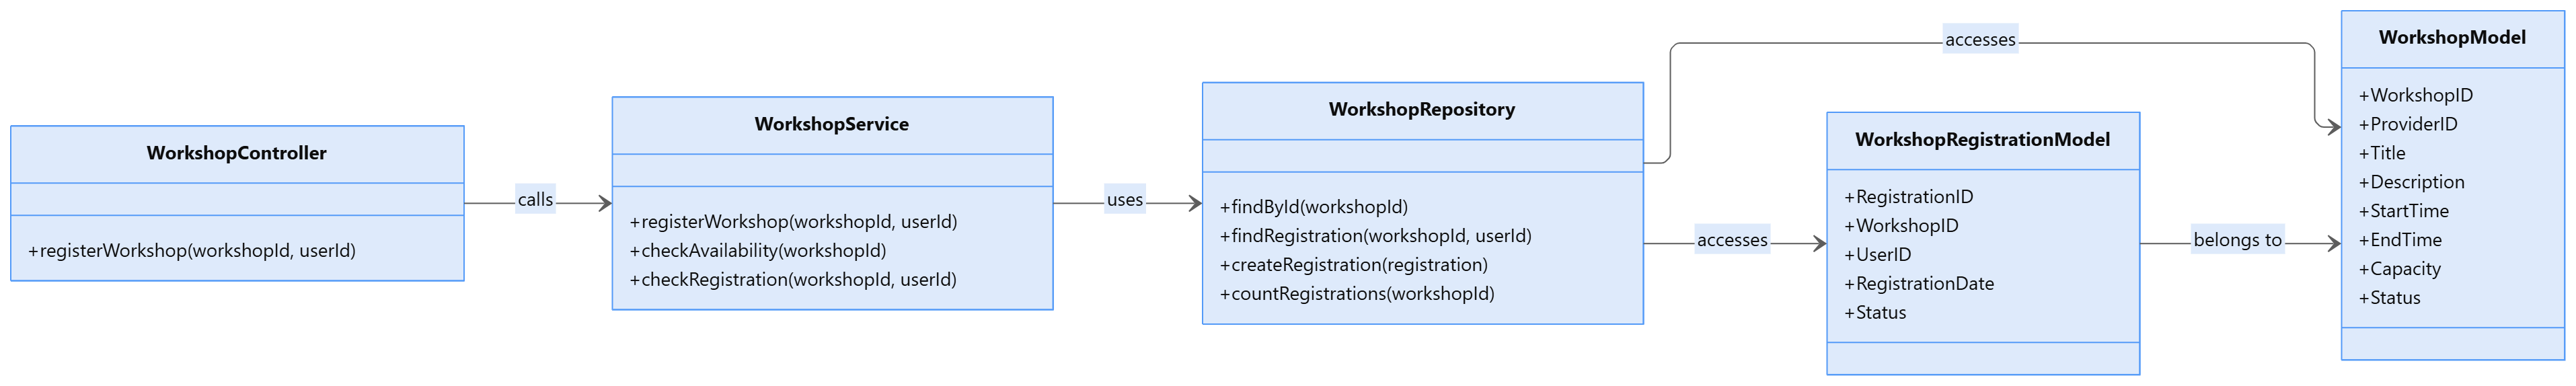
\includegraphics[width=1.1\textwidth]{images/32.png}
\end{figure}

\paragraph{Sequence Diagram}

\begin{figure}[H]
	\centering
	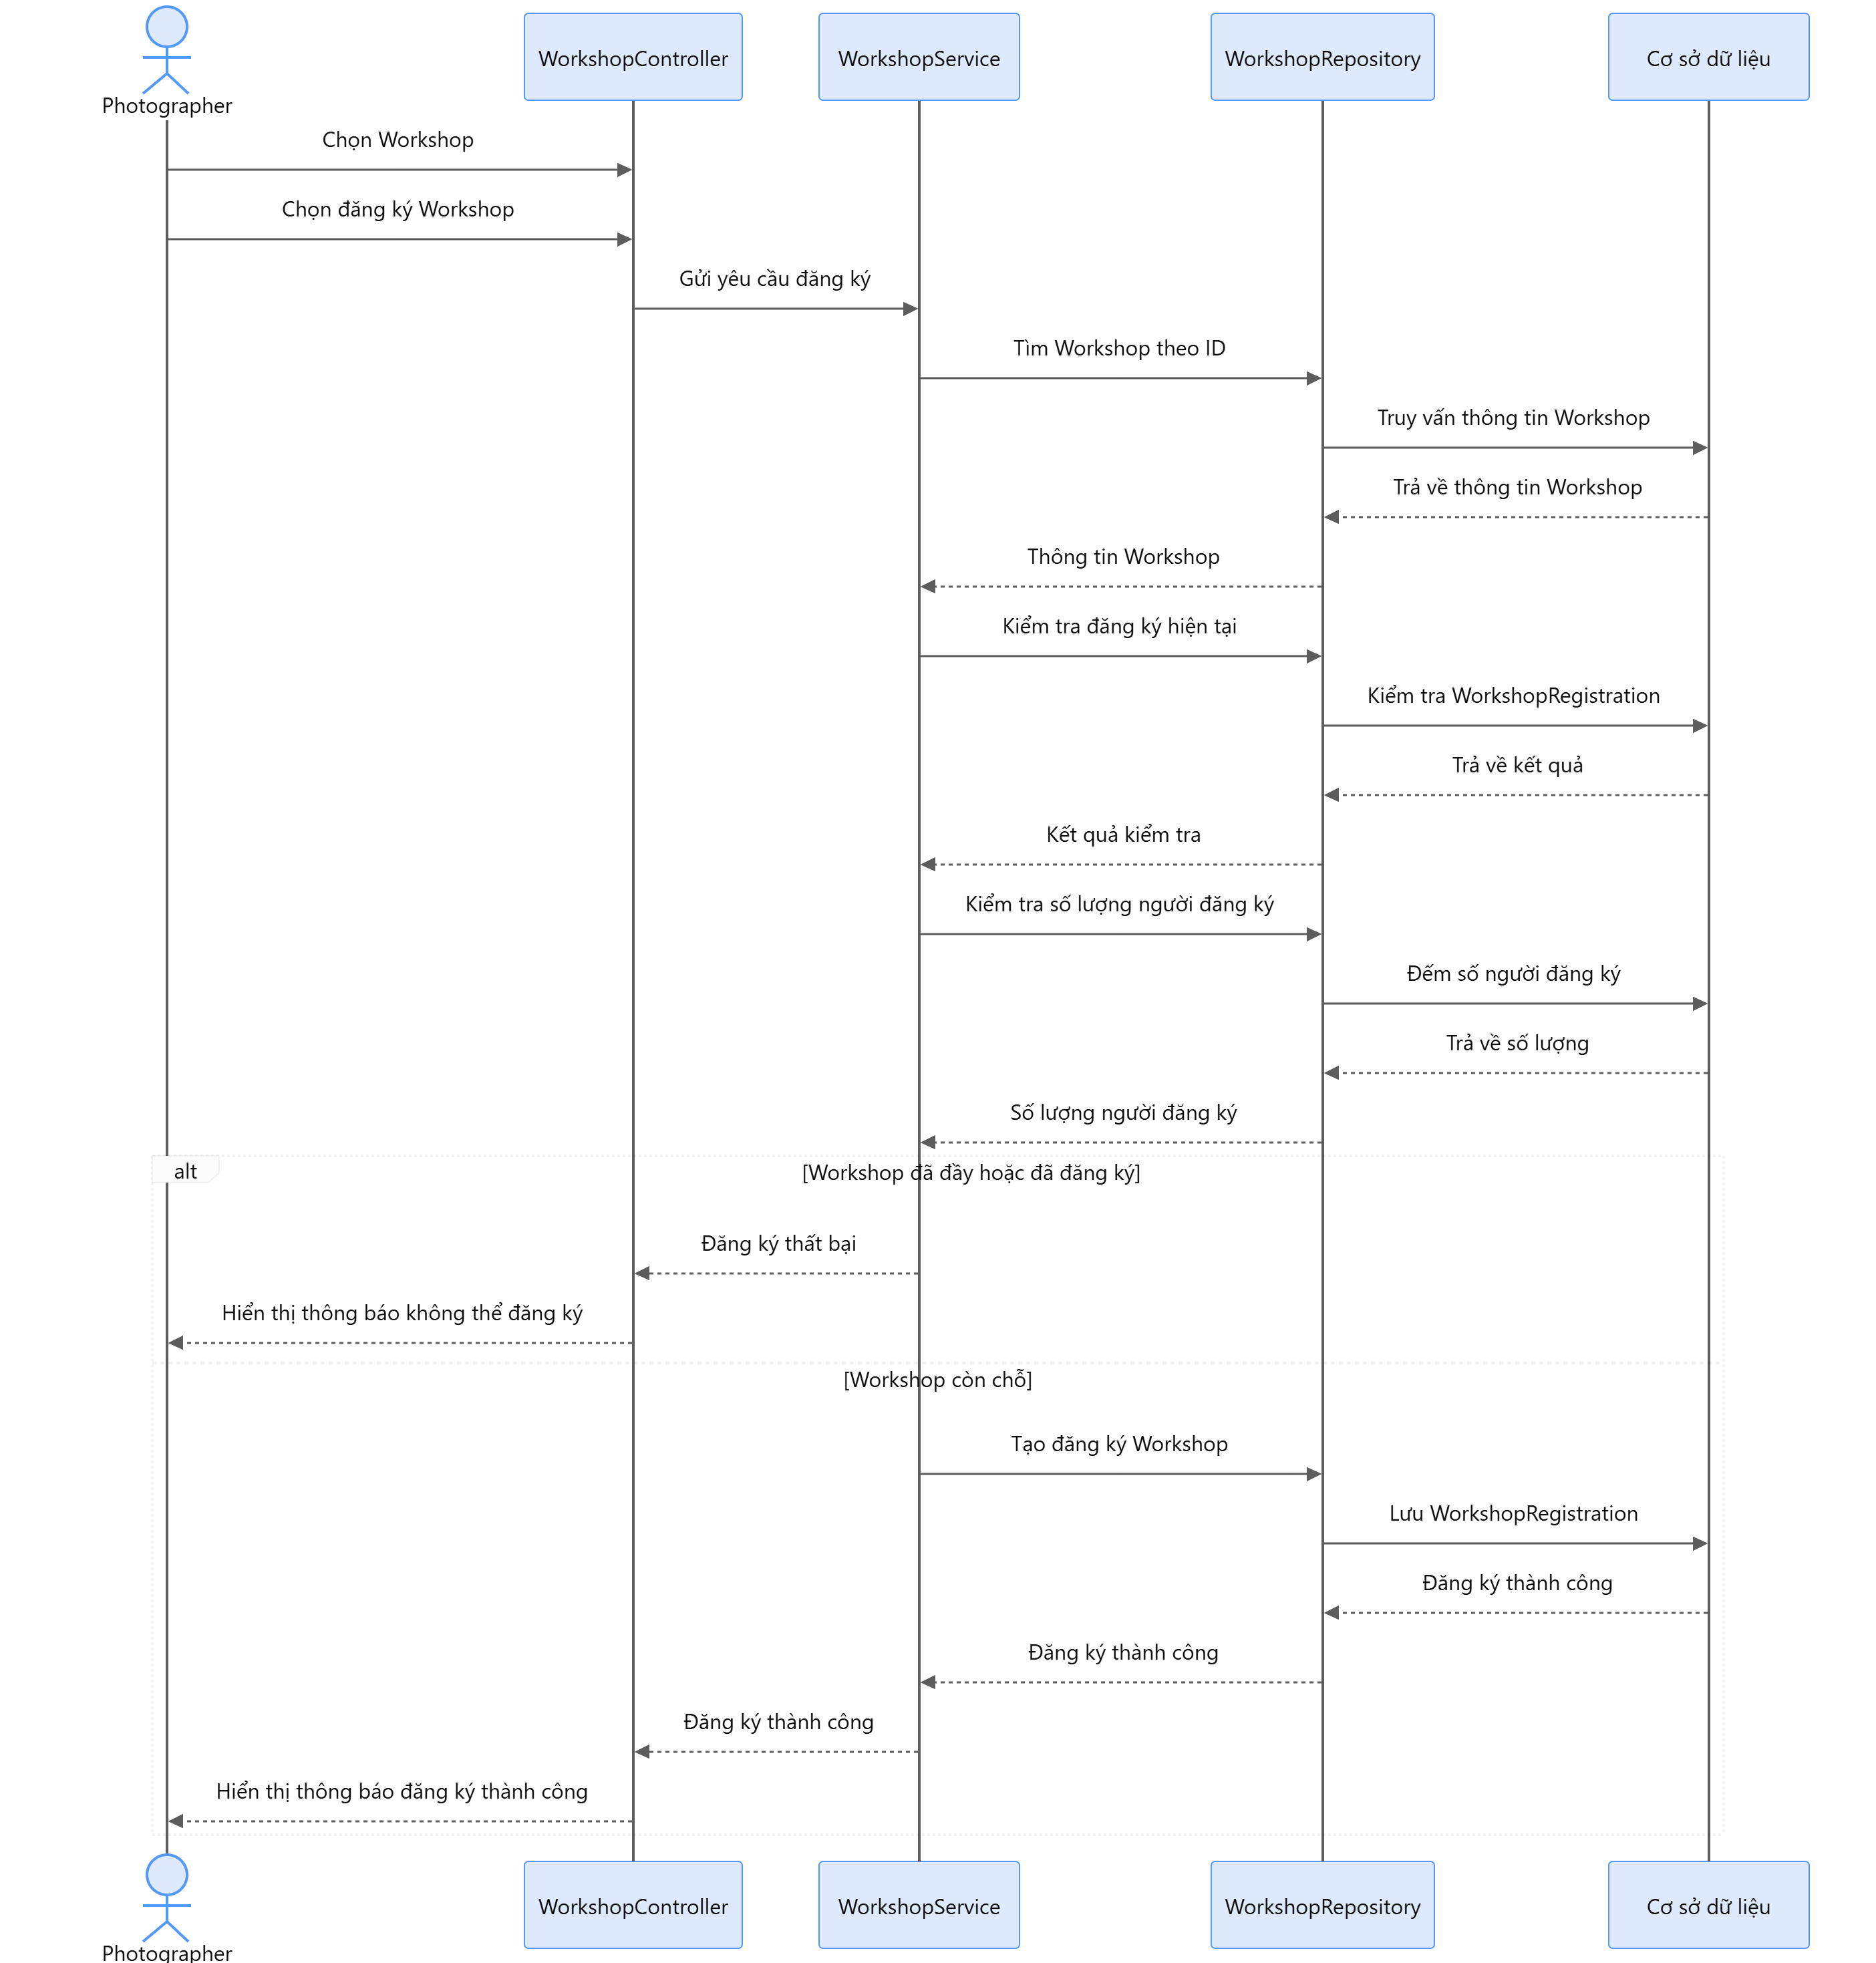
\includegraphics[width=1.1\textwidth]{images/33.png}
\end{figure}


% =========================================================
% 3.7 Service Provider Management Module
% =========================================================

\subsection{Service Provider Management Module}

\subsubsection{Quản lý hồ sơ Provider}

\paragraph{Class Diagram}

\begin{figure}[H]
	\centering
	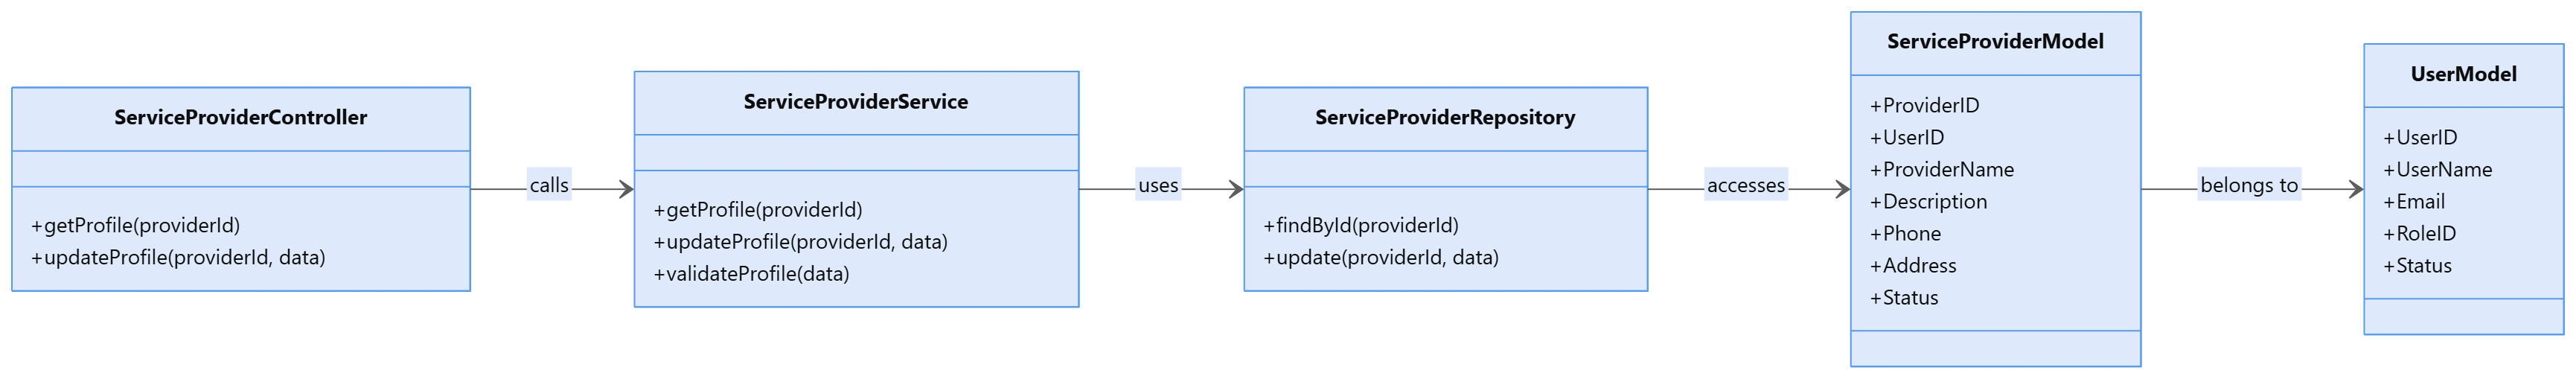
\includegraphics[width=1.1\textwidth]{images/34.png}
\end{figure}

\paragraph{Sequence Diagram}

\begin{figure}[H]
	\centering
	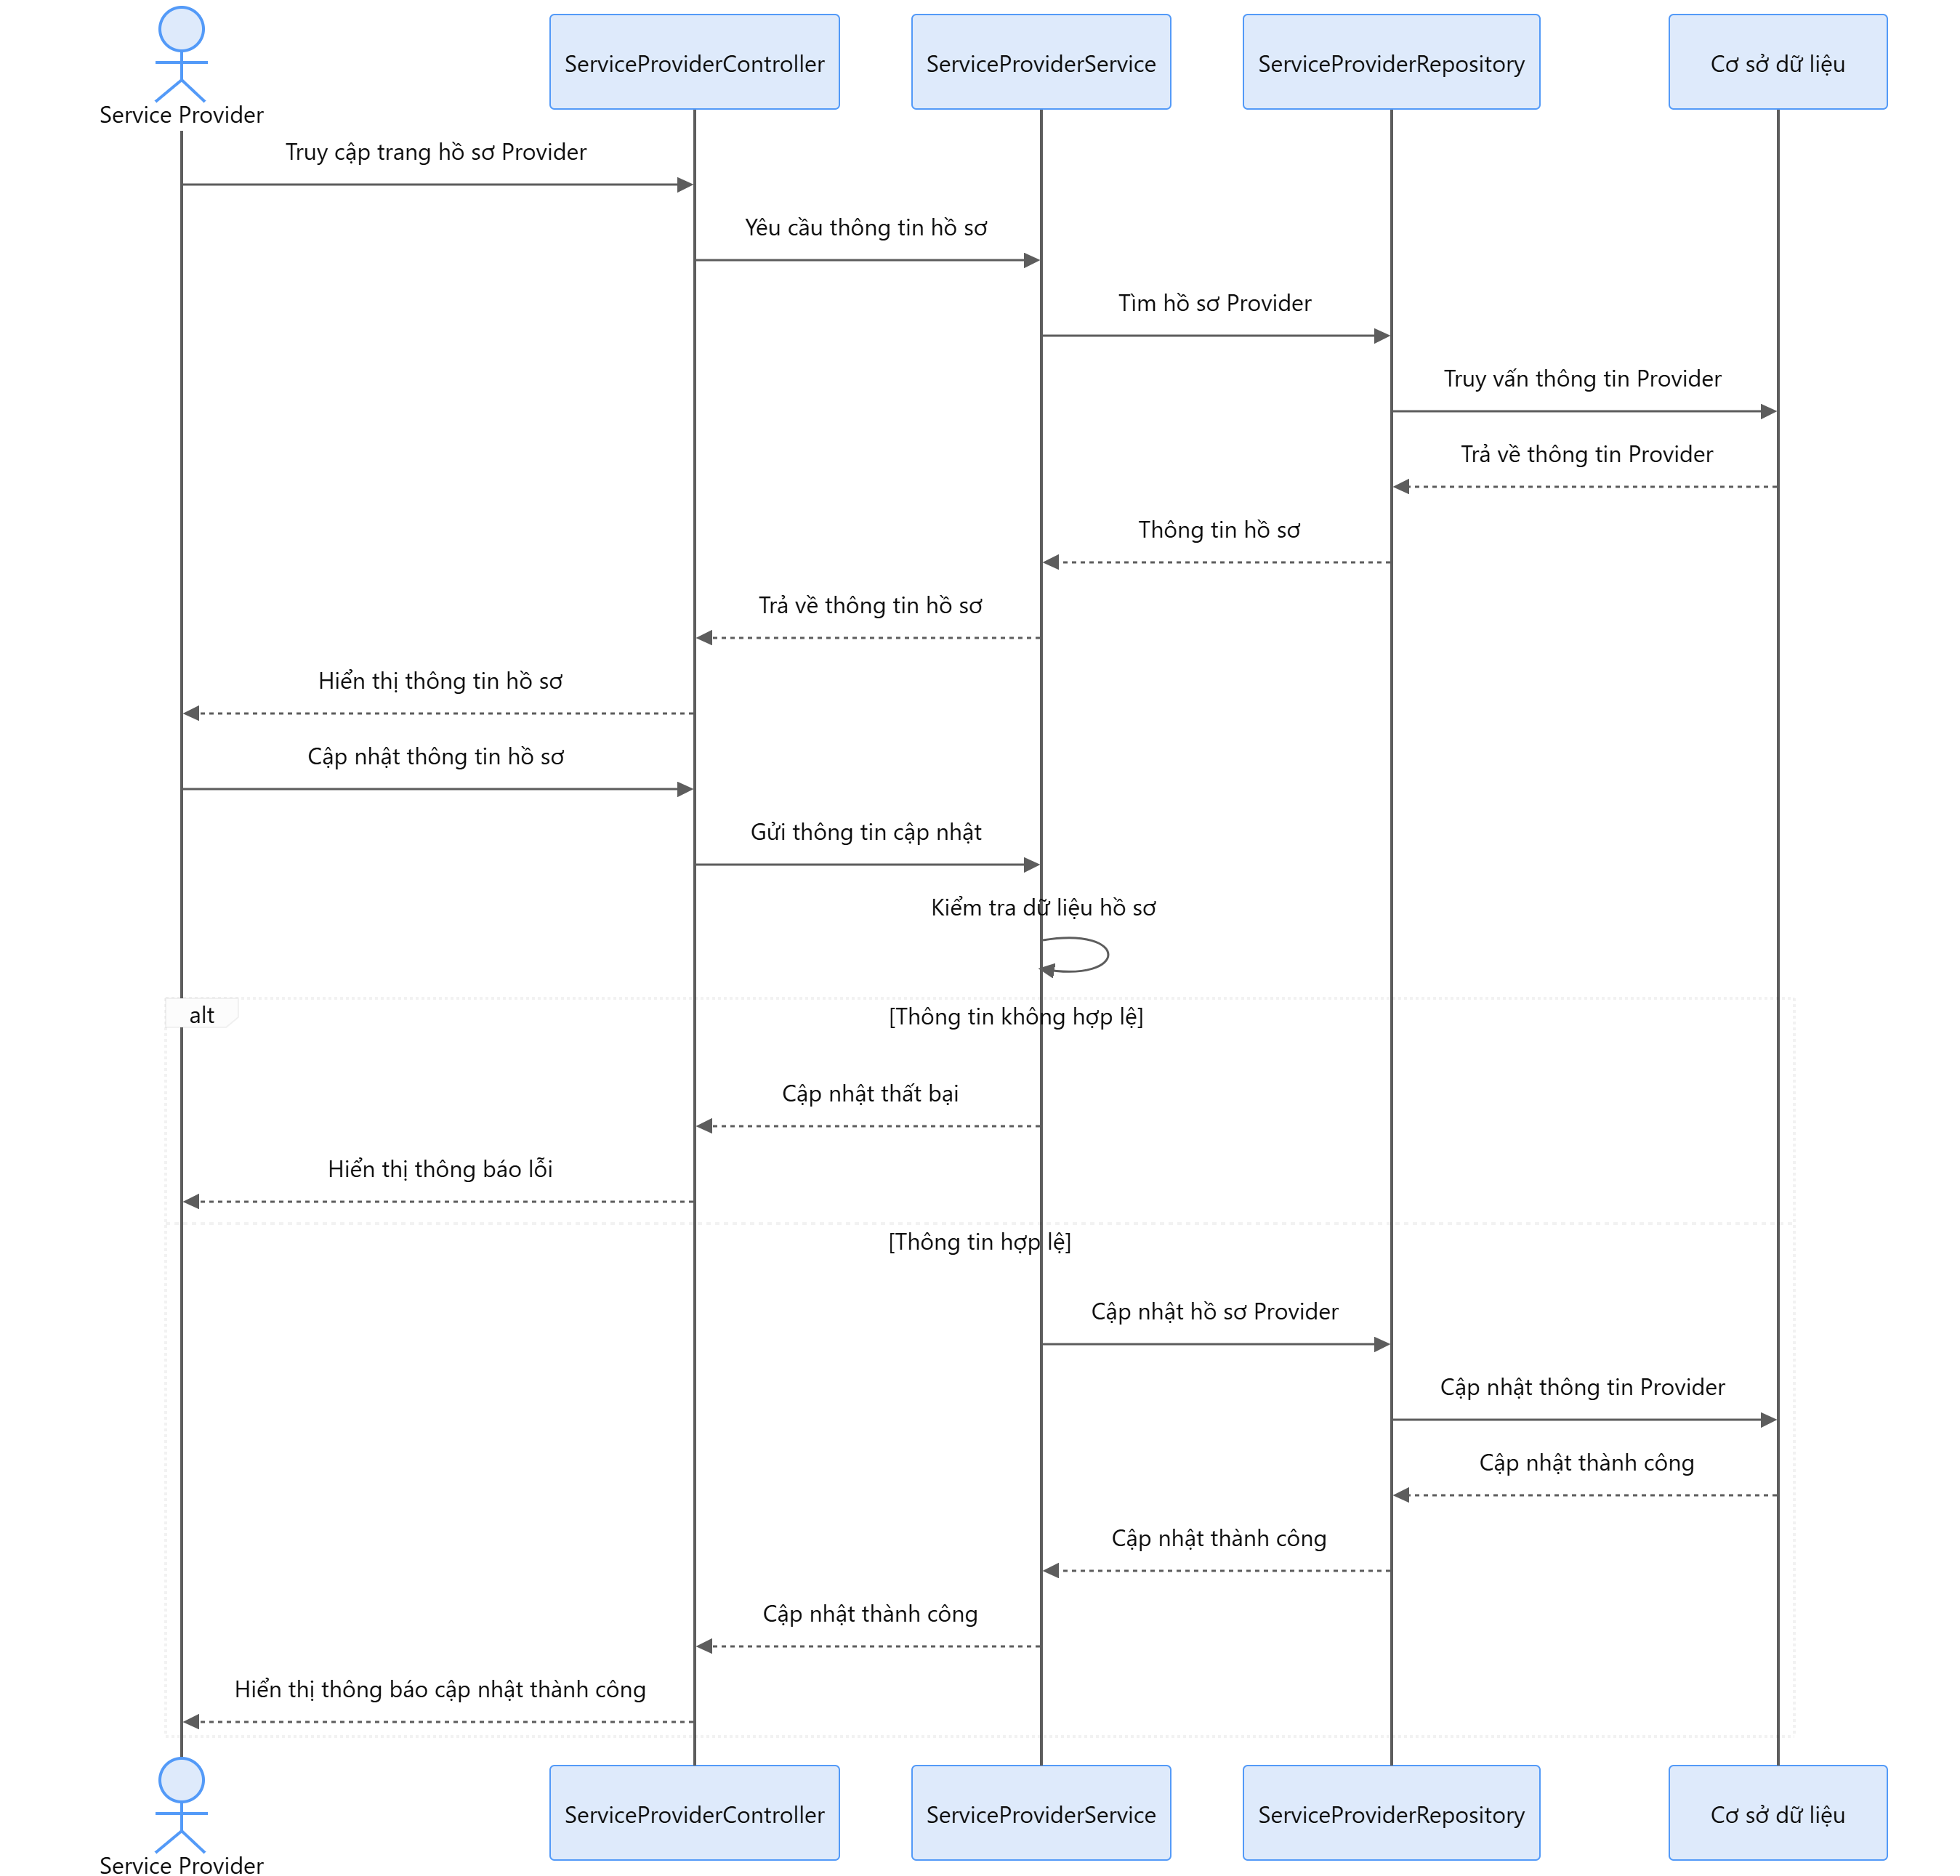
\includegraphics[width=1.1\textwidth]{images/35.png}
\end{figure}


\subsubsection{Quản lý Creative Space}

\paragraph{Class Diagram}

\begin{figure}[H]
	\centering
	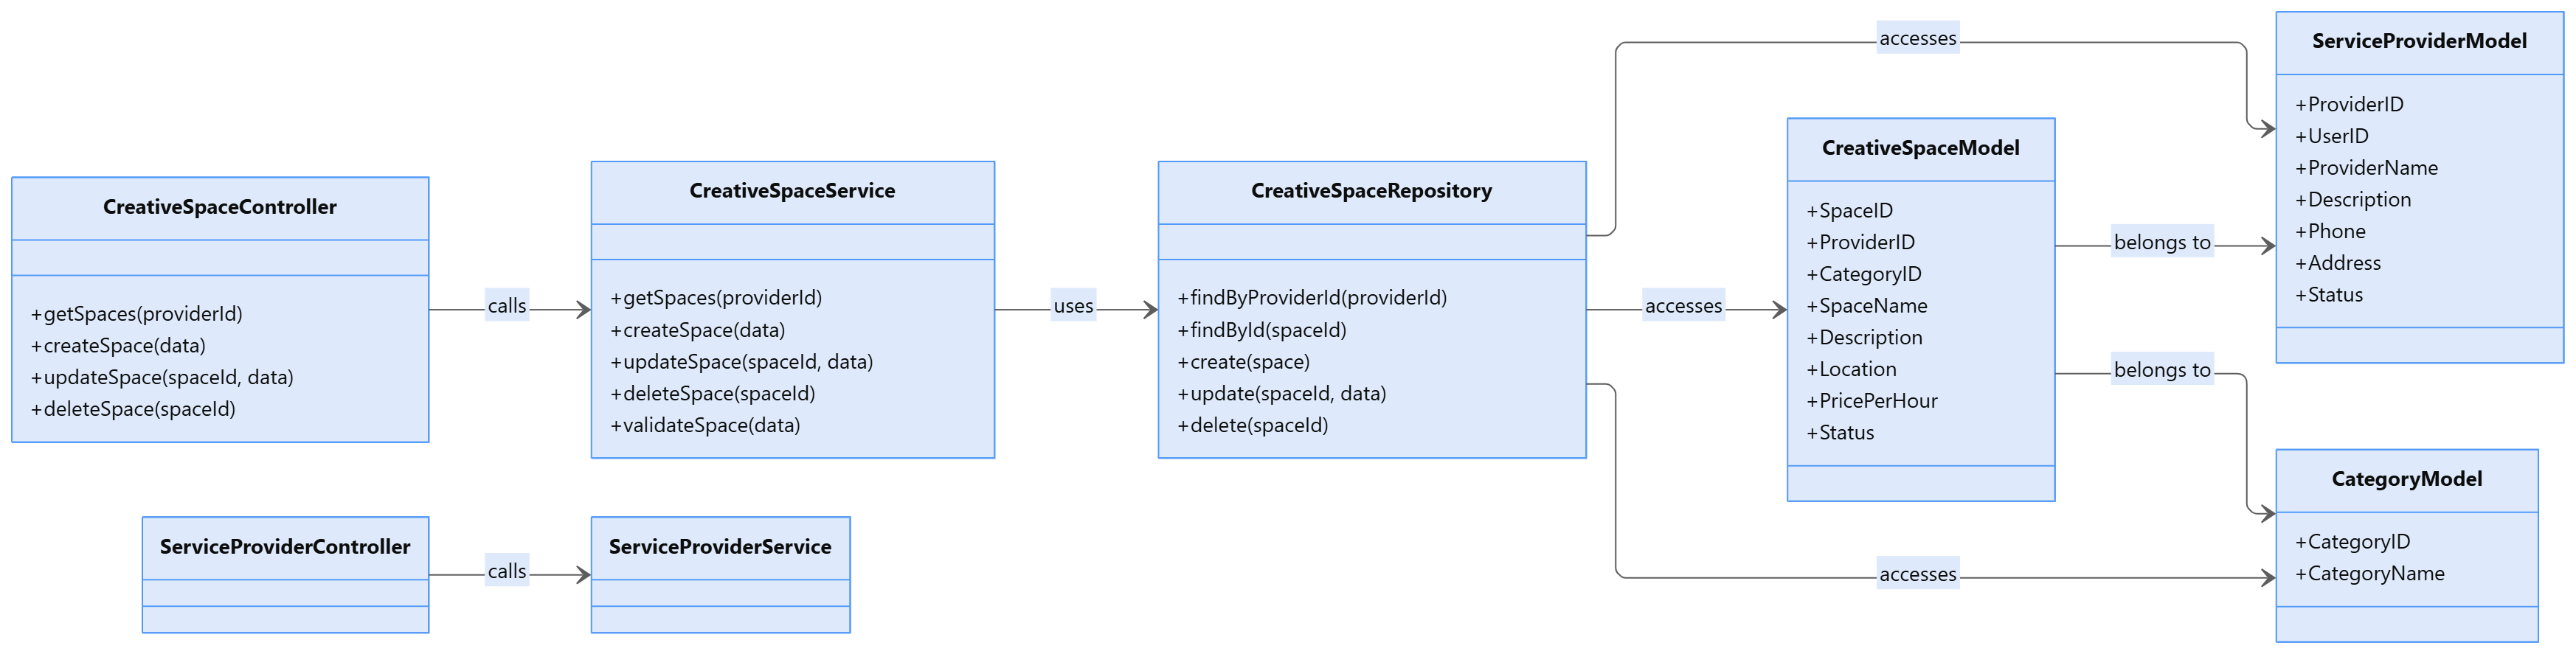
\includegraphics[width=1.1\textwidth]{images/36.png}
\end{figure}

\paragraph{Sequence Diagram}

\begin{figure}[H]
	\centering
	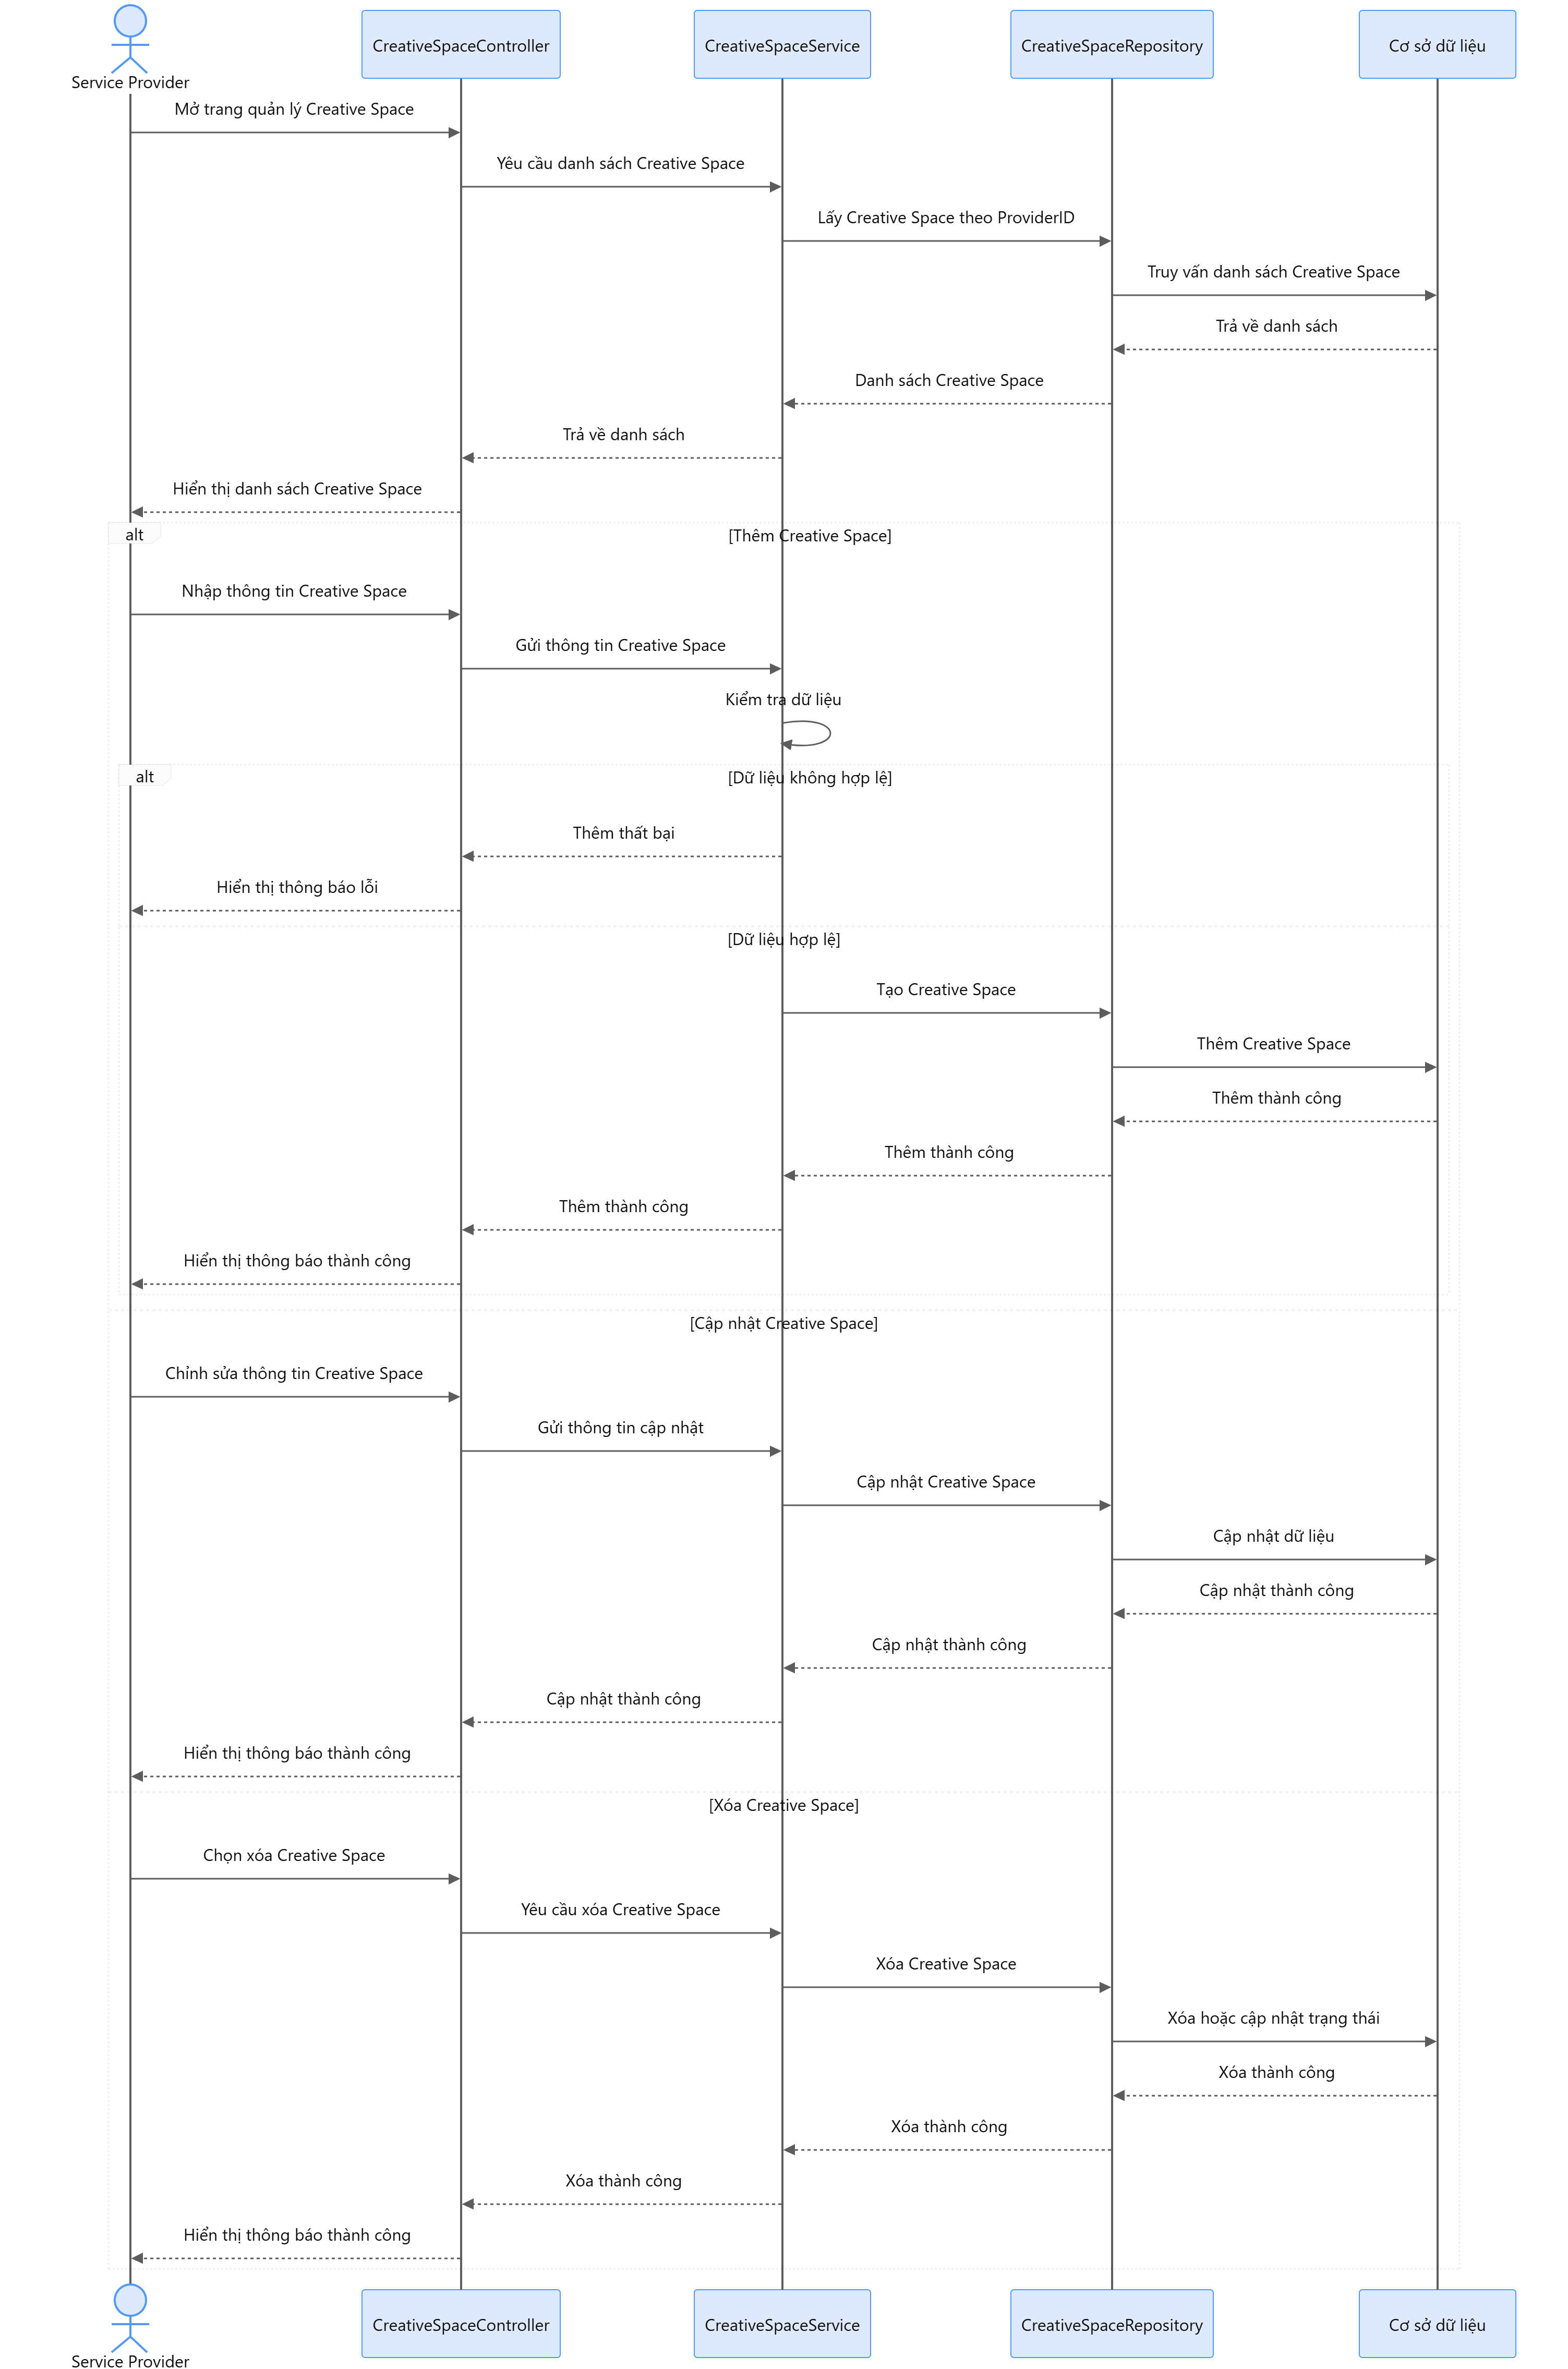
\includegraphics[width=1.1\textwidth]{images/37.png}
\end{figure}


\subsubsection{Quản lý Equipment}

\paragraph{Class Diagram}

\begin{figure}[H]
	\centering
	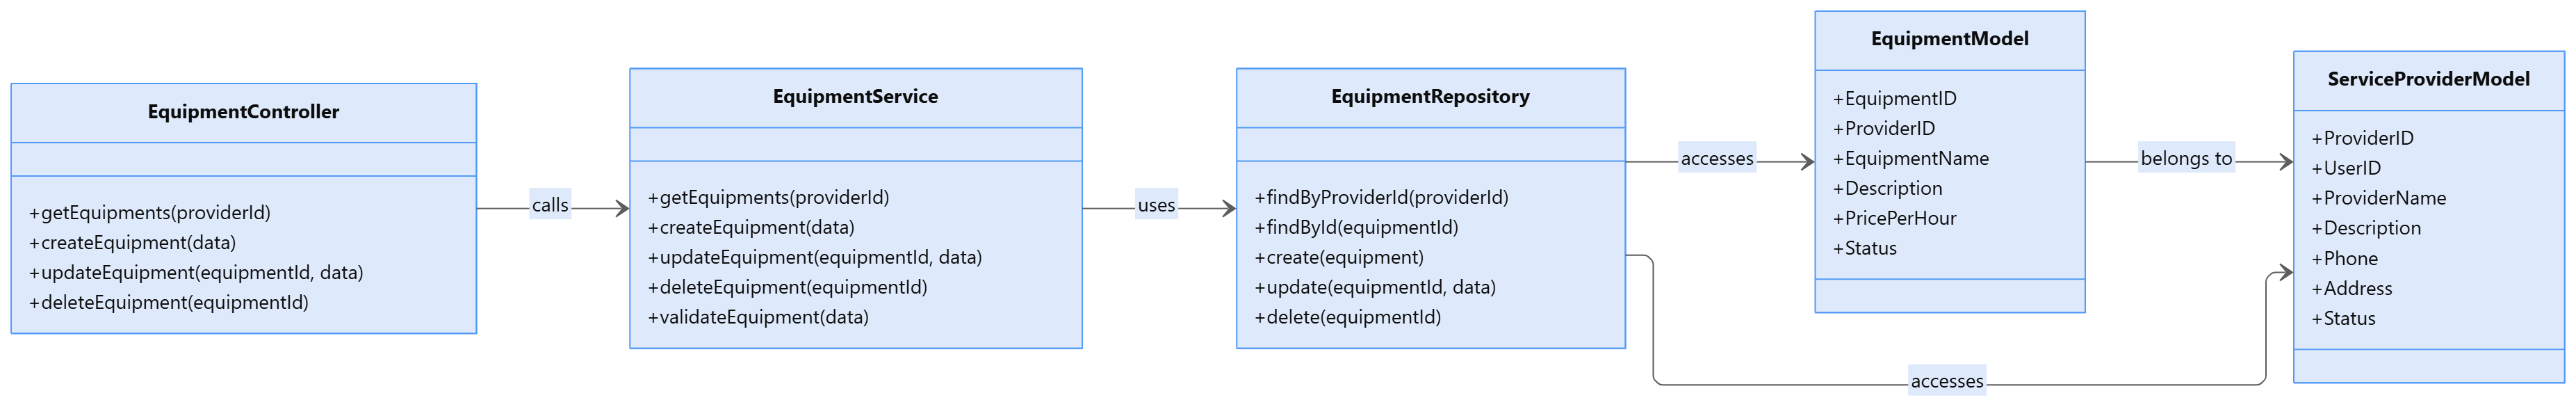
\includegraphics[width=1.1\textwidth]{images/38.png}
\end{figure}

\paragraph{Sequence Diagram}

\begin{figure}[H]
	\centering
	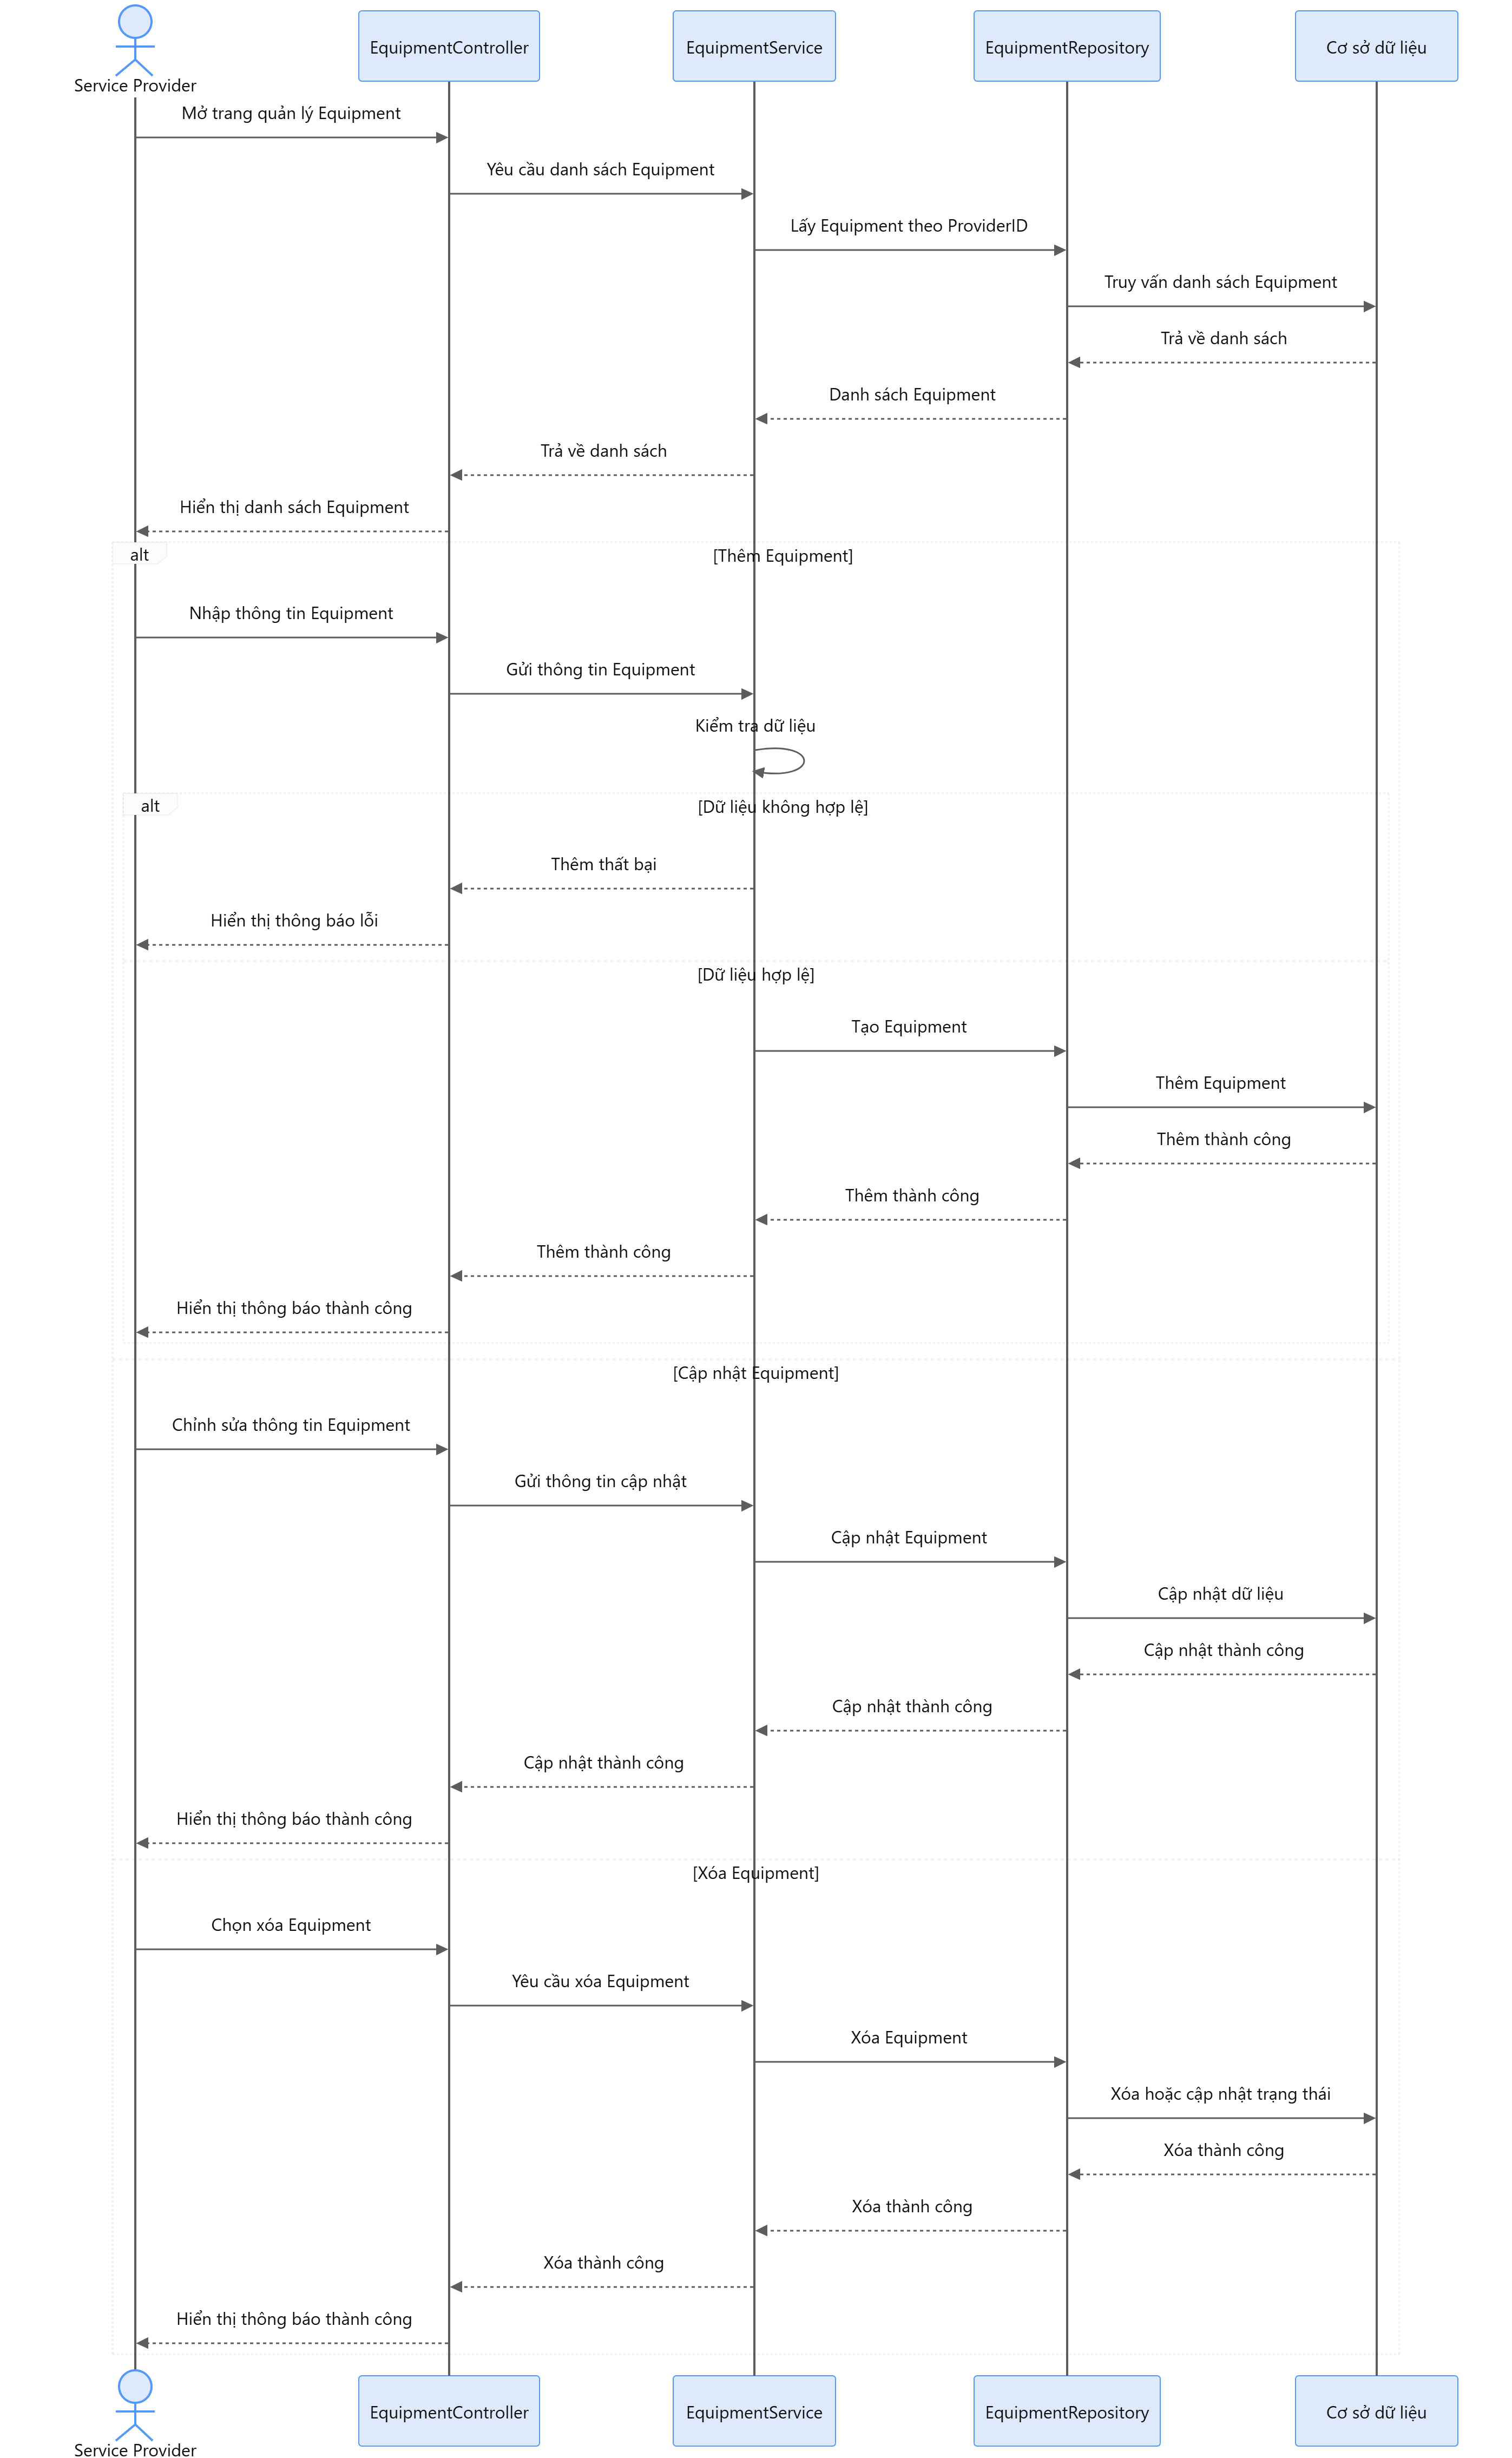
\includegraphics[width=1.1\textwidth]{images/39.png}
\end{figure}


\subsubsection{Quản lý Service Package}

\paragraph{Class Diagram}

\begin{figure}[H]
	\centering
	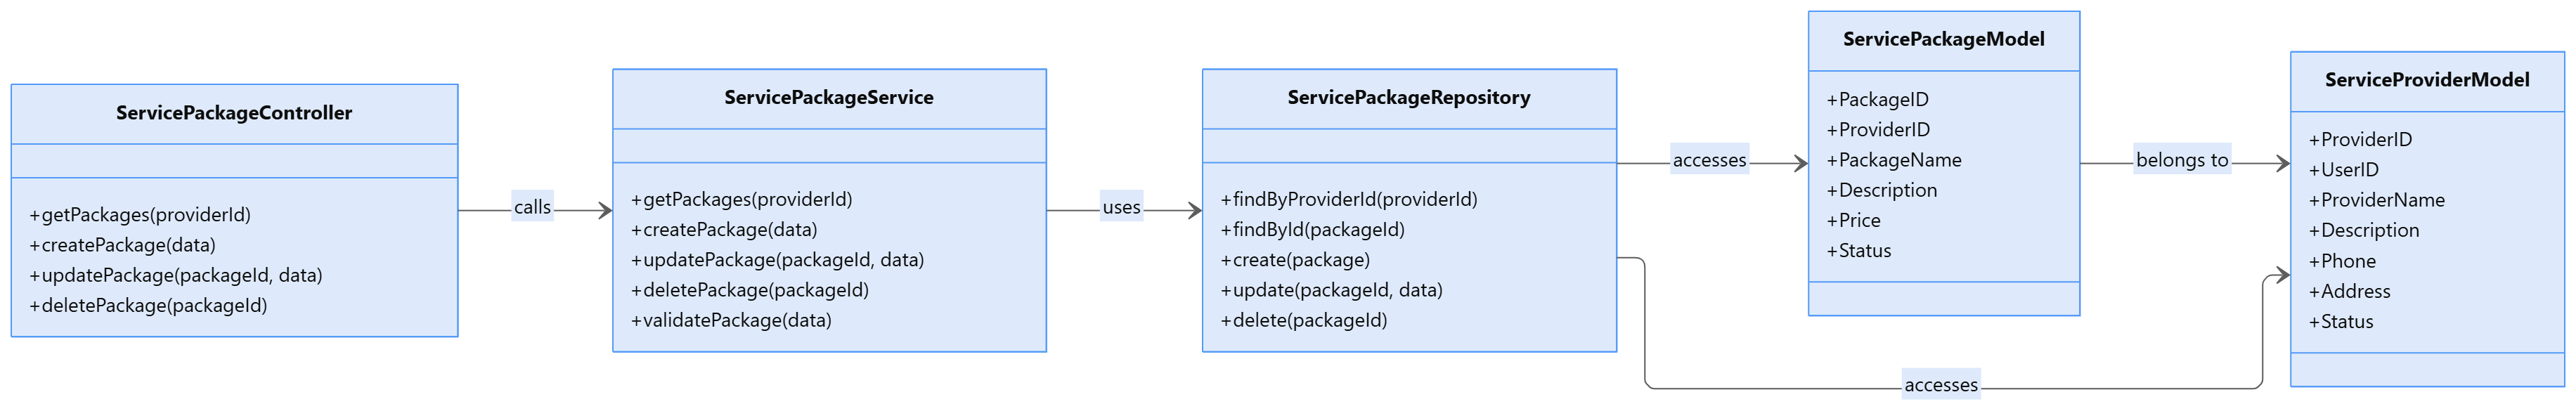
\includegraphics[width=1.1\textwidth]{images/40.png}
\end{figure}

\paragraph{Sequence Diagram}

\begin{figure}[H]
	\centering
	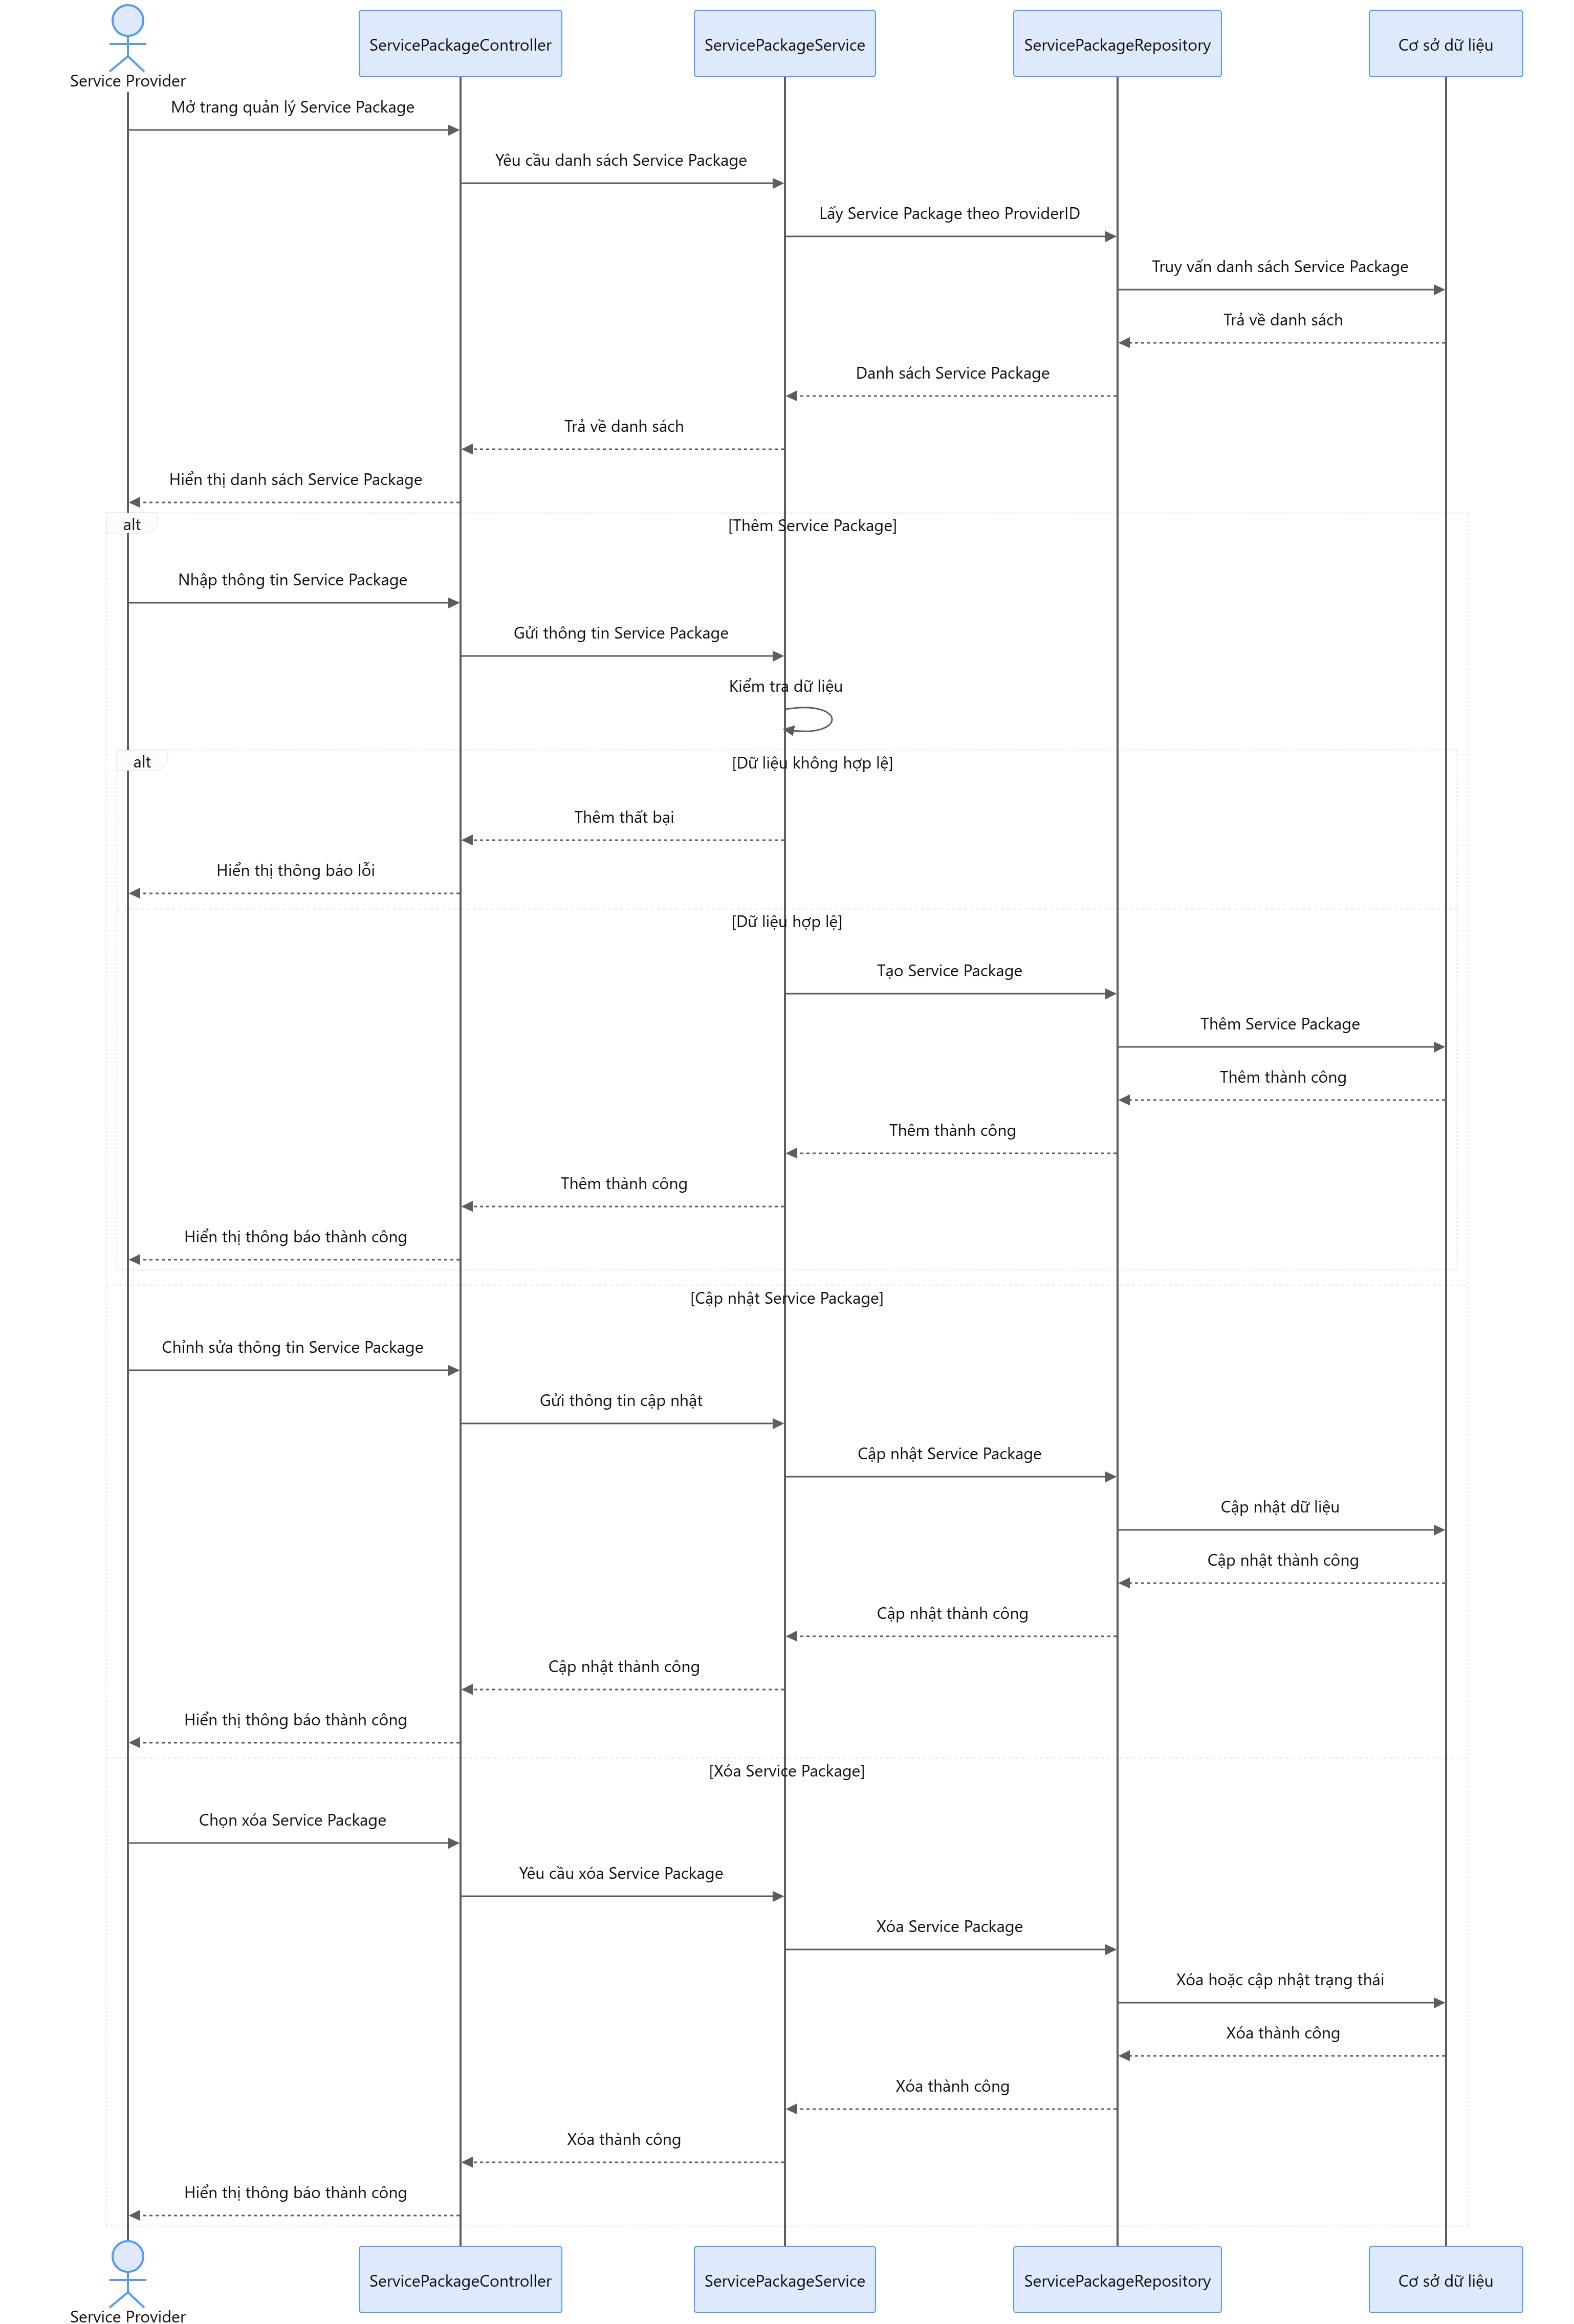
\includegraphics[width=1.1\textwidth]{images/41.png}
\end{figure}


\subsubsection{Quản lý Booking}

\paragraph{Class Diagram}

\begin{figure}[H]
	\centering
	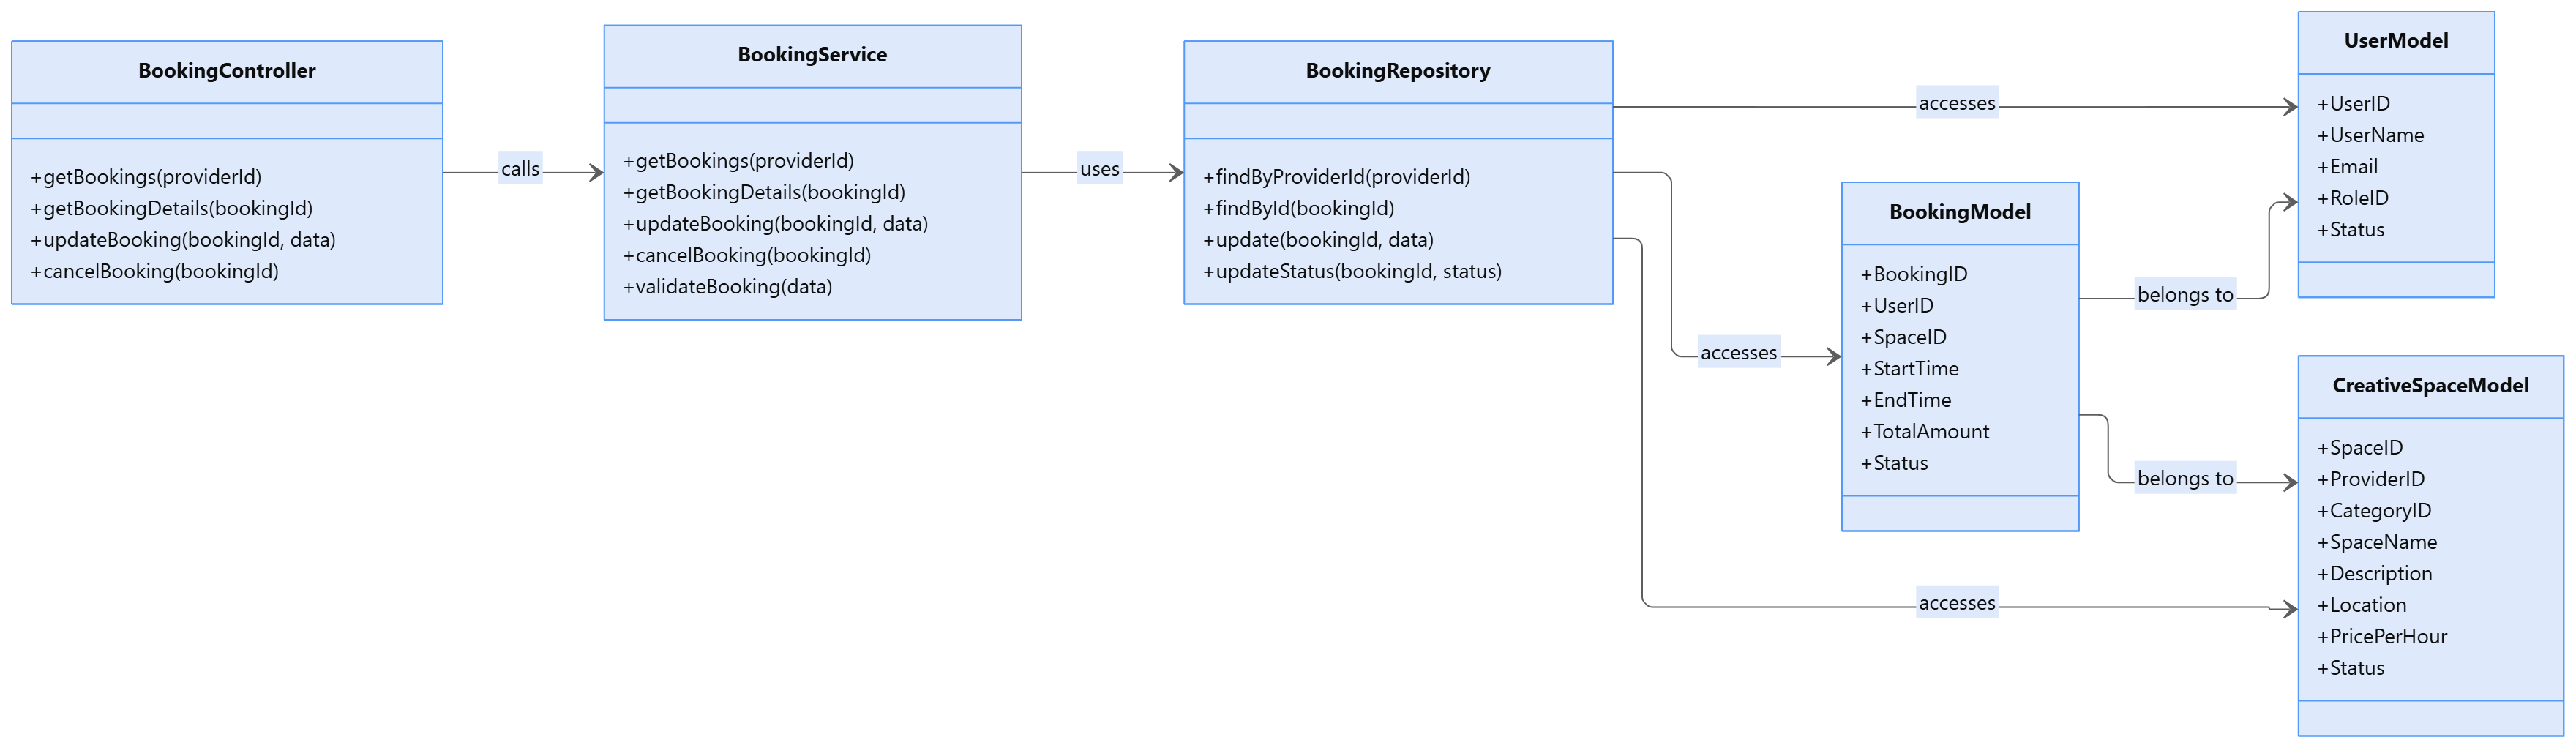
\includegraphics[width=1.1\textwidth]{images/42.png}
\end{figure}

\paragraph{Sequence Diagram}

\begin{figure}[H]
	\centering
	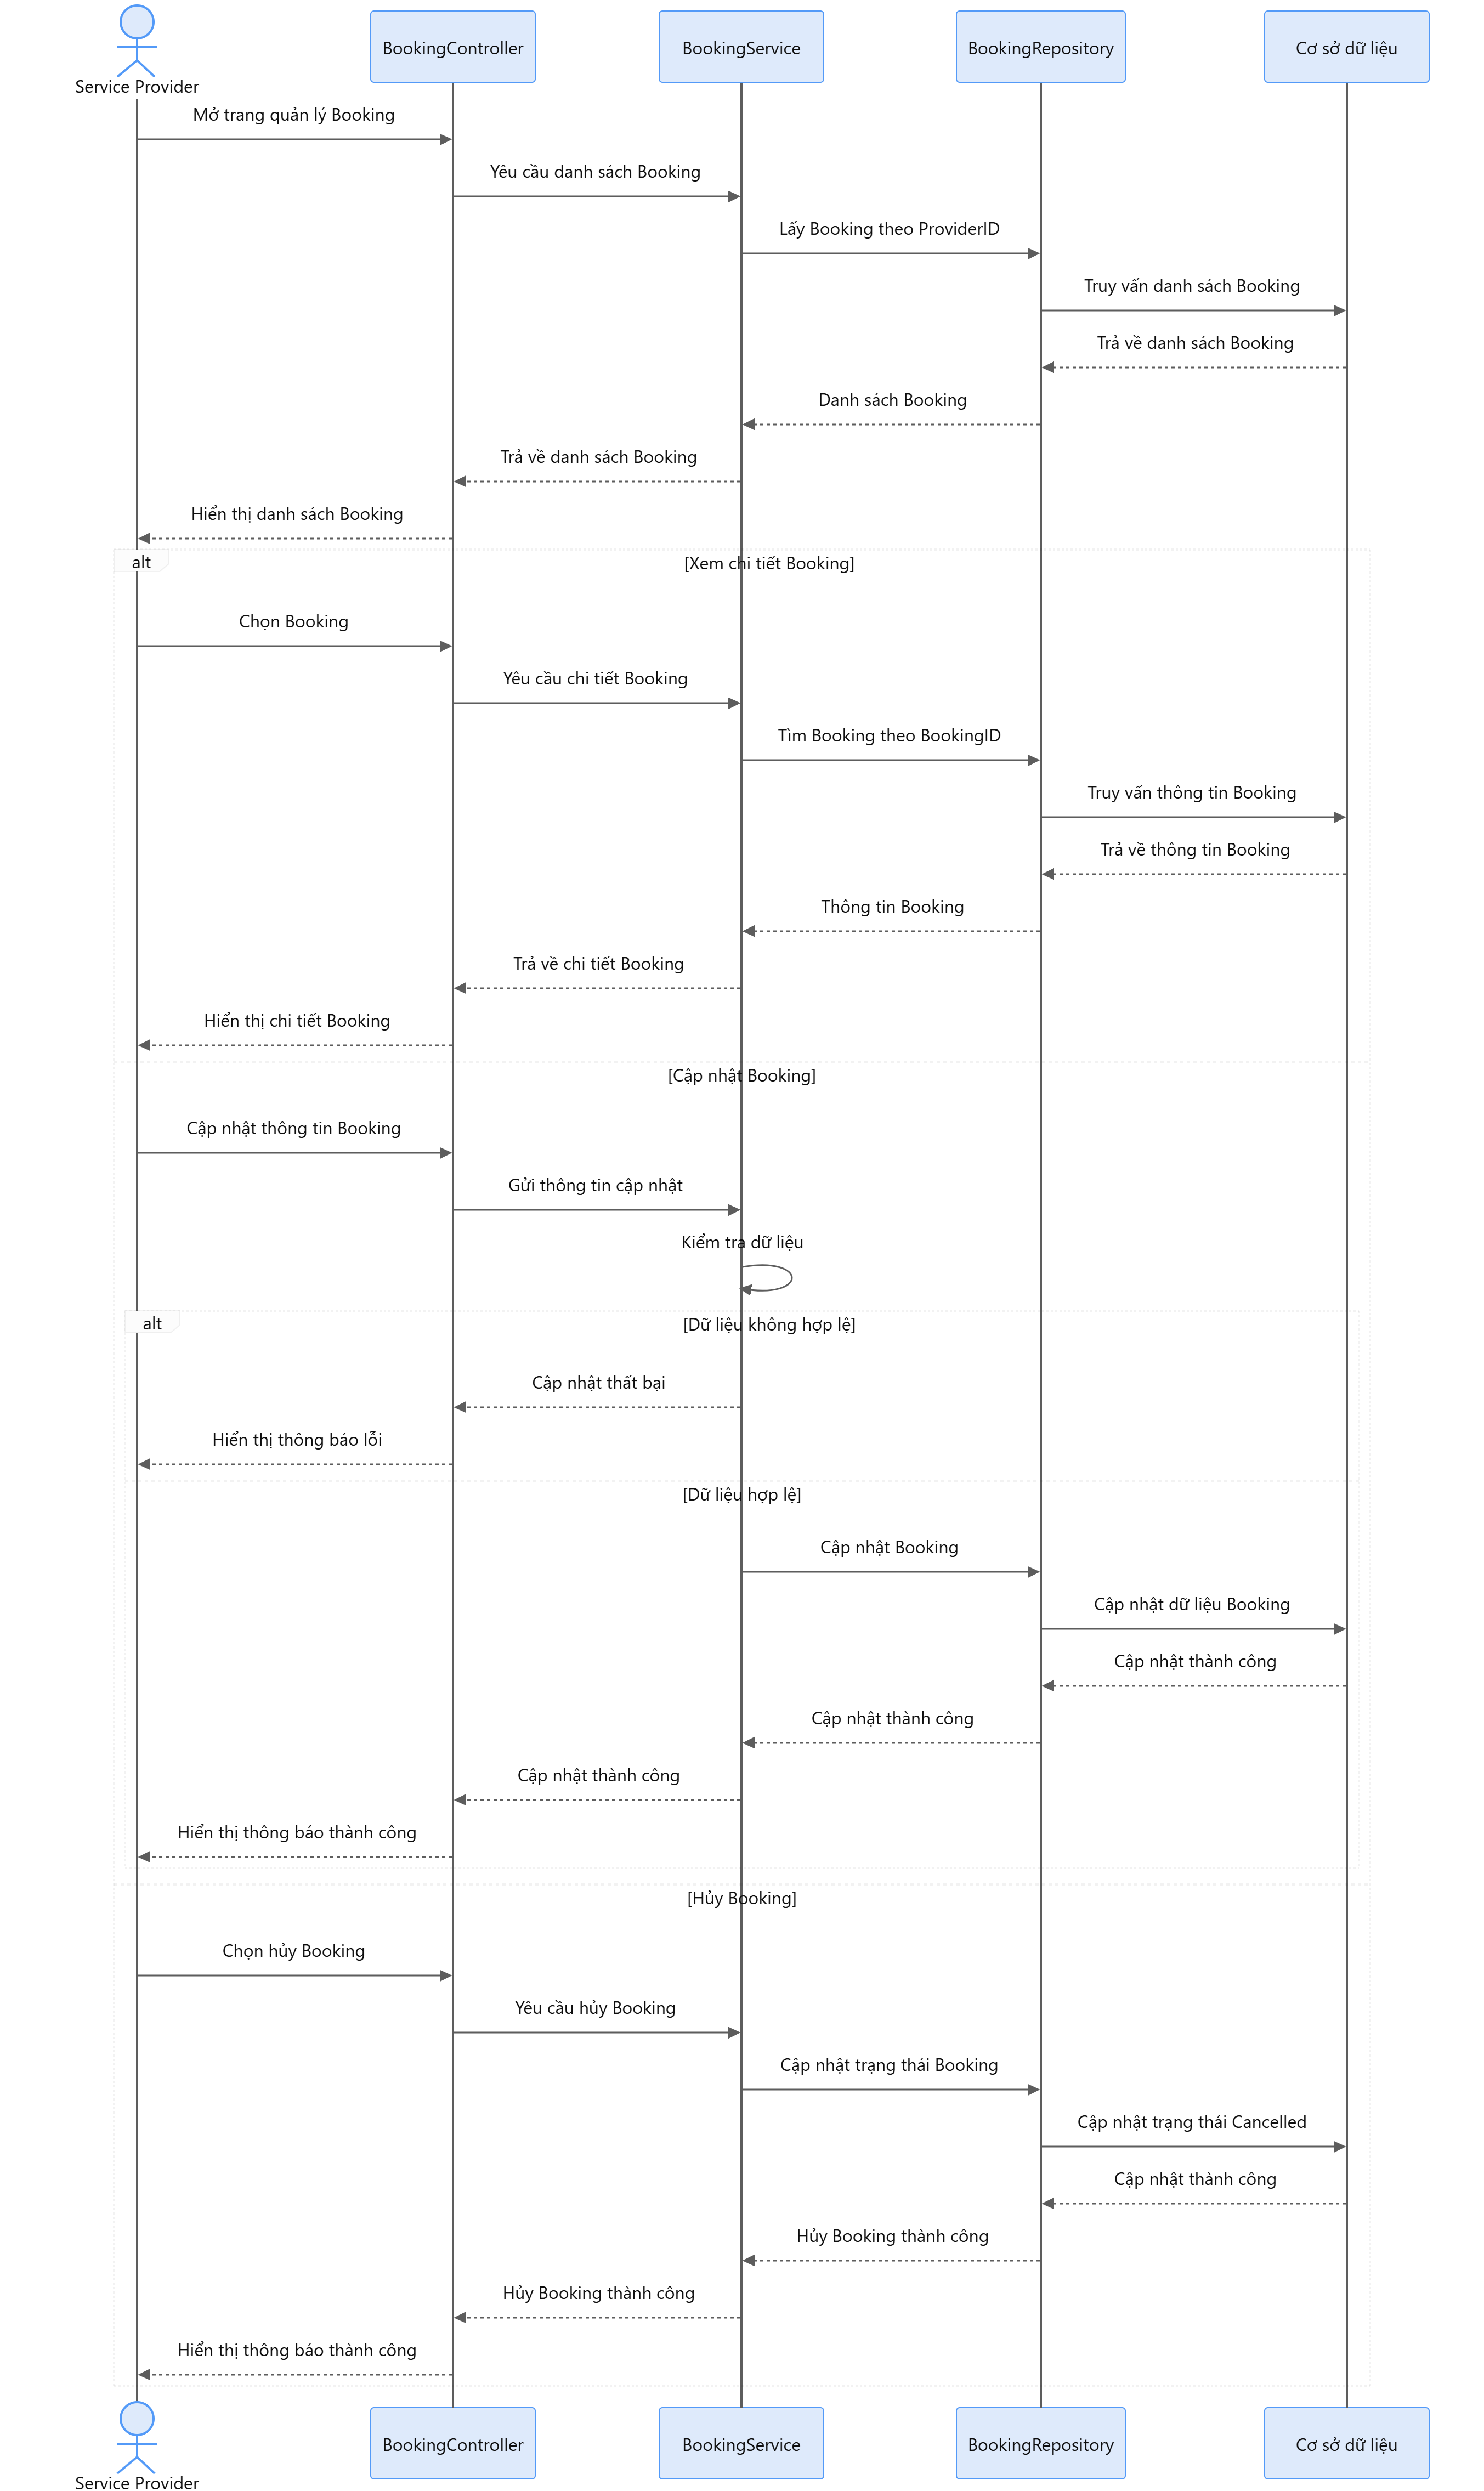
\includegraphics[width=1.1\textwidth]{images/43.png}
\end{figure}


\subsubsection{Xác nhận/Từ chối Booking}

\paragraph{Class Diagram}

\begin{figure}[H]
	\centering
	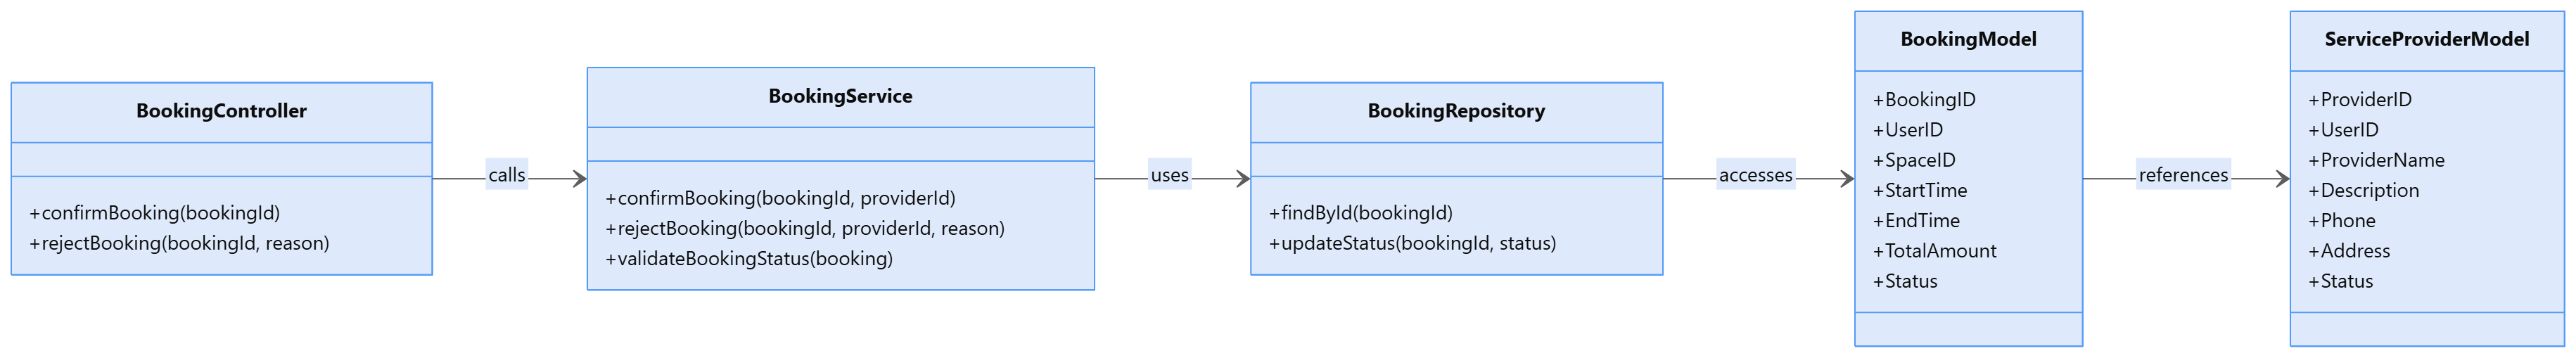
\includegraphics[width=1.1\textwidth]{images/44.png}
\end{figure}

\paragraph{Sequence Diagram}

\begin{figure}[H]
	\centering
	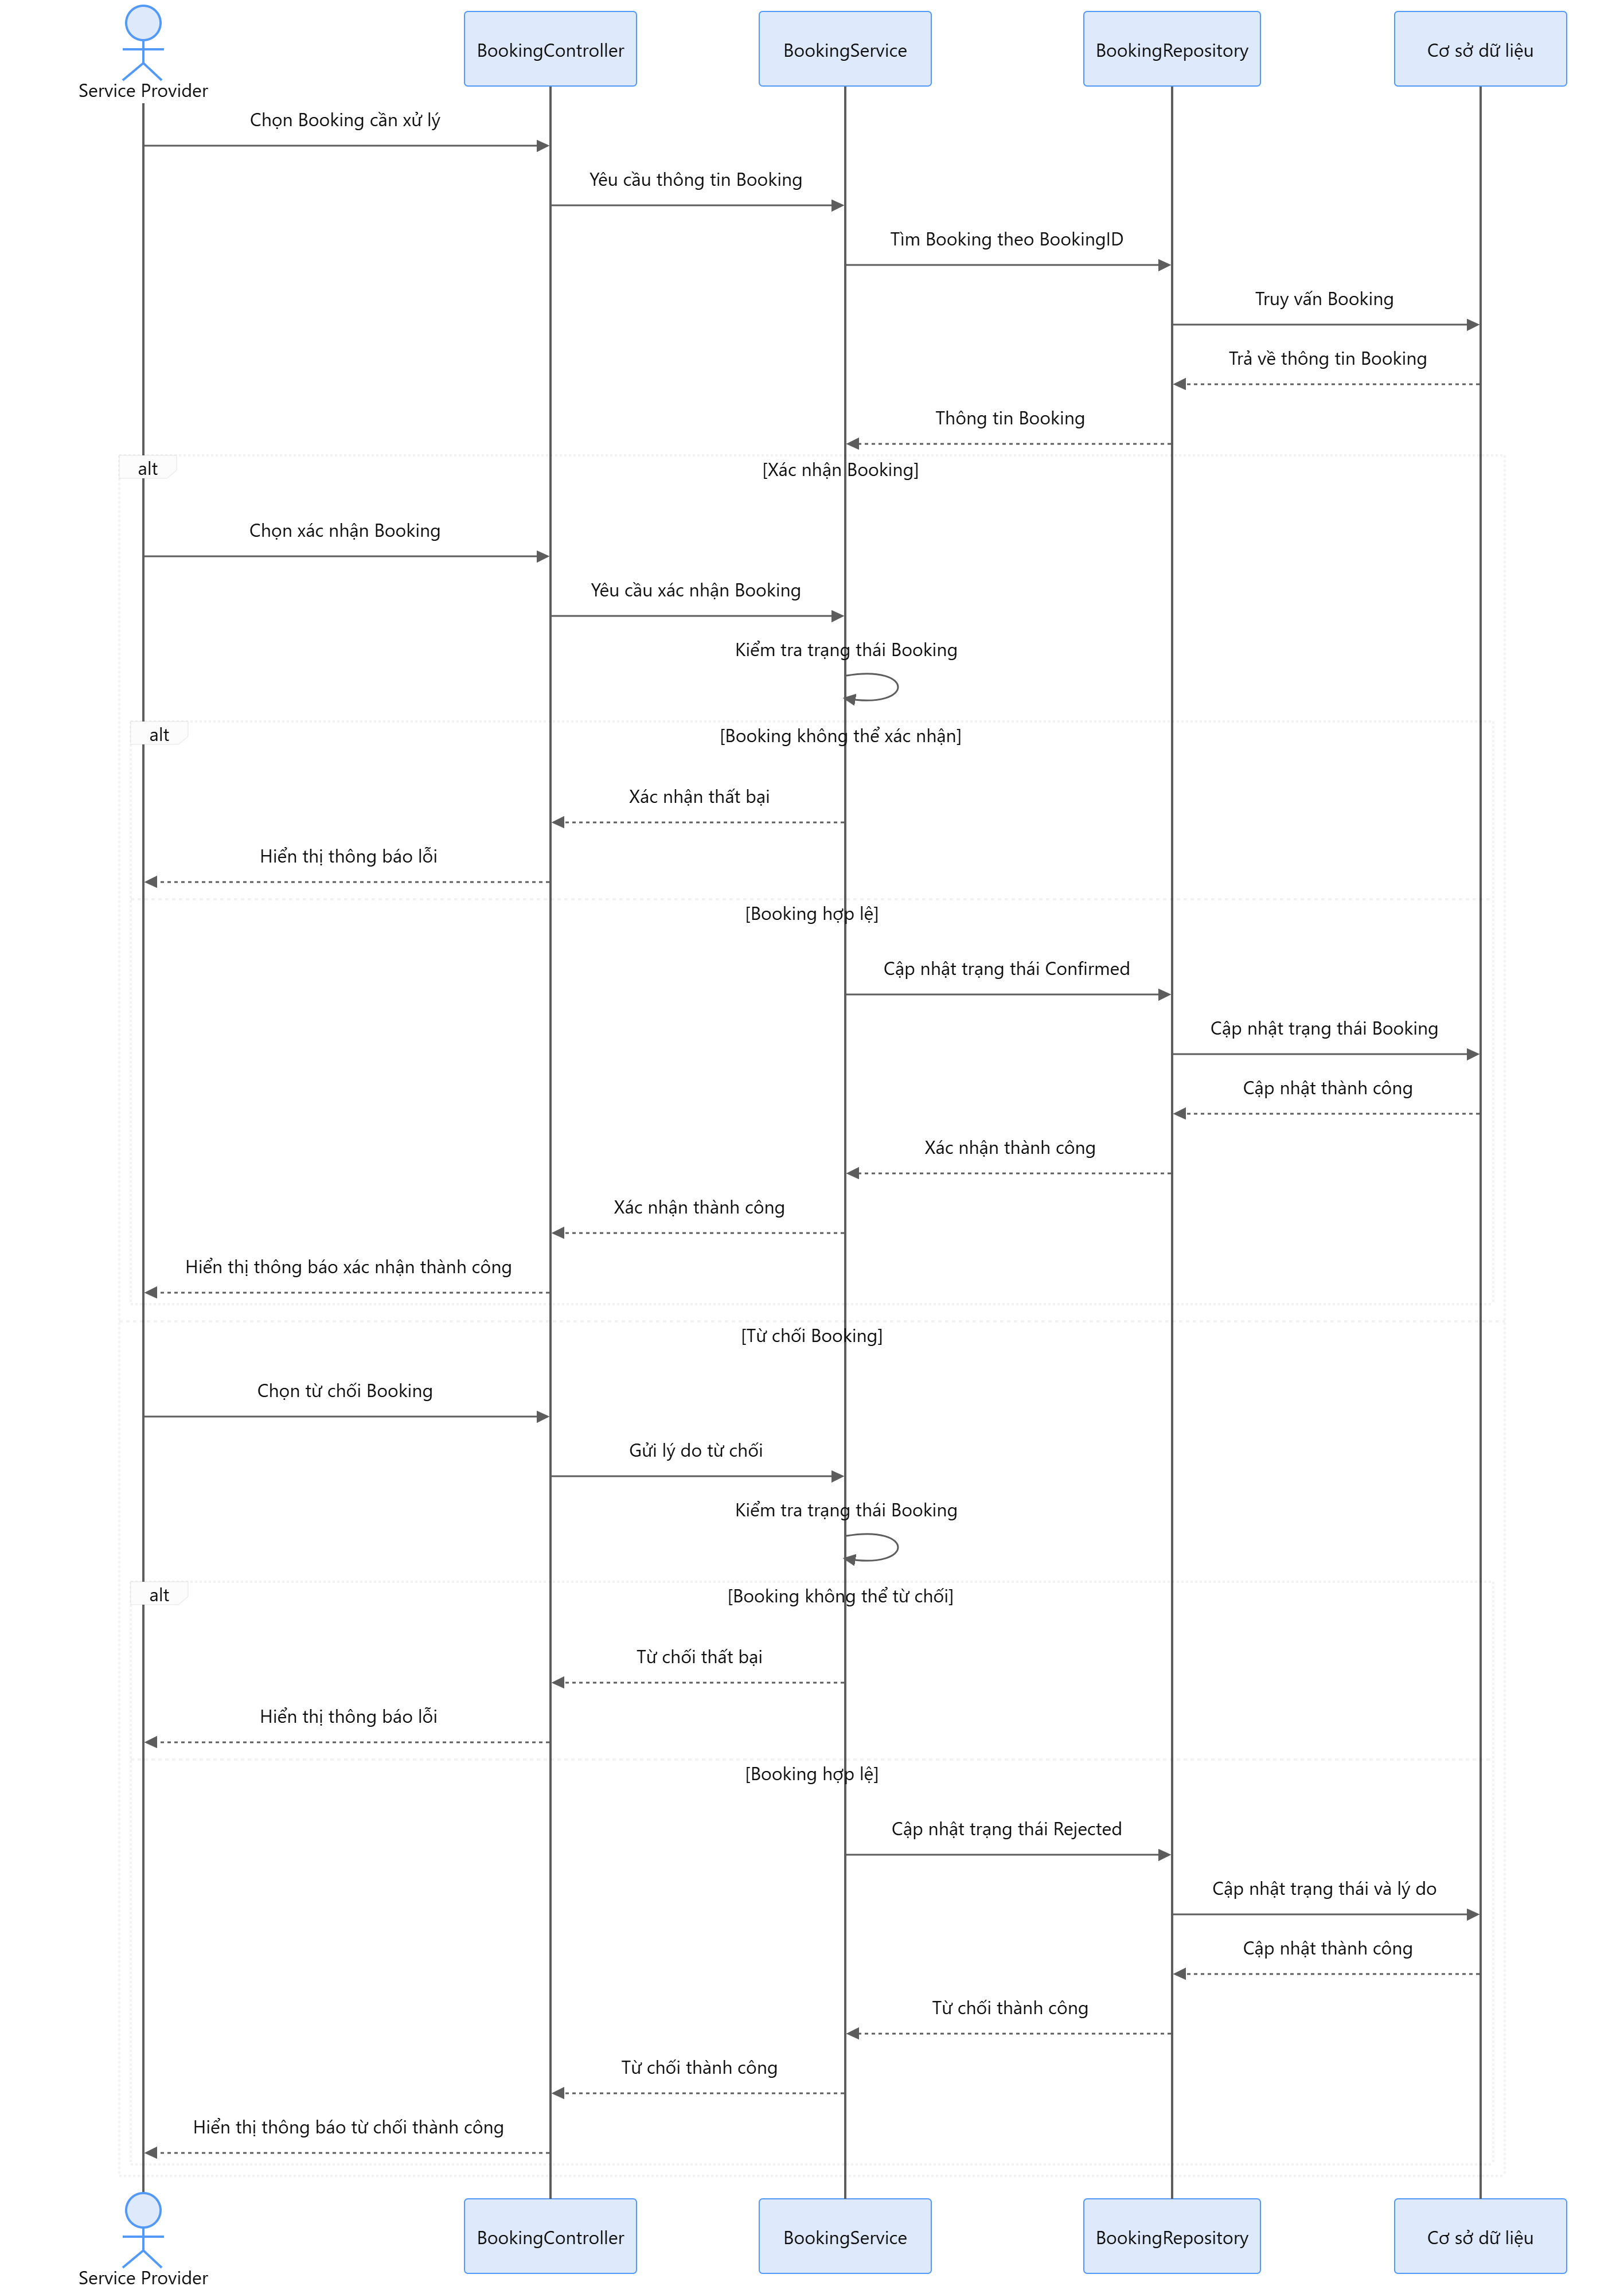
\includegraphics[width=1.1\textwidth]{images/45.png}
\end{figure}


\subsubsection{Quản lý Workshop}

\paragraph{Class Diagram}

\begin{figure}[H]
	\centering
	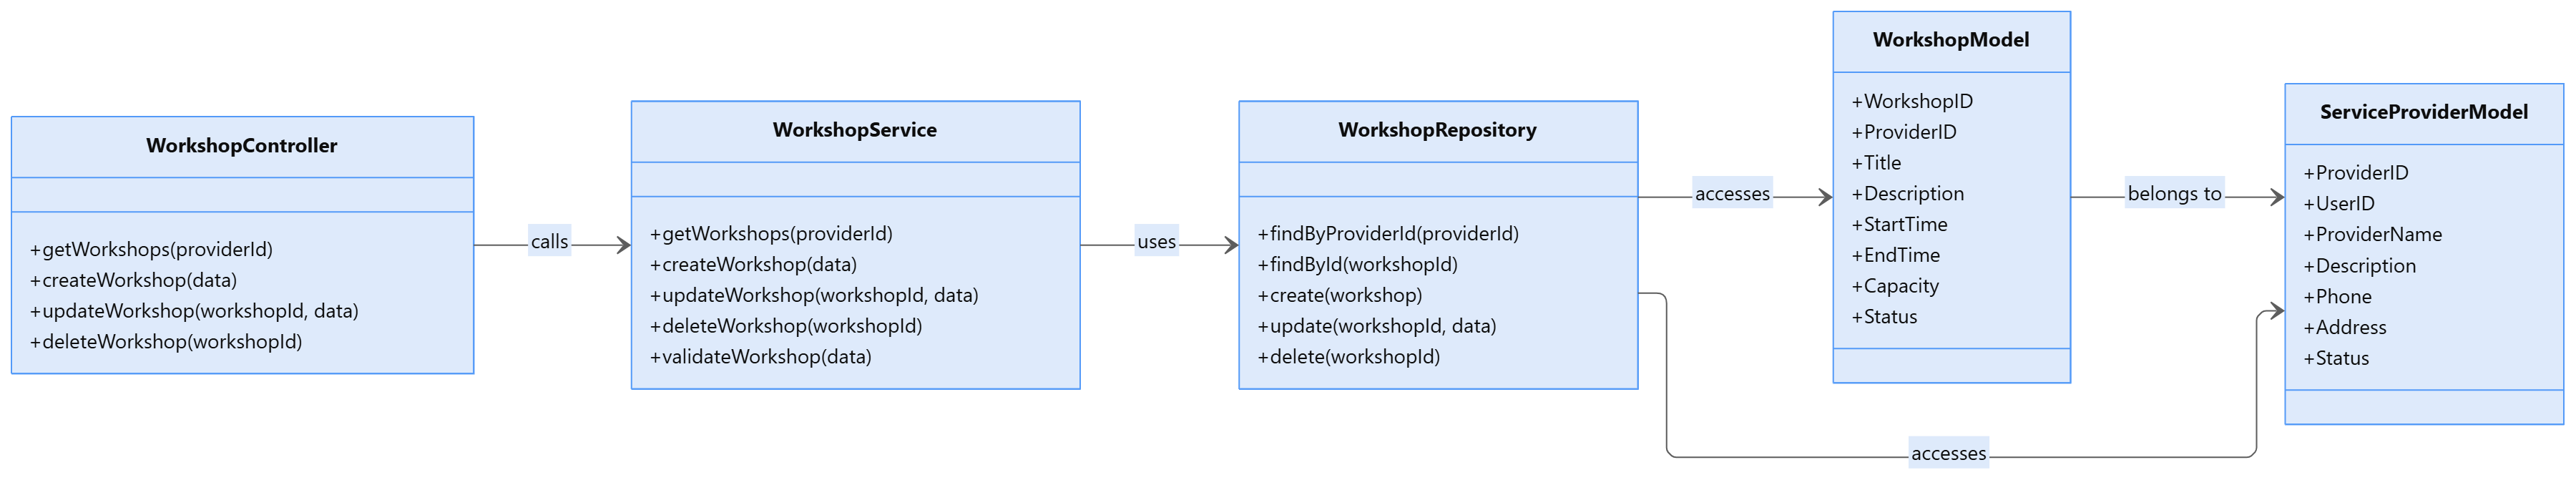
\includegraphics[width=1.1\textwidth]{images/46.png}
\end{figure}

\paragraph{Sequence Diagram}

\begin{figure}[H]
	\centering
	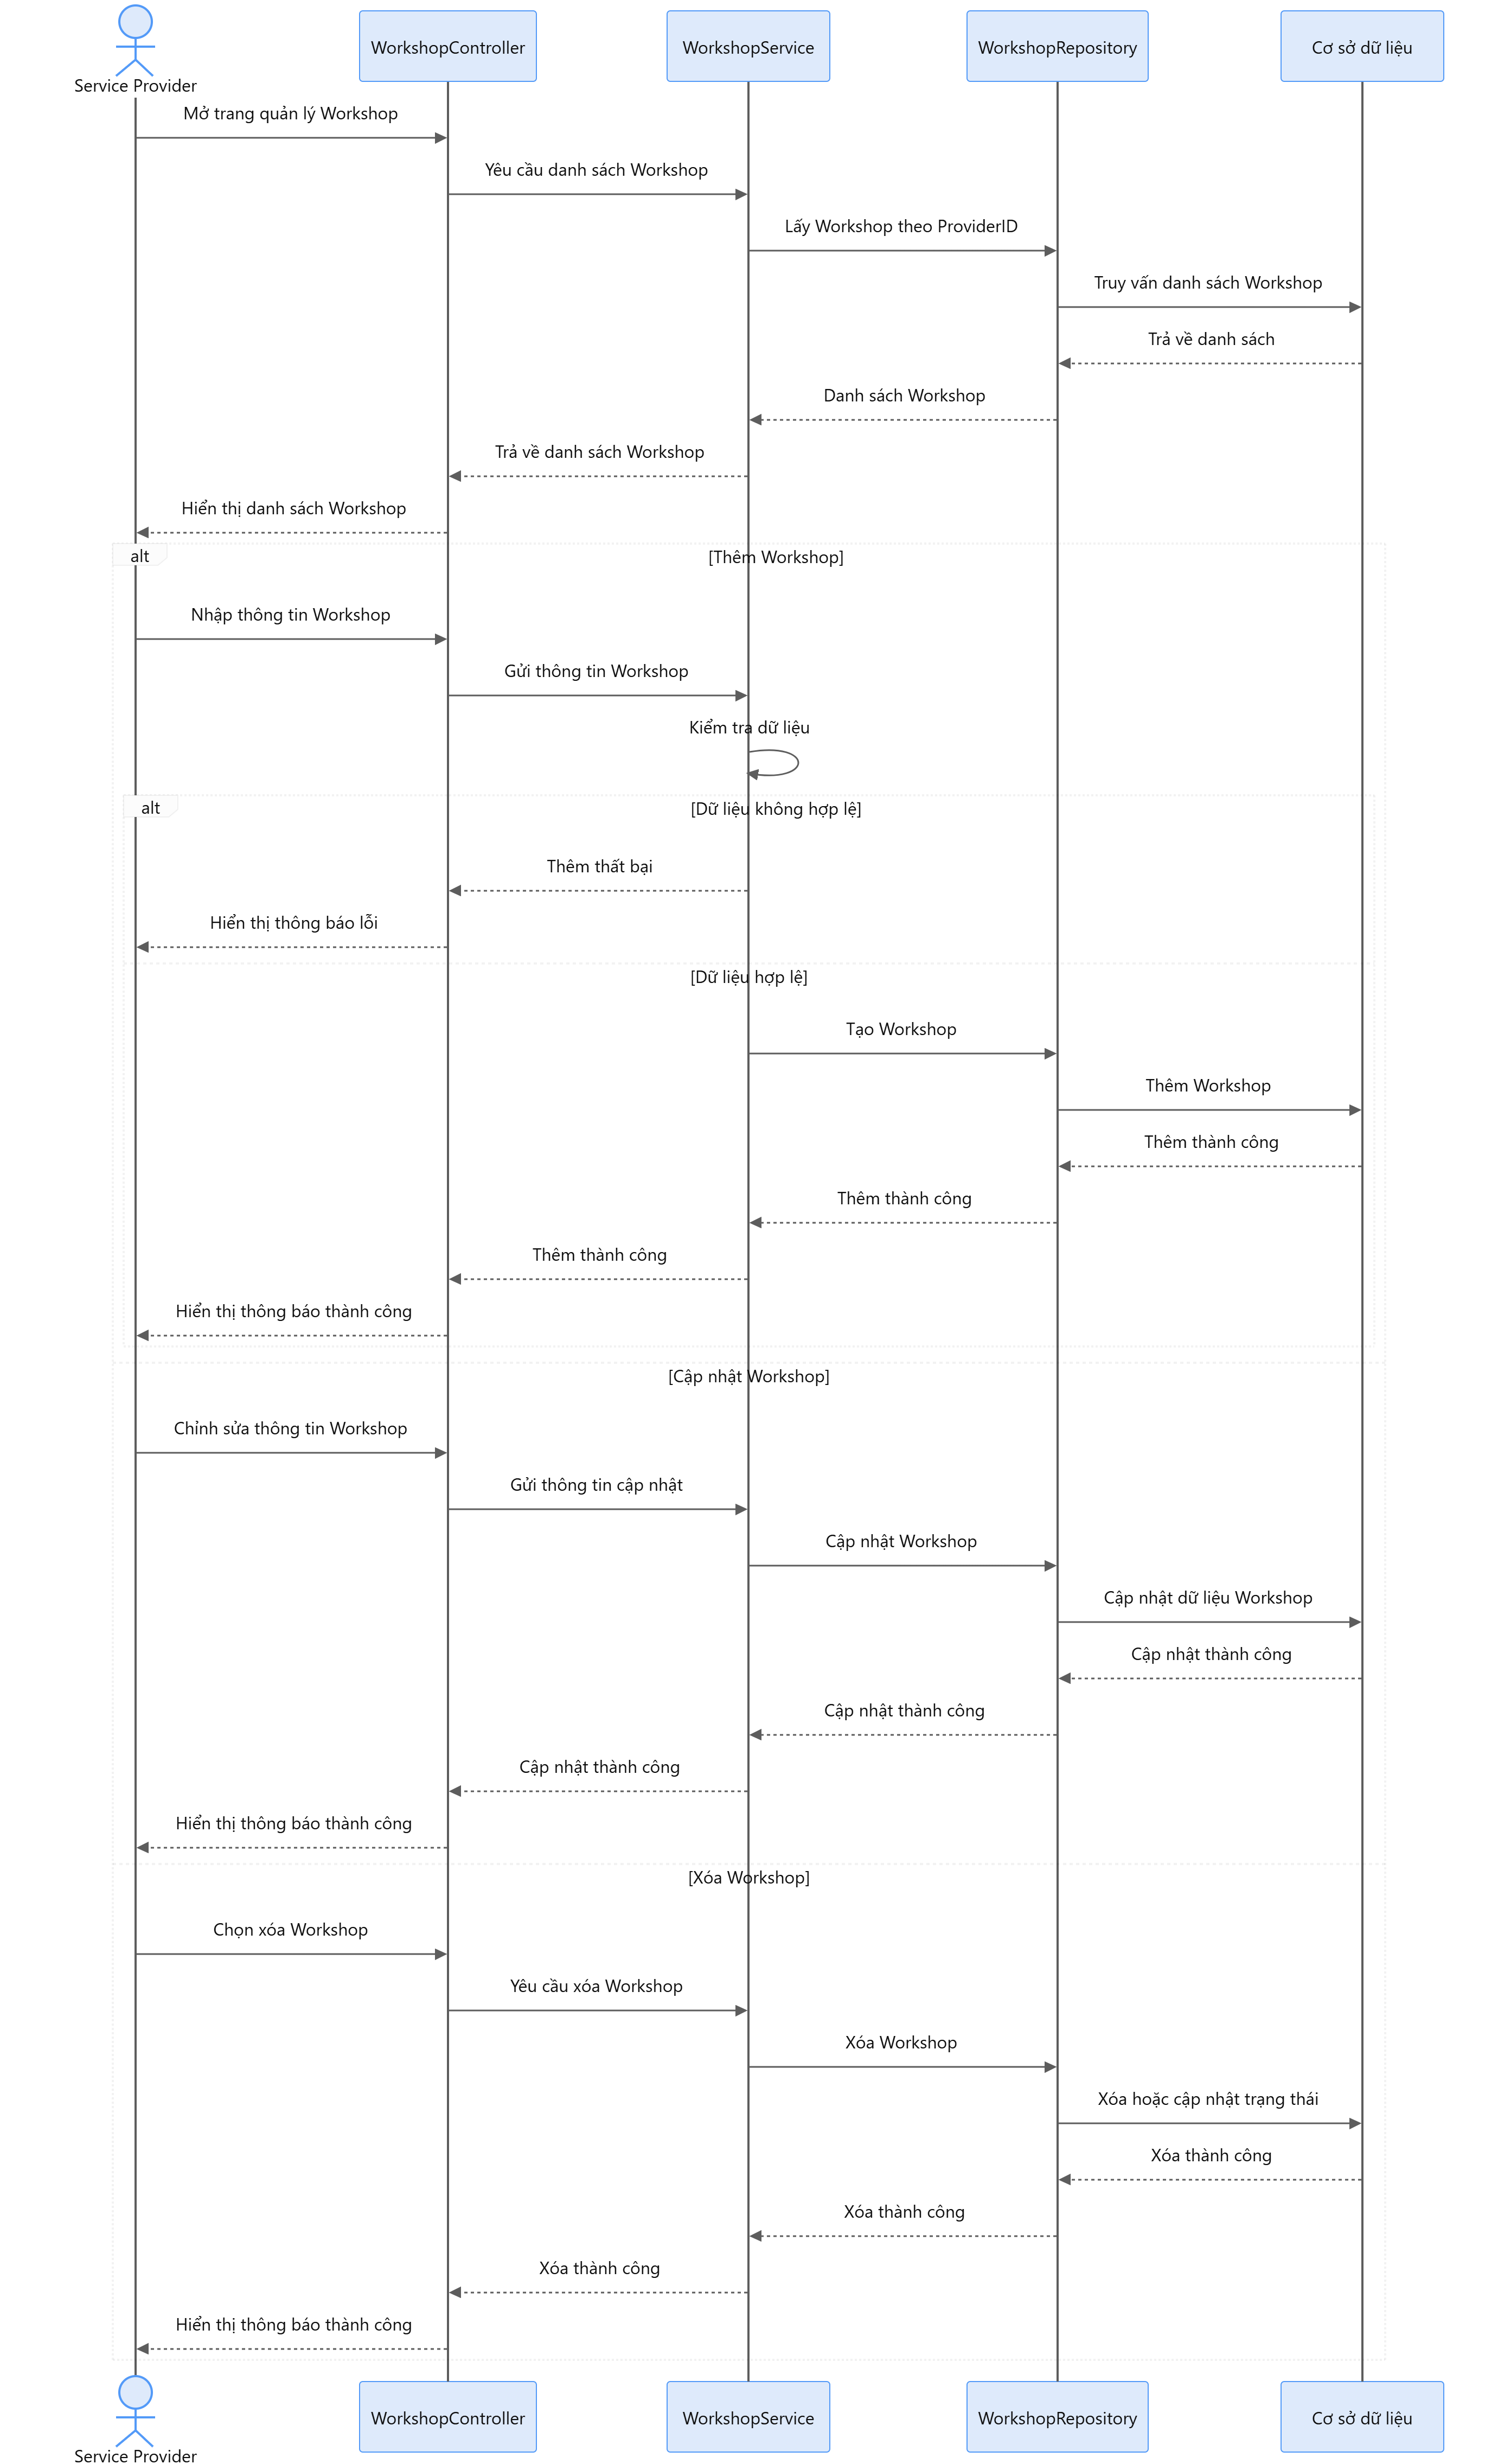
\includegraphics[width=1.1\textwidth]{images/47.png}
\end{figure}


% =========================================================
% 3.8 Administrator Management Module
% =========================================================

\subsection{Administrator Management Module}

\subsubsection{Quản lý người dùng}

\paragraph{Class Diagram}

\begin{figure}[H]
	\centering
	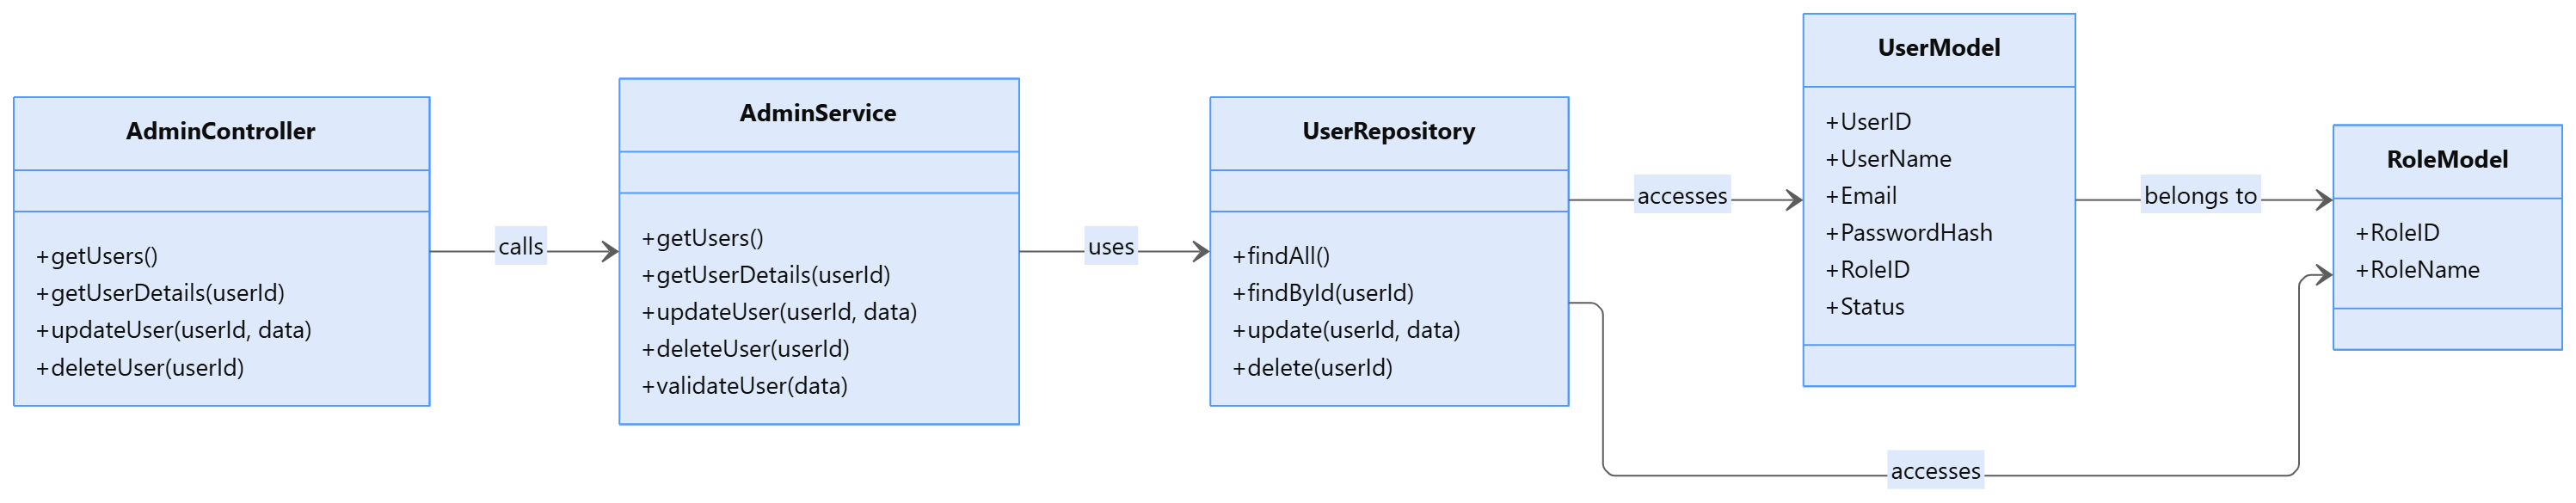
\includegraphics[width=1.1\textwidth]{images/48.png}
\end{figure}

\paragraph{Sequence Diagram}

\begin{figure}[H]
	\centering
	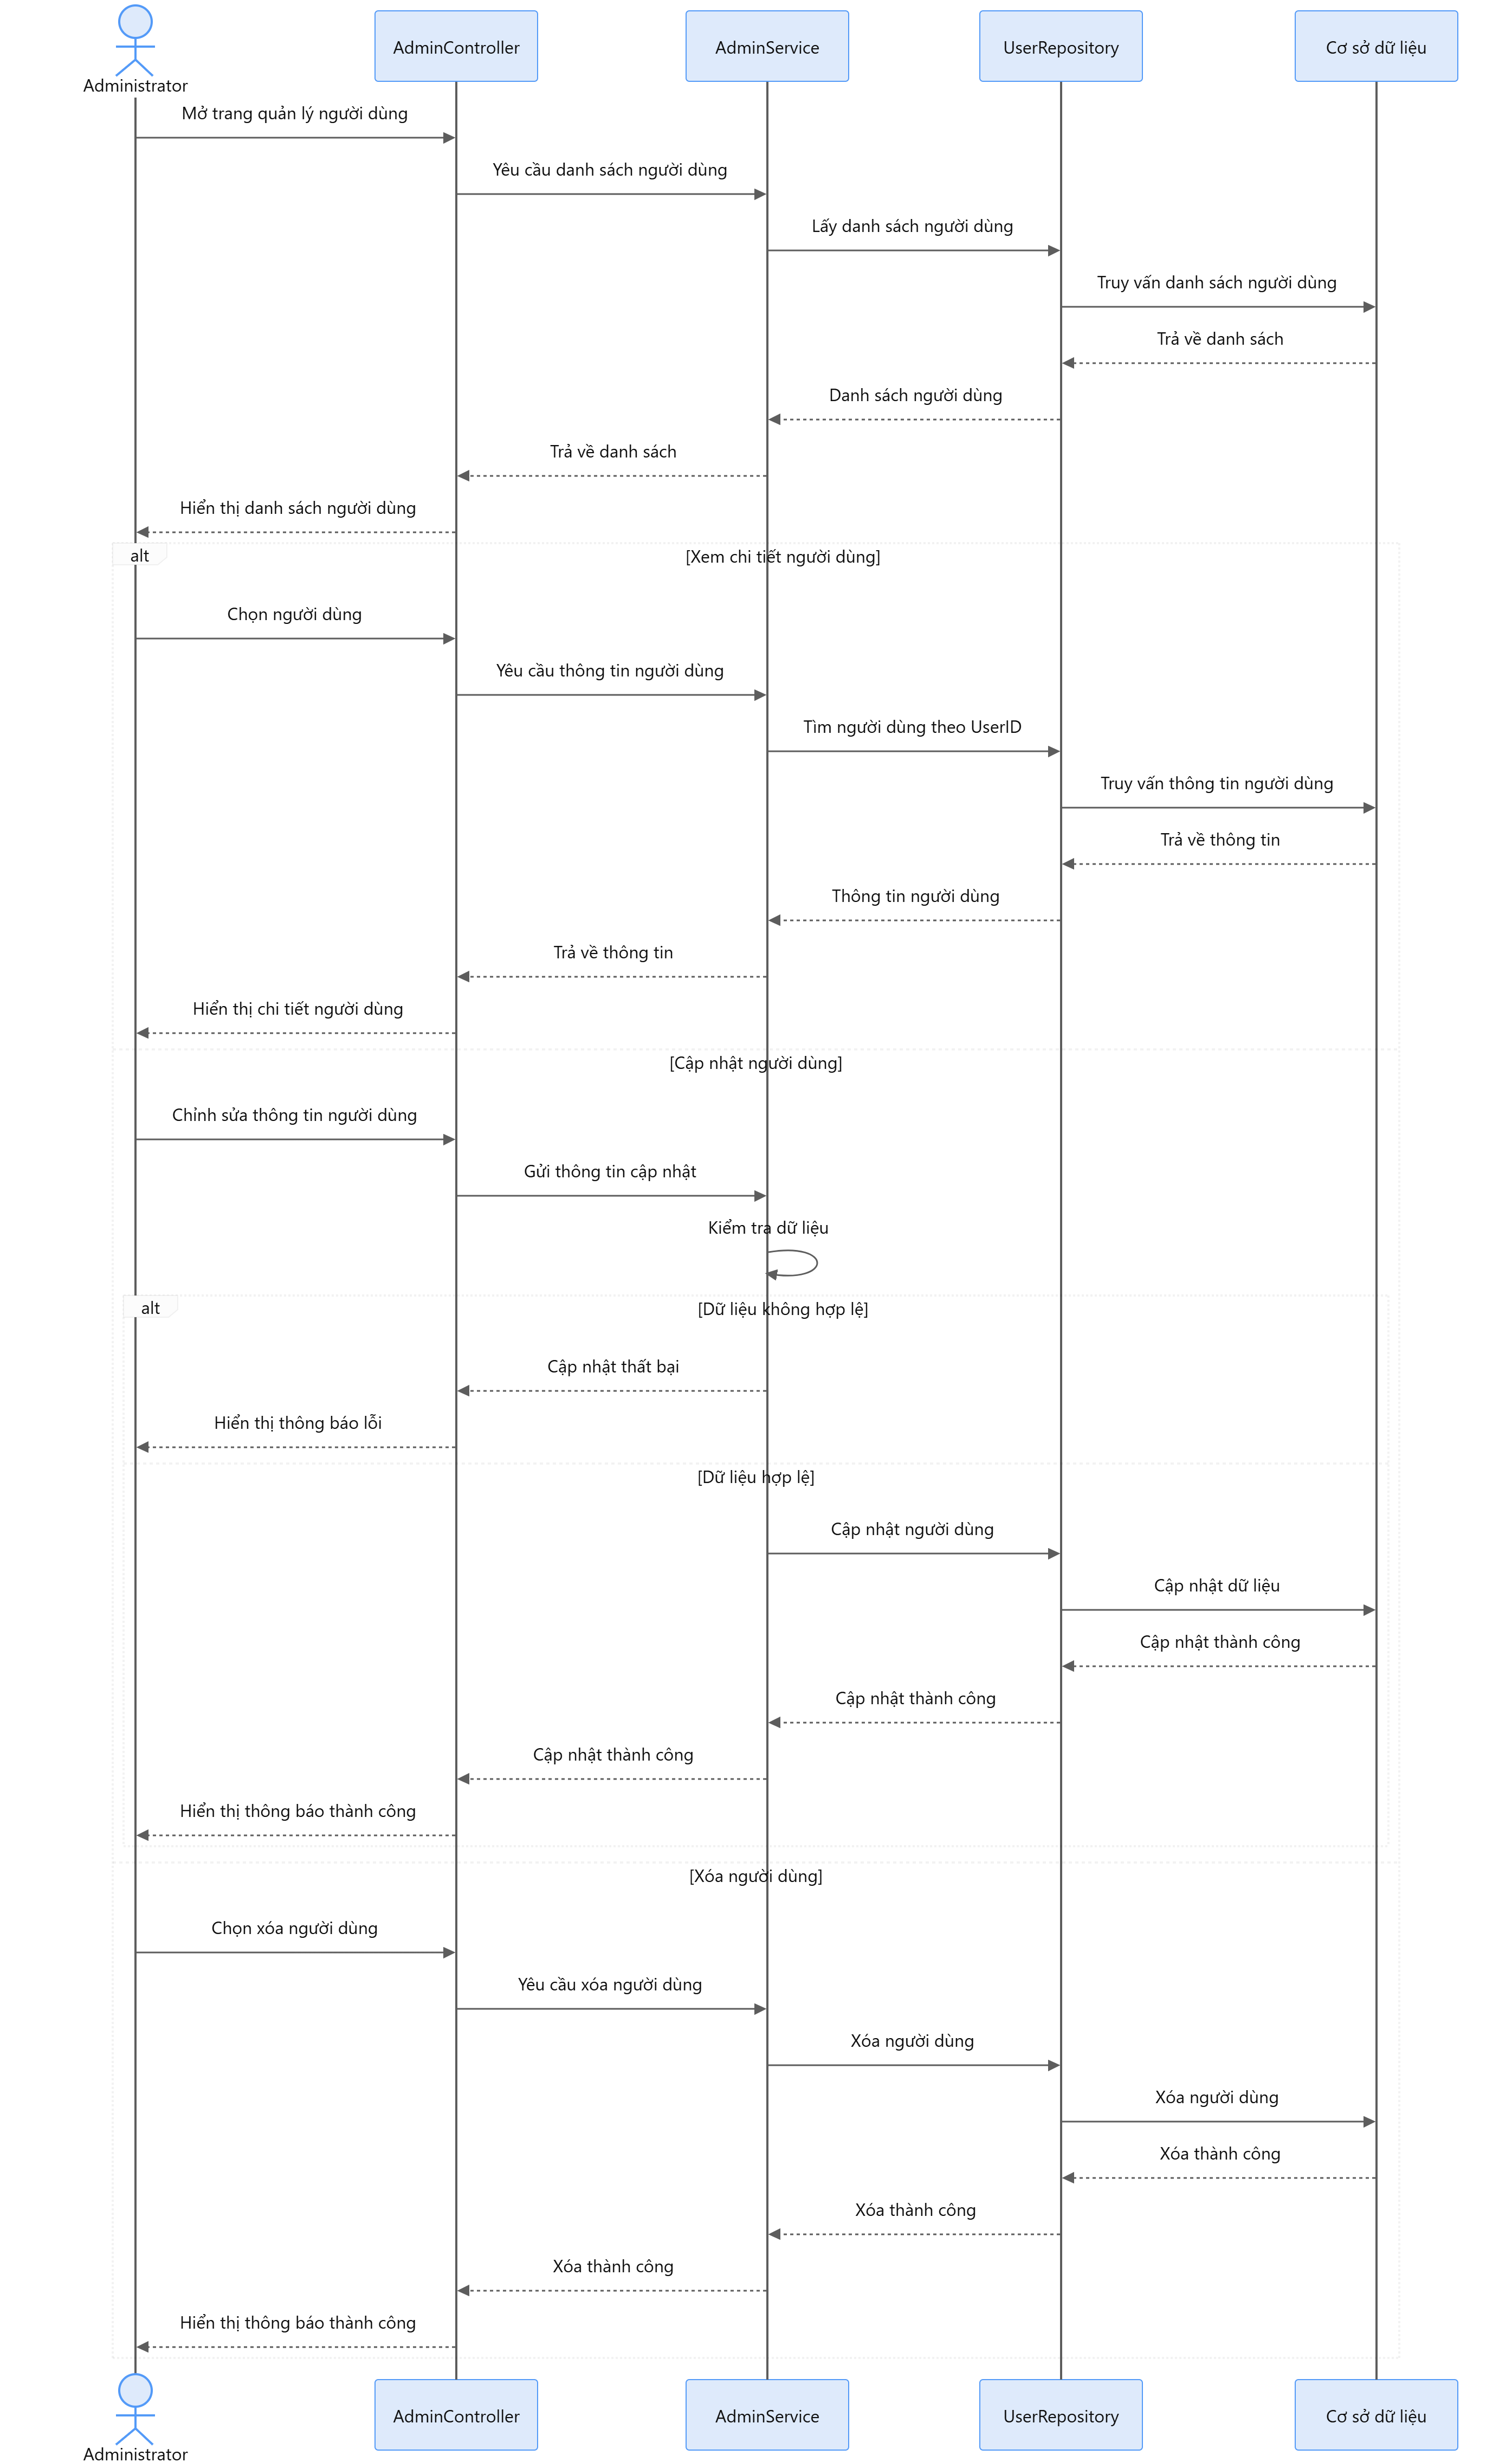
\includegraphics[width=1.1\textwidth]{images/49.png}
\end{figure}


\subsubsection{Quản lý Service Provider}

\paragraph{Class Diagram}

\begin{figure}[H]
	\centering
	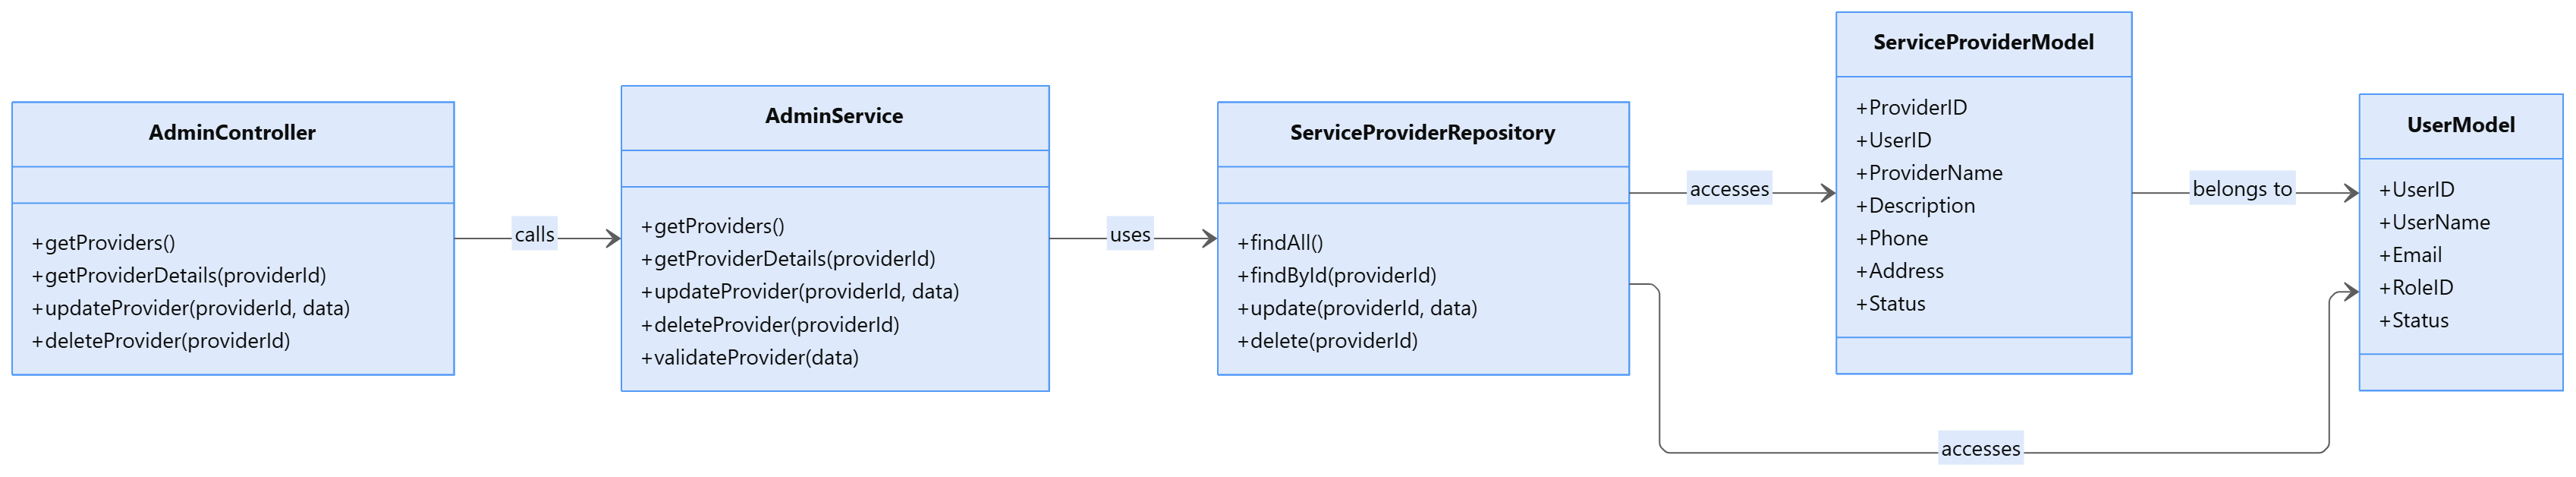
\includegraphics[width=1.1\textwidth]{images/50.png}
\end{figure}

\paragraph{Sequence Diagram}

\begin{figure}[H]
	\centering
	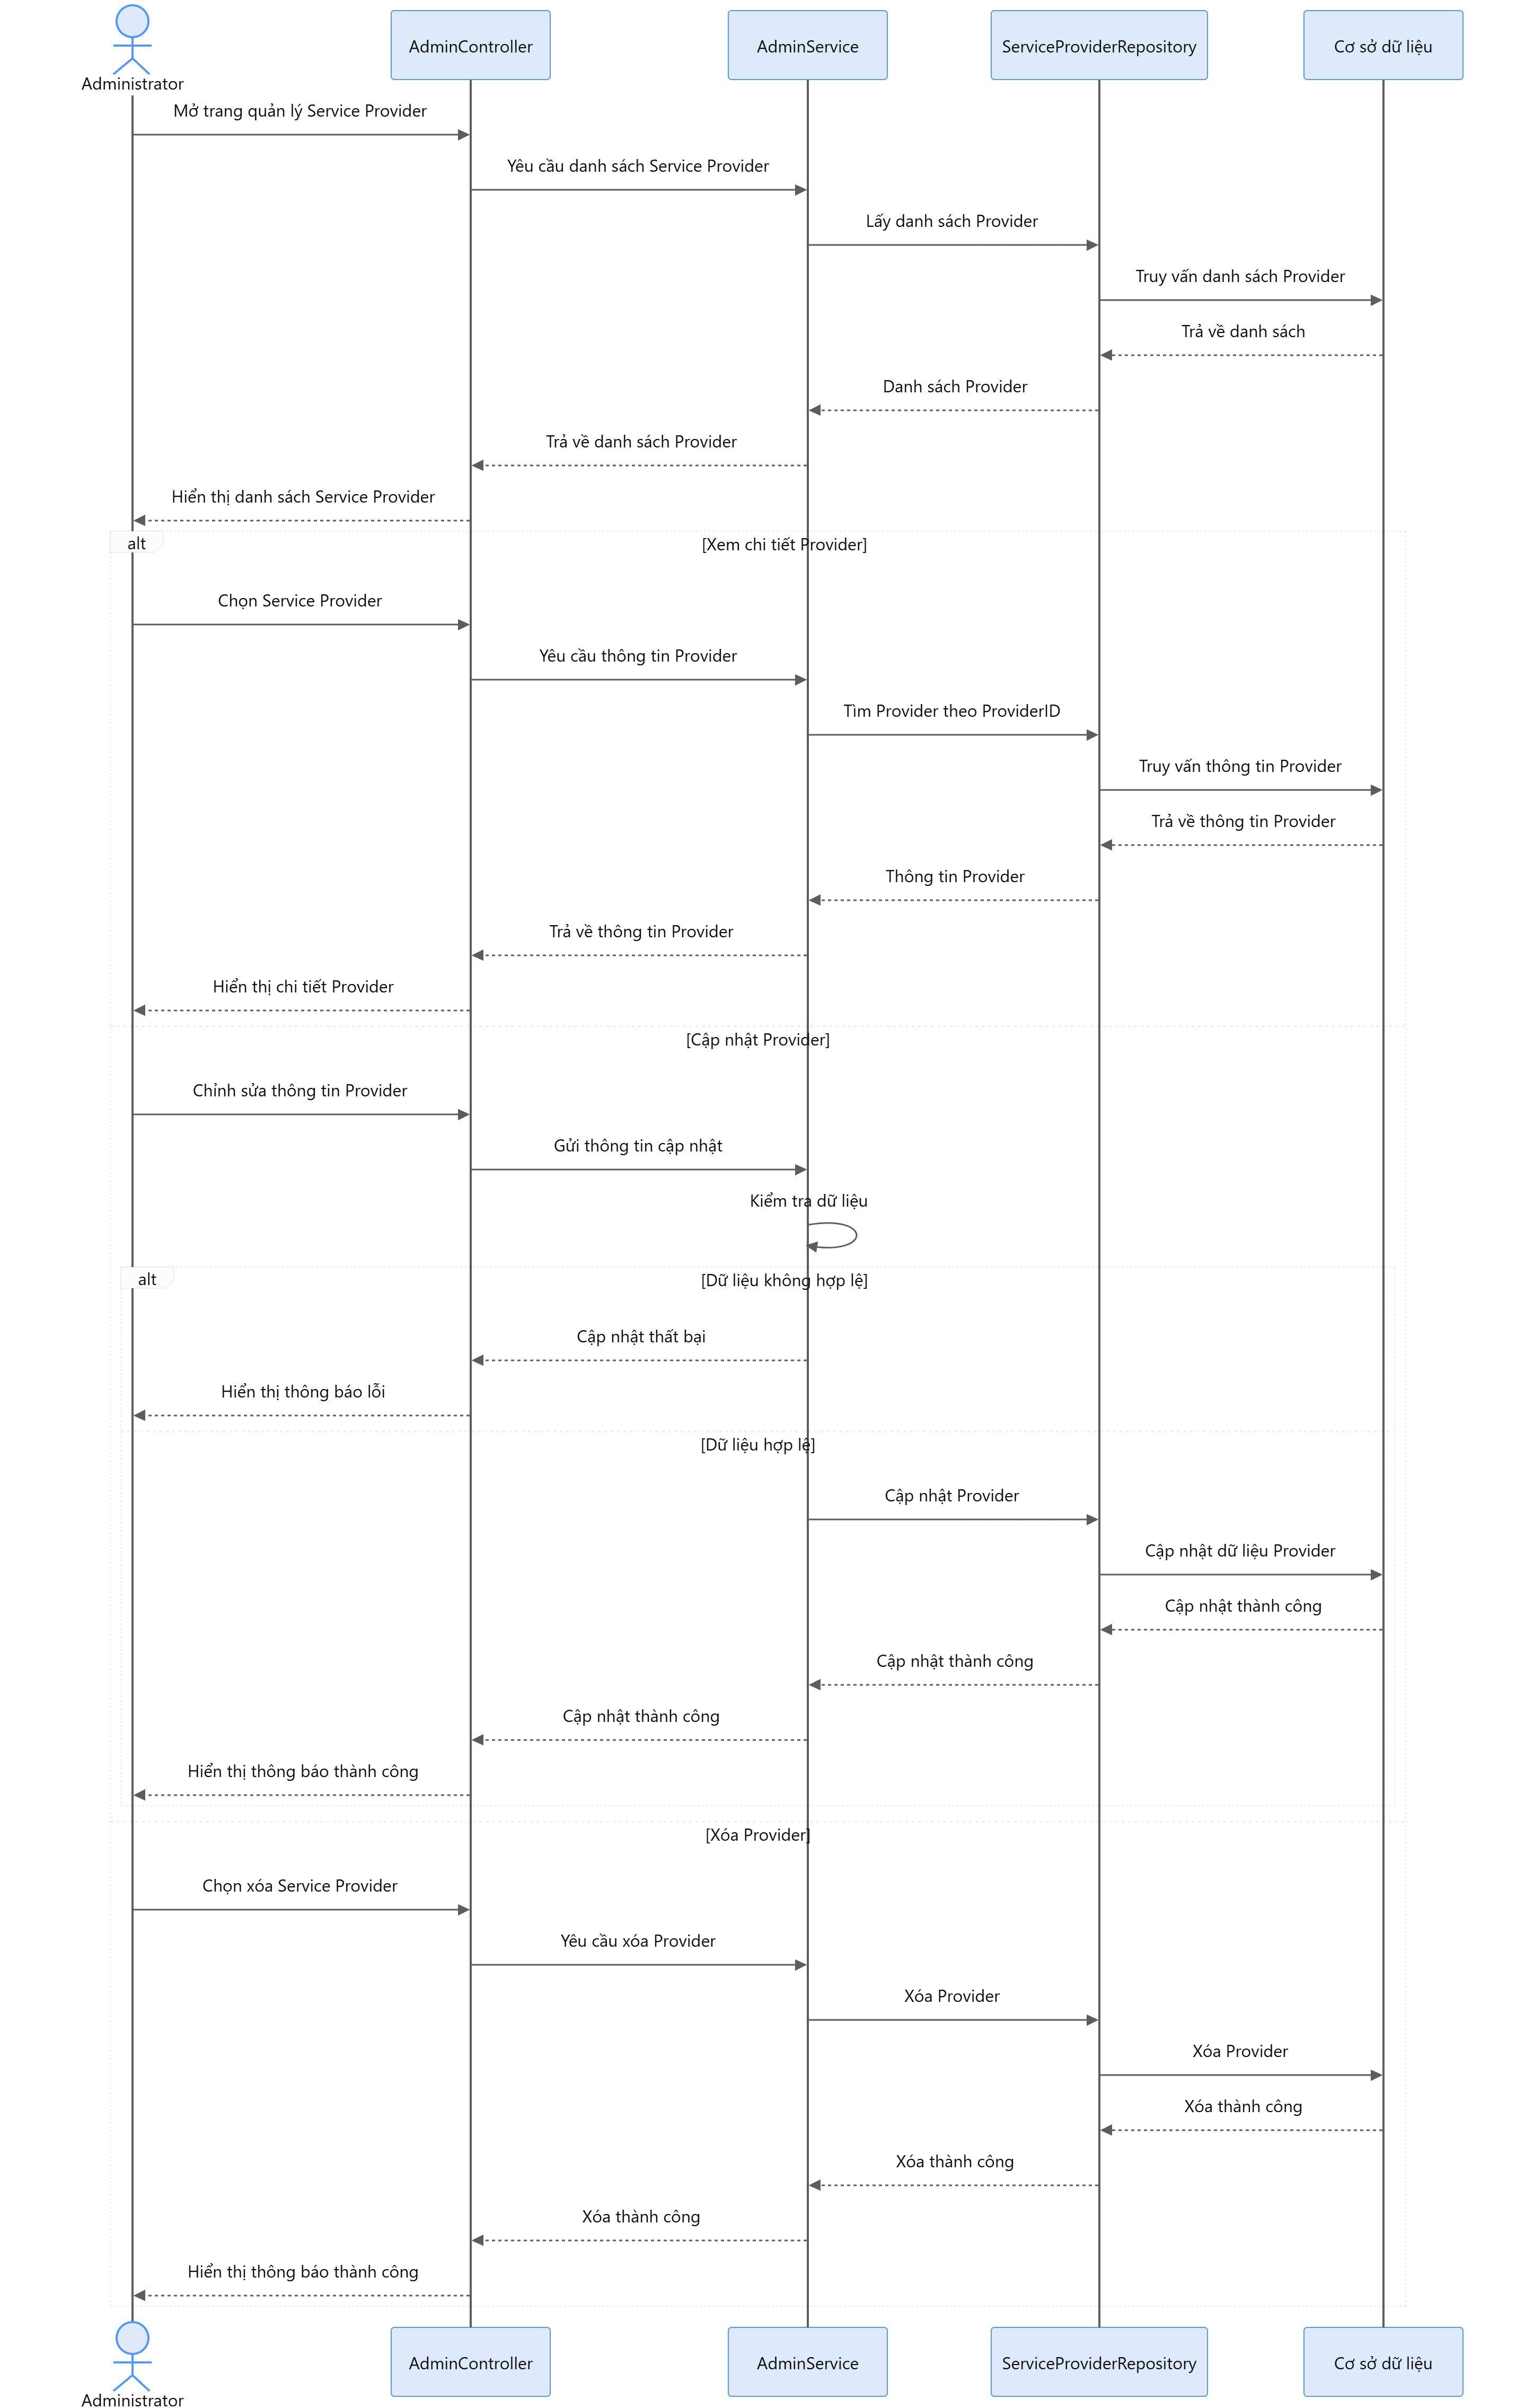
\includegraphics[width=1.1\textwidth]{images/51.png}
\end{figure}


\subsubsection{Phê duyệt Service Provider}

\paragraph{Class Diagram}

\begin{figure}[H]
	\centering
	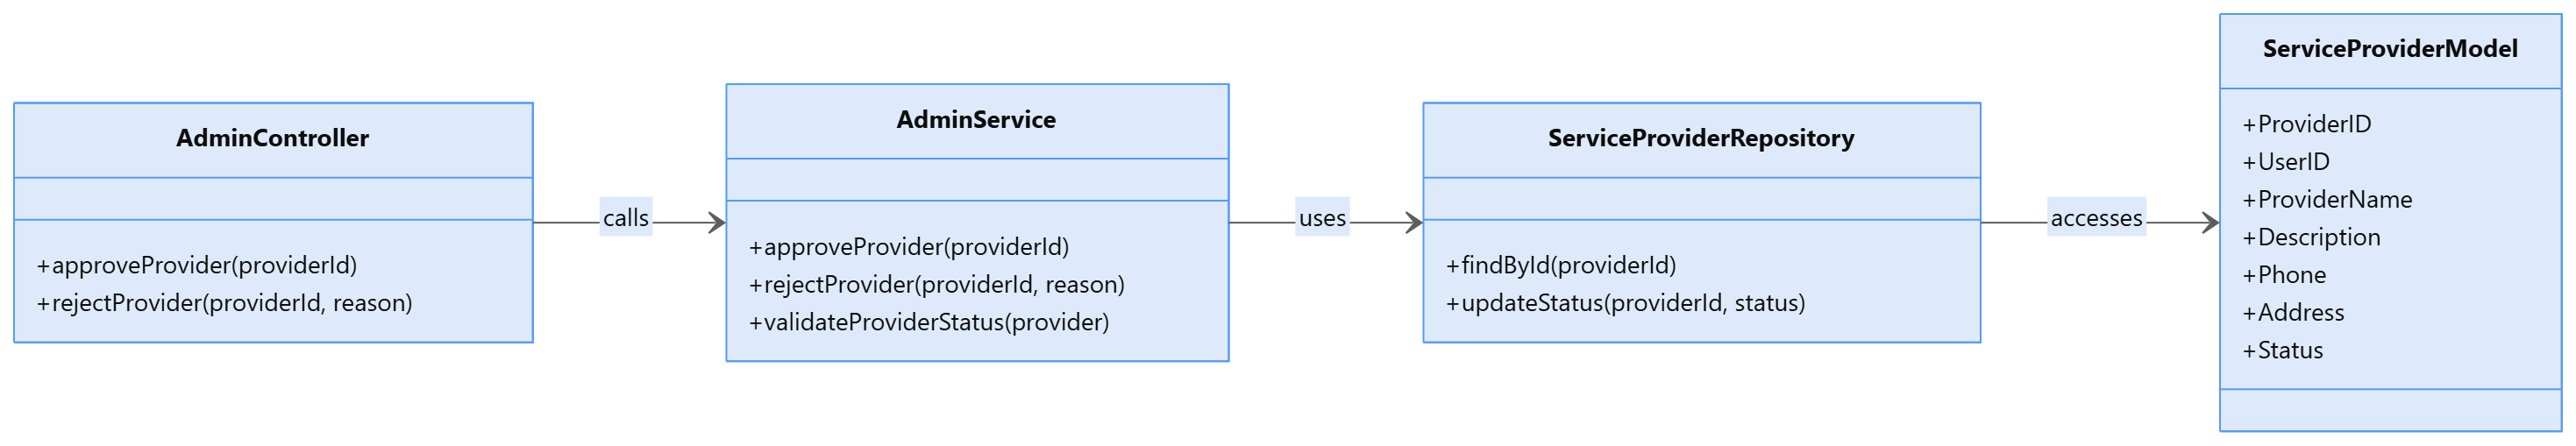
\includegraphics[width=1.1\textwidth]{images/52.png}
\end{figure}

\paragraph{Sequence Diagram}

\begin{figure}[H]
	\centering
	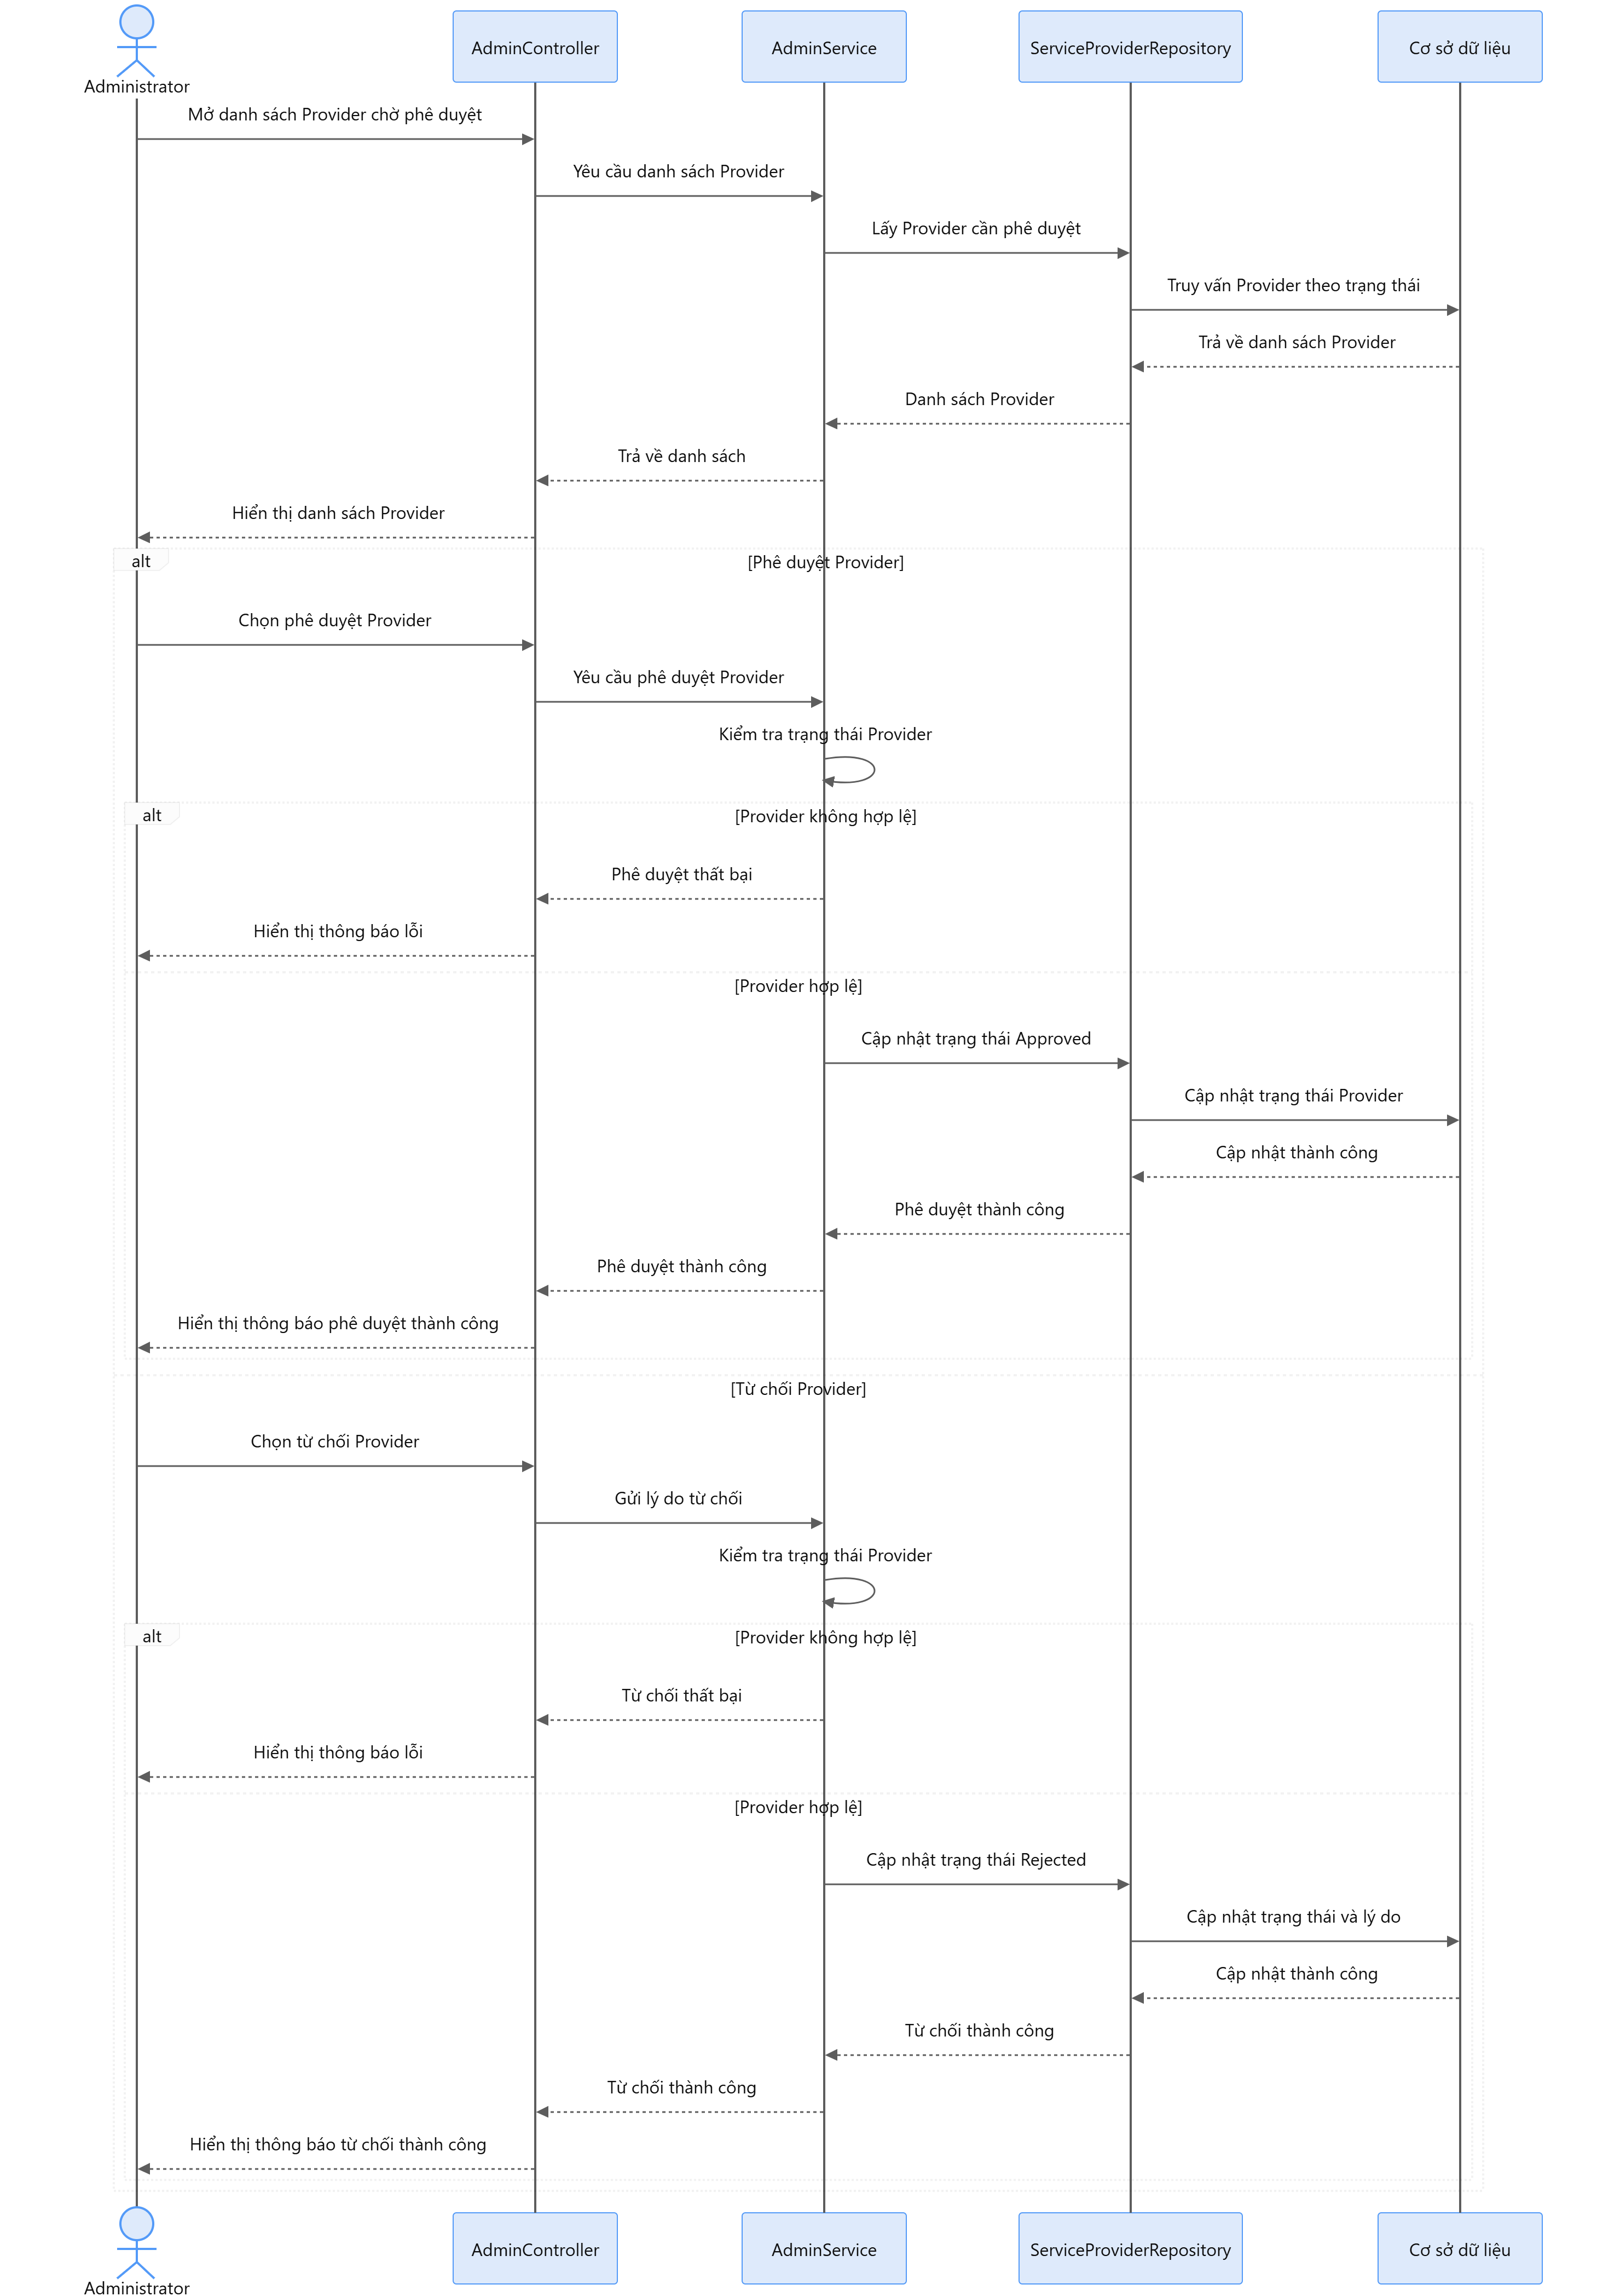
\includegraphics[width=1.1\textwidth]{images/53.png}
\end{figure}
